\documentclass[12pt, a4paper]{article}


% --- PACKAGES --- %
\usepackage[utf8]{inputenc}
\usepackage[T1]{fontenc}
\usepackage[french]{babel}
\usepackage{csquotes}
\usepackage[toc, page]{appendix}
\usepackage{graphicx}
\usepackage{subcaption}
\usepackage{xcolor}
\usepackage{amsmath, amssymb}
\usepackage{amsthm}
\usepackage{mathrsfs}
\usepackage{booktabs}
\usepackage{float}
\usepackage{setspace}
\usepackage{hyperref}
\usepackage{parskip}
\usepackage{caption}
\usepackage{enumitem}
\usepackage{tikz}
\usepackage{tikz-3dplot}
\usepackage{tkz-tab}
\usepackage{dsfont}

% --- BIBLIOGRAPHIE --- %
\usepackage[backend=biber, style=numeric]{biblatex}
\addbibresource{mise_en_page/bibliographie/ter.bib}

% --- MISE EN PAGES --- %
\usepackage{geometry}
\geometry{hmargin=2.5cm,vmargin=2.5cm}
% itemize avec des points
\setlist[itemize,1]{label={\color{black}\small \textbullet}} 
% permet de numéroter les équations en fonction de la section
\numberwithin{equation}{section}
% pour supprimer l'alinéa
\onehalfspacing

% --- QUELQUES COMMANDES --- %
% Ensembles R et N
\newcommand{\bbR}{\mathbb{R}}
\newcommand{\bbN}{\mathbb{N}}
\newcommand{\bbZ}{\mathbb{Z}}

% Lettres
\newcommand{\calF}{\mathcal{F}}
\newcommand{\calK}{\mathcal{K}}
\newcommand{\calD}{\mathcal{D}}
\newcommand{\calR}{\mathcal{R}}
\newcommand{\calL}{\mathcal{L}}
\newcommand{\calM}{\mathcal{M}}
\newcommand{\calB}{\mathcal{B}}
\newcommand{\calE}{\mathcal{E}}

\newcommand{\scrC}{\mathscr{C}}
\newcommand{\scrS}{\mathscr{S}}
\newcommand{\scrA}{\mathscr{A}}

% Commandes maths
% fonctions vectorielles en gras
\usepackage{bm}
\newcommand{\bfm}[1]{\bm{\mathrm{#1}}}
% divergence
\newcommand{\Div}{\mathrm{div}}
% produit scalaire
\newcommand{\ps}[2]{\langle #1, #2 \rangle}
% norme
\newcommand{\norm}[1]{\left\lVert #1 \right\rVert}
% Commande norme triple
\newcommand{\vertiii}[1]{{\left\vert\kern-0.25ex\left\vert
    \kern-0.25ex\left\vert #1 
\right\vert\kern-0.25ex\right\vert\kern-0.25ex\right\vert}}
% valeur absolue
\newcommand{\abs}[1]{\displaystyle\left\lvert #1 \right\rvert}
% exponentielle
\newcommand{\ex}{\mathrm{e}}
% H^1_0(Omega)
\newcommand{\Hone}[1][\Omega]{H^1_0(#1)}
% D(Omega)
\newcommand{\scrD}{\mathscr{D}(\Omega)}
% opérateurs
\newcommand{\operateurs}{M^{-1}_0 L_0}
% limite
\newcommand{\limm}{\underset{h \rightarrow0}{\lim} \ \dfrac{1}{h}}
% ensemble des fonctions à croissances au plus polynomiales
\newcommand{\scrCinfp}{\scrC^{\infty}_p}

% --- NUMEROTATION THEOREMES --- % 
\newtheorem{theoreme}{Théorème}[section]
\newtheorem{proposition}{Proposition}[section]
\newtheorem{definition}{Définition}[section]
\newtheorem{remark}{Remarque}[section]


\begin{document}

% --- PAGE DE GARDE --- %
% =================================================================================
% PAGE DE GARDE PERSONNALISÉE
% =================================================================================
\begin{titlepage}
    \centering
    % --- LOGOS ---
    % Ajustez la largeur (width) si les logos sont trop gros ou trop petits
    \begin{figure}[h]
        \centering
        % Si vous n'avez qu'un seul fichier image avec les deux logos, mettez juste une ligne.
        % Sinon, voici comment mettre deux logos côte à côte :
        
\includegraphics[width=3.5cm]{images/logo_um.png} 
        \hfill 
        
\includegraphics[width=5.5cm]{images/logo_dpt_maths.png}
    \end{figure}
    
    \vspace{1cm}
    
    % --- INFO UNIVERSITÉ ET MASTER ---
    {\Large \textsc{Université de Montpellier}} \\
    \vspace{0.2cm}
    {\large Faculté des Sciences} \\
    \vspace{0.5cm}
    
    \textbf{Master 1 Mathématiques} \\
    % (Monnaie, Banque, Finance, Assurances) \\
    \vspace{0.2cm}
    \textit{Parcours MANU (Modélisation et Analyse Numérique)}
    
    \vspace{2.5cm}
    
    % --- TITRE DU PROJET ---
    \rule{\linewidth}{0.5mm} \\ [0.4cm]
    % { \huge \bfseries Mobilité internationale du capital à l’épreuve des crises récentes : \\ [0.3cm] une réévaluation du puzzle de Feldstein-Horioka } \\ [0.4cm]
    { \huge \bfseries Autour de l'équation de \\[0.3cm] Rayleigh-Stokes} \\ [0.4cm]
    \rule{\linewidth}{0.5mm}
    
    \vspace{2.5cm}
    
    % --- AUTEURS ET RESPONSABLE ---
    \begin{minipage}{0.45\textwidth}
        \begin{flushleft} \large
            \emph{Binôme :}\\
            Hugo \textsc{Johnson}\\
            Quentin \textsc{Lahaye}
        \end{flushleft}
    \end{minipage}
    \begin{minipage}{0.45\textwidth}
        \begin{flushright} \large
            \emph{Responsable :}\\
            Dr. Fabien \textsc{Marche}
        \end{flushright}
    \end{minipage}
    
    \vfill
    
    % --- DATE ET ANNÉE SCOLAIRE ---
    {\large Travail encadré de recherche}\\
    \vspace{0.2cm}
    {\large 29 Mai 2026}\\
    \vspace{0.2cm}
    {\large Année universitaire 2025-2026}
    
\end{titlepage}
\newpage


% --- SOMMAIRE --- %
\tableofcontents
\newpage


% --- INTRODUCTION --- %
% ==================================================================================
% Introduction 
% ==================================================================================

\thispagestyle{empty}
\vspace*{1cm}

\begin{center}
    \Large\textbf{Introduction}
\end{center}

L'équation de Rayleigh-Stokes est une équation aux dérivées partielles utilisée en dynamique des fluides pour modéliser le comportement des fluides non-newtoniens, en particulier les fluides de second grade \footnote{Un \textit{fluide de second grade} ou \textit{fluide de grade $2$} est un modèle de fluide non-newtonien, c'est-à-dire que le tenseur des contraintes n'est plus proportionnel au tenseur des déformations.}. Une forme canonique de l'équation pour une fonction de vitesse $u$ est
\begin{equation*}
    \partial_t u - \nu \Delta u - \alpha \Delta \big(\partial_t u\big) = f
\end{equation*}
où
\begin{itemize}
    \item $\nu$ est la viscosité cinématique du fluide, responsable de la diffusion classique,
    \item $\alpha$ est le paramètre de Rayleigh-Stokes, lié aux propriétés viscoélastiques du fluide,
    \item $f$ est un terme de forçage,
    \item $\Delta \big(\partial_t u\big)$ est un terme dit de \og dispersion régularisée \fg{} qui caractérise le comportement du fluide sous l'effet d'une accélération.
\end{itemize}
Ce modèle trouve des applications dans plusieurs domaines scientifiques. En rhéologie des polymères, il permet de simuler le comportement de fluides qui ne s'écoulent pas instantanément sous l'effet d'un cisaillement. En géophysique, il est utilisé pour modéliser certains mouvements de fluides dans des milieux poreux où les effets de mémoire ne peuvent être négligés. En micro-fluidique, à petite échelle, les forces de surface et les temps de réponse moléculaires deviennent prépondérants, rendant ce type de modèle indispensable. On peut également mentionner le problème de Rayleigh ou premier problème de Stokes, qui décrit l'écoulement engendré par une plaque plane mise soudainement en mouvement dans un fluide visqueux.
\\
C'est d'ailleurs le premier problème de Stokes qui est à l'origine du modèle, car ce n'est pas la forme initiale sous laquelle cette équation est apparue dans la littérature. Nous allons donc revenir aux origines du modèle en nous intéressant au premier problème de Stokes et généraliser le problème en dimension supérieure. Puis, nous allons voir différentes manières d'étudier le problème : dans un premier temps, par une analyse de Fourier en cherchant une solution dans l'espace des distributions tempérées, puis dans les espaces de Sobolev appropriés. Dans cette même section, nous comparerons nos résultats avec l'équation de la chaleur qui est liée à cette équation de Rayleigh-Stokes puisqu'on la retrouve en prenant $\alpha =0$ ; puis dans un second temps, nous allons étudier cette équation par une approche variationnelle sur un domaine borné de $\bbR^d$ avec des conditions de Dirichlet homogènes. Ensuite, nous verrons une première approche numérique avec plusieurs schémas différences finies qui nous permettrons de mettre en évidence la très bonne stabilité numérique de ce problème due au terme $\alpha$. Comme pour l'analyse de Fourier, nous comparerons ces résultats avec ceux sur l'équation de la chaleur. Nous simulerons également quelques cas tests ayant une interprétation physique liée aux applications énoncées précédemment. Enfin, nous terminerons par une approche via la méthode Galerkin discontinu. Nous définirons différents schémas en fonction des bases choisies et nous comparerons nos résultats avec ceux obtenus dans la section précédente sur les schémas différences finies. Nous implémenterons également quelques cas tests similaires aux précédents.
%\newpage


% --- OBJECTIFS --- %
% ==================================================================================
% Objectifs
% ==================================================================================

\thispagestyle{empty}
\vspace*{1cm}

\begin{center}
    \Large\textbf{Nos objectifs}
\end{center}

Voici une présentation succincte de nos objectifs pour ce travail encadré de recherche.

\begin{enumerate}
    \item Bibliographie sur le premier problème de Stokes \cite{Christov2010} dans le but de comprendre le modèle et sa dérivation. Relier cela avec le cours de Mécanique.
    \item Mettre en application les outils vus en Analyse des EDP2 pour réaliser une analyse de Fourier de l'équation.
    \item Comparer les résultats obtenus par analyse de Fourier avec ceux de l'équation de la chaleur, également étudiée en Analyse des EDP2.
    \item Bibliographie sur l'approche variationnelle menée par Showalter et Ting \cite{Showalter_Ting}.
    \item Reproduire l'approche variationnelle de Showalter et Ting. Relier cela avec le cours Analyse numérique 3.
    \item Mettre en application les outils vus en Analyse numérique 1 \& 2 pour définir et étudier un schéma différences finis.
    \item Implémenter en C++ et Python les différents cas tests permettant de mettre en évidence les propriétés du schéma et du paramètre $\alpha$ de l'équation.
    \item Comparer ces résultats avec l'équation de la chaleur qui a été étudiée numériquement en Analyse numérique 1 \& 2.
    \item Implémenter en C++ et Python des cas tests avec un contexte physique.
    \item Proposer un autre schéma différences finis permettant de monter en ordre.
    \item Définir une méthode Galerkin discontinu et l'implémenter en C++ et Python.
\end{enumerate}
\newpage


% --- CORPS DU TEXTE --- %
% ===== Le modèle et sa dérivation ===== %
% =================================================================================
\section{Le modèle}
% =================================================================================

\subsection{Le premier problème de Stokes}
On se place dans un repère orthonormé $(e_1,e_2,e_3)$ et on notera $(x,y,z)$ les composantes d'un point $X$ dans cette base. \`A l'instant initial $t=0$, on considère une plaque immobile d'équation $y=0$ et infinie dans les directions $e_1$ et $e_3$. Dans le demi-espace $y>0$ delimité par cette plaque, on considère un fluide visqueux au repos que l'on suppose incompressible, homogène et ne subissant aucune force extérieure. La plaque est ensuite mise instantanément en mouvement à vitesse constante dans la direction $e_1$. Le problème de Stokes consiste à étudier la vitesse du fluide dans cette situation. 
\\
\begin{figure}[!h]
    \centering
    \tdplotsetmaincoords{70}{120}
    \begin{tikzpicture}[tdplot_main_coords, scale=1.4]
        % ----- PLAQUE (plan y=0, dans le plan xz) -----
        \fill[blue!15, opacity=0.7] (-2.5,-2.5,0) -- (2.5,-2.5,0) -- (2.5,2.5,0) -- (-2.5,2.5,0) -- cycle;
        \draw[gray!60] (-2.5,-2.5,0) -- (2.5,-2.5,0) -- (2.5,2.5,0) -- (-2.5,2.5,0) -- cycle;
        % Label plaque
        \node[blue!60!black] at (2.8, 1.5, 0) {plaque $y=0$};

        % ----- REPÈRE -----
        % Axe x (e1)
        \draw[->, thick] (0,0,0) -- (2.5,0,0) node[anchor=north] {$x$};
        \draw[->, red] (0,0,0) -- (1,0,0) node[above left] {$e_1$};
        % Axe y (e2) vers le haut
        \draw[->, thick] (0,0,0) -- (0,0,2.5) node[anchor=south] {$y$};
        \draw[->, green] (0,0,0) -- (0,0,1) node[right] {$e_2$};
        % Axe z (e3)
        \draw[->, thick] (0,0,0) -- (0,2.5,0) node[anchor=west] {$z$};
        \draw[->, blue] (0,0,0) -- (0,1,0) node[below right] {$e_3$};
        % Origine
        \filldraw[black] (0,0,0) circle (1.5pt) node[below] {$O$};

        % ----- FLUIDE (demi-espace y>0) -----
        \fill[cyan!10, opacity=0.3]
            (-2.5,-2.5,0) -- (2.5,-2.5,0) -- (2.5,-2.5,2.2)
            -- (-2.5,-2.5,2.2) -- cycle;
        \fill[cyan!10, opacity=0.3]
            (2.5,-2.5,0) -- (2.5,2.5,0) -- (2.5,2.5,2.2)
            -- (2.5,-2.5,2.2) -- cycle;
        \fill[cyan!10, opacity=0.3]
            (-2.5,-2.5,2.2) -- (2.5,-2.5,2.2) -- (2.5,2.5,2.2)
            -- (-2.5,2.5,2.2) -- cycle;
        \fill[cyan!10, opacity=0.3]
            (2.5,2.5,0) -- (-2.5,2.5,0) -- (-2.5,2.5,2.2)
            -- (2.5,2.5,2.2) -- cycle;
        \node[cyan!50!black] at (2.2, -1.5, 1.8) {fluide $y>0$};

        % ----- FLÈCHE DE DÉPLACEMENT DE LA PLAQUE -----
        \draw[->, line width=2pt, red!80!black]
            (-0.5, -1.8, 0) -- (1.2, -1.8, 0)
            node[midway, above, sloped] {\small $V e_1$};

        % ----- POINT X -----
        \filldraw[black] (-0.4, 1.0, 1.2) circle (1.5pt);
        \node[above right] at (-0.4, 1.0, 1.2) {$X = (x,y,z)$};
    \end{tikzpicture}
    \caption{Configuration du premier problème de Stokes}
    \label{fig:pbmStokes}
\end{figure}
\\
On considère donc la vitesse du fluide
\begin{eqnarray*}
    \bfm{u} : \bbR^3 \times \bbR_+ &\longrightarrow& \bbR^3 \\
    (X,t) &\longmapsto& \big(u_1(X,t), u_2(X,t), u_3(X,t)\big)
\end{eqnarray*}
Le contexte du premier problème de Stokes nous amène à quelques simplifications. La plaque étant infinie dans les directions $e_1$ et $e_3$, la vitesse du fluide ne dépendra pas de $x$ et $z$, on notera donc plus simplement
\begin{equation*}
    \bfm{u} (X,t) = \bfm{u} (y,t)
\end{equation*}
La plaque étant mise en mouvement uniquement dans la direction $e_1$, on obtient un écoulement unidirectionnel. On pose alors
\begin{equation*}
    \bfm{u} (y,t) = \big(u_1(y,t),0,0\big)
\end{equation*}
De plus, on supposera $\bfm{u}$ suffisamment régulière afin de simplifier les calculs. On utilise d'abord l'équation de conservation de la masse
\begin{equation}\label{consevermationmasse1}
    \frac{D\rho}{Dt} + \rho \Div(\bfm{u}) = 0
\end{equation}
où $\rho(X,t)$ est la densité du fluide et $\dfrac{D}{Dt}$ est la dérivée particulaire définie par
\begin{equation*}
    \frac{D}{Dt} := \partial_t  +  \bfm{u} \cdot \nabla 
\end{equation*}
Comme le fluide est incompressible et homogène $\dfrac{D\rho}{Dt} = 0$, donc 
$\rho$ est une fonction constante que l'on notera dans la suite $\rho >0$ et \eqref{consevermationmasse1} devient $\Div(\bfm{u})=0$. Puis, les équations du mouvement du milieu continu nous donne 
\begin{equation}\label{PFD1}
    \rho \frac{D\bfm{u}}{Dt} = \Div(\sigma) + \rho \bfm{f}
\end{equation}
où $\sigma$ est le tenseur des contraintes et le terme $\rho\bfm{f}$ représente les forces massiques de densité volumique. Les hypothèses du problème de Stokes nous donnent la simplification $\bfm{f}=0$ et 
\begin{equation*}
    \frac{D\bfm{u}}{Dt} = \partial_t \bfm{u} + (\bfm{u} \cdot \nabla) \bfm{u} = \partial_t u_1 + \begin{pmatrix}
        0 & \partial_yu_1 & 0 \\
        0 & 0 & 0 \\
        0 & 0 & 0
    \end{pmatrix}\begin{pmatrix}
        u_1 \\ 0 \\ 0
    \end{pmatrix} = \partial_tu_1
\end{equation*}
C'est l'équation \eqref{PFD1} qui va nous donner l'équation de Rayleigh-Stokes, il nous faut donc déterminer $\sigma$. Pour un fluide de second grade, le tenseur des contraintes est donné par le théorème de Rivlin-Ericksen 
\begin{equation*}
    \sigma := -pI + \mu A_1 + \alpha_1 A_2 + \alpha_2 A_1^2
\end{equation*}
où
\begin{itemize}
    \item $pI$ est la contrainte isotropique avec $p$ la pression,
    \item $A_1 := \nabla \bfm{u} + \nabla^t \bfm{u}$,
    \item $A_2 := \dfrac{D}{Dt}A_1 + A_1\nabla \bfm{u} + \nabla^t\bfm{u} A_1$,
    \item $\mu >0$ est la viscosité du fluide,
    \item $\alpha_1$ et $\alpha_2$ sont des paramètres thermodynamiques qui doivent vérifier 
    \begin{eqnarray*}
        \alpha_1 \geq 0 \ \ \ \ \ \text{ et } \ \ \ \ \ \alpha_1 + \alpha_2 = 0
    \end{eqnarray*}
    pour que le modèle soit physiquement admissible.
\end{itemize}

\begin{remark}
    Concernant le \og théorème de Rivlin-Ericksen \fg{} cité, nous faisons allusions ici à l'article \cite{Rivlin1955} dans lequel  Rivlin et Ericksen établissent, pour un fluide de grade $n$, le lien (section $37$) entre le tenseur des contraintes $\sigma$ et les tenseurs dit de Rivlin-Ericksen $A_1, A_2, \dots, A_n$, qui sont définis par récurrence par 
    \begin{eqnarray*}
        A_1 &=& \nabla \bfm{u} + \nabla^t \bfm{u} \\
        \forall k \in \bbN, \ A_{k+1} &=& \frac{D}{Dt}A_k + A_k \nabla \bfm{u} + \nabla^t\bfm{u}A_k
    \end{eqnarray*}
    Le tenseur des contraintes $\sigma$ est une fonction tensorielle isotrope de $A_1,\dots, A_n$, c'est-à-dire que
    \begin{equation*}
        \sigma(A_1,\dots,A_n) = \varphi_0 I + \varphi_1 A_1 + \varphi_2A_2 + \varphi_3A_1^2 + \cdots
    \end{equation*}
    où les $\varphi_i$ sont des fonctions scalaires, et que pour tout $Q \in O_3(\bbR)$ on a 
    \begin{equation*}
        \sigma(QA_1Q^t, \dots, QA_nQ^t) = Q \sigma (A_1,\dots, A_n) Q^t
    \end{equation*}
    Autrement dit, si on fait une subir une rotation au fluide, le tenseur des contraintes subi aussi cette rotation. Donc, dans notre cas
    \begin{equation*}
        \sigma(A_1,A_2) = \varphi_0 I + \varphi_1 A_1 + \varphi_2A_2 + \varphi_3A_1^2
    \end{equation*}
    Puis, dans la section $38$, ils donnent les formes explicites des coefficients $\varphi_i$, ce sont des fonctions des invariants scalaires des tenseurs $A_1,\dots, A_n$. Dans notre cas, ils peuvent être associés à des paramètres physiques liés au fluide étudié : $\mu$, $\alpha_1$ et $\alpha_2$. \\
\end{remark}

\begin{remark}
    Si on suppose $\alpha_1<0$, il est possible de montrer qu'un écoulement comme le cisaillement simple entre deux plaques parallèles est instable, et même que pour certaines distances entre les deux plaques, l'écoulement n'existe pas. Pour plus de détails sur les rôles de $\alpha_1$ et $\alpha_2$ nous renvoyons à la référence \cite[p.~211]{thermo_fluid_2}.
\end{remark}

On obtient 
\begin{eqnarray*}
    A_1 = \begin{pmatrix}
        0 & \partial_yu_1 & 0 \\
        \partial_yu_1 & 0 & 0 \\
        0 & 0 & 0
    \end{pmatrix} \ \ \ &\text{ et }& \ \ \ A_1^2 = \begin{pmatrix}
        (\partial_yu_1)^2 & 0 & 0 \\
        0 & (\partial_y u_1)^2 & 0 \\
        0 & 0 & 0
    \end{pmatrix}
\end{eqnarray*}
En écrivant, $\dfrac{D}{Dt}A_1$ dans la définition de $A_2$, on entend appliquer l'opérateur $\dfrac{D}{Dt}$ à chaque composante de $A_1$, d'où
\begin{eqnarray*}
    A_2 &=& \dfrac{D}{Dt}A_1 + A_1\nabla \bfm{u} + \nabla^t\bfm{u} A_1 \\
    &=& \begin{pmatrix}
        0 & \partial_{ty} u_1 & 0 \\
        \partial_{ty}u_1 & 0 & 0 \\
        0 & 0 & 0
    \end{pmatrix} + \begin{pmatrix}
        0 & 0 & 0 \\
        0 & (\partial_yu_1)^2 & 0 \\
        0 & 0 & 0
    \end{pmatrix} + \begin{pmatrix}
        0 & 0 & 0 \\
        0 & (\partial_yu_1)^2 & 0 \\
        0 & 0 & 0
    \end{pmatrix} \\
    &=& \begin{pmatrix}
        0 & \partial_{ty}u_1 & 0 \\
        \partial_{ty} u_1 & 2(\partial_yu_1)^2 & 0 \\
        0 & 0 & 0
    \end{pmatrix}
\end{eqnarray*}
Finalement, le tenseur des contraintes est
\begin{equation*}
    \sigma = \begin{pmatrix}
        -p+\alpha_2(\partial_yu_1)^2 & \mu\partial_yu_1 + \alpha_1 \partial_{ty}u_1 & 0 \\
        \mu \partial_yu_1+\alpha_1\partial_{ty} u_1 & -p+(2\alpha_1+\alpha_2)(\partial_yu_1)^2 & 0 \\
        0 & 0 & -p
    \end{pmatrix}
\end{equation*}
On injecte dans \eqref{PFD1} et on obtient
\begin{equation*}
    \left\{\begin{array}{rcl}
        \rho\partial_tu_1 & = & -\partial_xp + \alpha_2\partial_x(\partial_yu_1)^2 + \mu \partial_{yy}u_1 + \alpha_1 \partial_{yty}u_1  \\
        0 & = & \mu \partial_{xy}u_1 + \alpha_1\partial_{xty}u_1 - \partial_yp+(2\alpha_1+\alpha_2)\partial_y(\partial_yu_1)^2 \\
        0 & = & - \partial_zp
    \end{array}\right.
\end{equation*}
on utilise l'indépendance de $u_1$ en $x$ et $z$ pour simplifier le système
\begin{equation*}
    \left\{\begin{array}{rcl}
        \rho\partial_tu_1 & = & -\partial_xp + \mu \partial_{yy}u_1 + \alpha_1 \partial_{yty}u_1  \\
        0 & = & - \partial_yp+2(2\alpha_1+\alpha_2)\partial_yu_1\partial_{yy}u_1 \\
        0 & = & - \partial_zp
    \end{array}\right.
\end{equation*}
L'invariance par translation dans les directions $e_1$ et $e_3$ implique que la pression ne dépend pas de $x$ et $z$, donc $\partial_xp=0$. En réorganisant les termes de la première équation du système, on obtient finalement l'équation de Rayleigh-Stokes homogène en une dimension
\begin{equation*}
    \partial_t u_1 - \nu \partial_{yy}u_1 - \alpha \partial_{tyy}u_1=0
\end{equation*}
où $\nu := \dfrac{\mu}{\rho}$ et $\alpha := \dfrac{\alpha_1}{\rho}$.

\subsection{Dérivation de l'équation de Rayleigh-Stokes scalaire multidimensionnelle}\label{RS_scalaire}
Dans cette section, l'objectif est de généraliser l'équation de Rayleigh-Stokes scalaire en conservant un cadre $3$D spatial. Le cadre physique reste similaire, on considère l'écoulement unidirectionnel (dans la direction $e_1$ comme sur la figure \ref{fig:pbmStokes}) d'un fluide de grade $2$, incompressible et homogène de densité $\rho>0$. On note $\bfm{u} : \bbR^3 \times \bbR_+ \rightarrow \bbR^3$ la vitesse du fluide que l'on supposera suffisamment régulière. Les équations du mouvement du milieu continu nous donne 
\begin{equation}\label{PFD_1}
    \rho \frac{D\bfm{u}}{Dt} = \Div(\sigma) + \rho \bfm{f}
\end{equation}
où $\sigma$ est le tenseur des contraintes et le terme $\rho \bfm{f}$ représente les forces massiques de densité volumique que l'on supposera nulles. Pour un fluide de second grade, le tenseur des contraintes est donné par le théorème de Rivlin-Ericksen 
\begin{equation*}
    \sigma := -pI + \mu A_1 + \alpha_1 A_2 + \alpha_2 A_1^2
\end{equation*}
où on utilise les mêmes notations qu'à la section précédente. On a donc 
\begin{eqnarray*}
    \Div(\sigma) = -\nabla p + \mu \Delta \bfm{u} + \alpha_1\Div(A_2) + \alpha_2\Div(A_1^2)
\end{eqnarray*}
On injecte cette expression dans \eqref{PFD_1} et on obtient les équations de Navier-Stokes pour un fluide incompressible, homogène de grade $2$
\begin{equation}\label{NS_gen}
    \left\{\begin{array}{l}
        \rho\big(\partial_t\bfm{u} + (\bfm{u} \cdot\nabla)\bfm{u}\big) = -\nabla p + \mu \Delta \bfm{u} + \alpha_1 \Div(A_2) + \alpha_2 \Div(A_1^2)  \\
        \Div(\bfm{u}) = 0 
    \end{array}\right.
\end{equation}
L'écoulement étant unidirectionnel dans la direction $e_1$, notre vitesse $\bfm{u}$ est de la forme
\begin{equation*}
    \bfm{u}(X,t) = (u_1(X,t),0,0)
\end{equation*}
On utilise l'incompressibilité qui donne
\begin{eqnarray*}
    \Div(\bfm{u}) = 0 &\Longrightarrow& \partial_xu_1(x,y,z,t) = 0
\end{eqnarray*}
donc $u_1$ ne dépend pas de la variable $x$. Puis on linéarise l'équation vectorielle de \eqref{NS_gen}, ainsi
\begin{eqnarray*}
    A_2 \approx \partial_t A_1 \ \ \ \text{ et } \ \ \ A_1^2 \approx 0
\end{eqnarray*}
donc 
\begin{align*}
    \Div(A_1) &= \nabla(\Div(\bfm{u})) + \Delta \bfm{u} &\text{ et }&& \Div(\partial_tA_1) &=\nabla\big(\partial_t(\Div(\bfm{u}))\big) + \Delta\big(\partial_t \bfm{u}\big)
\end{align*}
ensuite, en utilisant l'incompressibilité, on obtient 
\begin{eqnarray*}
    \Div(A_1) = \Delta \bfm{u} \ \ \ \text{ et } \ \ \ \Div(A_2) = \Delta\big(\partial_t \bfm{u}\big)
\end{eqnarray*}
enfin,
\begin{equation*}
    \Div(pI) = \nabla p
\end{equation*}
finalement,  
\begin{equation*}
    \Div(\sigma) = -\nabla p +\mu \Delta \bfm{u} + \alpha_1 \Delta\big(\partial_t \bfm{u} \big)
\end{equation*}
Alors l'équation vectorielle de \eqref{NS_gen} devient
\begin{eqnarray*}
    \rho \partial_t \bfm{u} = -\nabla p + \mu \Delta \bfm{u} + \alpha_1 \Delta\big(\partial_t\bfm{u}\big)
    &\iff& \left\{\begin{array}{l}
        \rho \partial_t u_1 = \partial_xp + \mu\Delta u_1 + \alpha_1 \Delta \big(\partial_t u_1\big) \\
        0 = -\partial_y p \\
        0 = - \partial_z p
    \end{array}\right.
\end{eqnarray*}
Ce système nous donne $\partial_y p = \partial_z p =0$, donc la pression $p$ dépend uniquement de la variable d'espace $x$. Il nous reste l'équation scalaire
\begin{equation*}
    \rho \partial_t u_1(y,z,t) = \partial_xp(x,t) + \mu\Delta u_1(y,z,t) + \alpha_1 \Delta \big(\partial_t u_1(y,z,t)\big)
\end{equation*}
où $\Delta = \partial_{yy}+\partial_{zz}$. Par séparation des variables, on obtient $\partial_xp$ qui est constant ou bien $\partial_xp$ est une fonction de $t$ uniquement. Ici, on souhaite que le mouvement soit généré uniquement par le déplacement d'une paroi, on postule que le fluide est au repos à l'infini avec une pression uniforme. Dans ce cas, il n'y a aucune force motrice externe pour créer une différence de pression. On pose donc $\partial_xp=0$. C'est cette hypothèse qui caractérise un écoulement de Rayleigh (entraînement par la paroi) plutôt qu'un écoulement de Poiseuille (entraînement par la pression). On obtient l'équation de Rayleigh-Stokes homogène
\begin{equation*}\label{eq_RS_scalaire}
    \partial_t u_1 - \nu \Delta u_1 - \alpha \Delta \big(\partial_t u_1\big)=0
\end{equation*}
où $\nu := \dfrac{\mu}{\rho}$ et $\alpha := \dfrac{\alpha_1}{\rho}$.

\subsection{Dérivation de l'équation de Rayleigh-Stokes vectorielle multidimensionnelle}\label{RS_vectorielle}
Soit $d \in \bbN$ la dimension. On veut maintenant généraliser l'équation scalaire obtenue en une équation vectorielle. On considère toujours un fluide de grade $2$, incompressible et homogène de densité $\rho>0$. On note la vitesse du fluide $\bfm{u}:\bbR^d \times \bbR_+ \rightarrow \bbR^d$ que l'on supposera suffisamment régulière. On va reproduire le raisonnement de la première section, sans les hypothèses du premier problème de Stokes, en linéarisant par rapport à $\nabla \bfm{u}$. Les équations du mouvement du milieu continu nous donnent 
\begin{equation}\label{PFD2}
    \rho \frac{D\bfm{u}}{Dt} = \Div(\sigma) + \rho \bfm{f}
\end{equation}
où $\sigma$ est le tenseur des contraintes et $\bfm{f}$ les forces extérieures. Pour un fluide de second grade, le tenseur des contraintes est donné par le théorème de Rivlin-Ericksen
\begin{equation*}
    \sigma := -pI + \mu A_1 + \alpha_1 A_2 + \alpha_2 A_1^2
\end{equation*}
où on conserve les notations des sections précédentes. Comme dans la section précédente, l'hypothèse de linéarisation nous donne 
\begin{equation*}
    \frac{D\bfm{u}}{Dt} = \partial_t\bfm{u} + (\bfm{u} \cdot \nabla)\bfm{u} \approx \partial_t \bfm{u}
\end{equation*}
et 
\begin{equation*}
    \sigma \approx -pI + \mu A_1 + \alpha_1\partial_tA_1
\end{equation*}
Donc 
\begin{equation*}
    \Div(\sigma) = -\nabla p +\mu \Delta \bfm{u} + \alpha_1 \Delta\big(\partial_t \bfm{u} \big)
\end{equation*}
On remplace dans \eqref{PFD2} et on réorganise les termes, on obtient alors 
\begin{equation*}
    \partial_t\bfm{u} - \frac{\mu}{\rho}\Delta \bfm{u} - \frac{\alpha_1}{\rho}\Delta \big(\partial_t \bfm{u}\big) +\frac{1}{\rho}\nabla p= \bfm{f} 
\end{equation*}
En posant, $\nu := \mu/\rho$, $\alpha := \alpha_1/\rho$, et $\tilde{p}=p/\rho$ on parvient finalement au système d'inconnues $(\bfm{u}, \tilde{p})$
\begin{equation}\label{eq_RS}
    \left\{\begin{array}{l}
         \partial_t\bfm{u} - \nu\Delta \bfm{u} - \alpha\Delta \big(\partial_t \bfm{u}\big) = -\nabla \tilde{p} + \bfm{f}  \\
         \Div (\bfm{u}) = 0
    \end{array}\right.
\end{equation}

\newpage

% ===== Analyse mathématique ===== %
% ----- Approche variationnelle ----- %
% ==========================================================================
\section{Analyse mathématique}
% =========================================================================

\subsection{Analyse de Fourier}

Dans cette section, on considère le problème
\begin{equation*}
    \begin{cases}
        \partial_tu(t,x) - \nu\Delta u(t,x) - \alpha\Delta \big(\partial_t u(t,x)\big) = 0 & (t,x) \in \mathbb R_+ \times \bbR^d  \\
        u(0,x) = u_0(x) & x \in \bbR^d
    \end{cases}
\end{equation*}
où l'on précisera la régularité de la donnée initiale $u_0$ dans les sections suivantes. On prendra pour convention la transformée de Fourier \og normalisée \fg{}
définie par
\begin{equation*}
    \hat{u}(\xi)=\calF\big(u(x)\big)(\xi) = \frac{1}{(2\pi)^{d/2}}\int_{\bbR^d} \ex^{-ix\cdot\xi}u(x)\mathrm{d}x
\end{equation*}
le contexte étant suffisament clair, on notera plus simplement $x\xi$ le produit scalaire $x \cdot \xi$. Soit $s \in \bbR$ l'exposant pour les espaces de Sobolev.
\subsubsection{Donnée initiale dans \texorpdfstring{$\scrS'(\bbR^d)$}{S'(Rd)}}
On considère $u_0 \in \scrS'(\bbR^d)$. Comme dans la section précédente, on peut reformuler le problème précédent de la façon suivante : trouver $u \in \scrC^1(\bbR_+, \scrS'(\bbR^d))$ tel que 
\begin{equation}\label{pb_RS4}
    \begin{cases}
        u'(t) - \nu\Delta u(t) - \alpha\Delta \big(u'(t)\big) = 0  \\
        u(0) = u_0
    \end{cases}
\end{equation}
\paragraph{Unicité.} On suppose qu'il existe une solution $u \in \scrC^1(\bbR_+,\scrS'(\bbR^d))$. On applique la transformée de Fourier au problème \eqref{pb_RS4}. On obtient pour la donnée initiale
\begin{equation*}
    \hat{u}(0) = \hat{u}_0
\end{equation*}
et pour l'équation, on utilise la linéarité de $\calF$
\begin{equation*}
    \calF\big(u'(t)\big)-\nu\calF\big(\Delta u(t)\big)-\alpha\calF\big(\Delta(u'(t))\big) = 0
\end{equation*}
Montrons que $\calF\big(u'(t)\big)=\hat{u}'(t)$. On étudie d'abord la dérivabilité de $t \mapsto \hat{u}(t)$. Soient $t \in \bbR_+$ et $h>0$. On a par linéarité de $\calF$
\begin{equation*}
    \frac{\hat{u}(t+h)-\hat{u}(t)}{h} = \calF\bigg(\frac{u(t+h)-u(t)}{h}\bigg)
\end{equation*}
comme par hypothèse, $u \in \scrC^1(\bbR_+,\scrS'(\bbR^d))$ on a
\begin{equation*}
    \frac{u(t+h)-u(t)}{h} \overset{\scrS'}{\underset{h \to 0}{\longrightarrow}} u'(t)
\end{equation*}
et, on sait que $\calF : \scrS'(\bbR^d) \longrightarrow \scrS'(\bbR^d)$ est continue donc 
\begin{equation*}
    \calF\bigg(\frac{u(t+h)-u(t)}{h}\bigg) \overset{\scrS'}{\underset{h \to 0}{\longrightarrow}} \calF\big(u'(t)\big)
\end{equation*}
donc $t \mapsto \hat{u}(t)$ est dérivable et on a $\calF\big(u'(t)\big)=\hat{u}'(t)$. 
\\
Montrons que $\calF\Big(\dfrac{\mathrm{d}}{\mathrm{d}t}\Delta u(t)\Big) = -\|\xi\|^2\hat{u}'(t)$. Soient $t \in \bbR_+$ et $h>0$. On a toujours par linéarité de $\calF$
\begin{equation*}
    \frac{\calF\big(\Delta u(t+h)\big)-\calF\big(\Delta u(t)\big)}{h} = -\|\xi\|^2\calF\bigg(\frac{u(t+h)-u(t)}{h}\bigg)
\end{equation*}
par les mêmes arguments que précédemment, on a 
\begin{equation*}
    \frac{\calF\big(\Delta u(t+h)\big)-\calF\big(\Delta u(t)\big)}{h} \overset{\scrS'}{\underset{h \to 0}{\longrightarrow}} -\|\xi\|^2\hat{u}'(t)
\end{equation*}
Finalement, on obtient le problème suivant
\begin{equation}\label{pb_RS_Fourier}
    \begin{cases}
        (1+\alpha\|\xi\|^2)\hat{u}'(t)+\nu\|\xi\|^2\hat{u}(t) = 0  \\
        \hat{u}(0) = \hat{u}_0
    \end{cases}
\end{equation}
On obtient 
\begin{equation*}
    \hat{u}(t)(\xi) = \exp\bigg(\frac{-\nu \|\xi\|^2}{1+\alpha\|\xi\|^2}t\bigg)\hat{u}_0(\xi)
\end{equation*}
On pose alors 
\begin{equation}\label{sol_Fourier}
    \forall (t,x) \in \bbR_+\times \bbR^d, \ u(t,\xi) = \calF^{-1}\bigg(\exp\bigg(\frac{-\nu \|\xi\|^2}{1+\alpha\|\xi\|^2}t\bigg)\hat{u}_0(\xi)\bigg)(x)
\end{equation}
Si $u_0=0$ alors $\hat{u}_0=0$ par injectivité de $\calF$, $\hat{u}=0$ et donc, par injectivité de $\calF$, $u=0$. Ce qui démontre l'unicité de la solution de \eqref{pb_RS4}.

\paragraph{Existence.} On va maintenant montrer que la fonction $u$ définie par \eqref{sol_Fourier} est solution de classe $\scrC^1$ de \eqref{pb_RS4}. On pose 
pour tout $(t,\xi) \in \bbR_+ \times \bbR^d$, $\hat{\calK}(t,\xi) := \exp\Big(\dfrac{-\nu \|\xi\|^2}{1+\alpha\|\xi\|^2}t\Big)$.
\\
Montrons dans un premier temps qu'à $t \in \bbR_+$ fixé, $\xi \mapsto \hat{\calK}(t,\xi)$ est un multiplicateur de $\scrS'(\bbR^d)$. Soit $t \in \bbR_+$. L'application $\xi \mapsto \hat{\calK}(t,\xi)$ est $\scrC^{\infty}$ par composition et on a 
\begin{equation}\label{ineq_K}
    \forall \xi \in \bbR^d, \ |\hat{\calK}(t,\xi)| \leq 1
\end{equation}
donc $\hat{\calK}(t,\cdot) \in \scrCinfp(\bbR^d)$. On sait que $\hat{u}_0 \in\scrS'(\bbR^d)$ car $u_0 \in \scrS'(\bbR^d)$ et $\scrS'(\bbR^d)$ est stable par $\calF$, on sait aussi que $\scrS'(\bbR^d)$ est stable par multiplication par les éléments de $\scrCinfp(\bbR^d)$, donc $\hat{\calK}(t,\cdot)$ est bien un multiplicateur de $\scrS'(\bbR^d)$ et $\hat{u}(t) \in \scrS'(\bbR^d)$.
\\
Montrons ensuite que $\hat{u}$ est dérivable et que $\hat{u}'$ est continue. Soient $t \in \bbR_+$ et $h>0$. Soit $\varphi \in \scrS(\bbR^d)$. On a 
\begin{eqnarray*}
    \Big\langle\frac{\hat{u}(t+h)-\hat{u}(t)}{h},\varphi \Big\rangle &=& \frac{1}{h}\big(\langle \hat{u}(t+h),\varphi\rangle - \langle \hat{u}(t),\varphi\rangle\big) \\
    &=&\frac{1}{h}\big(\langle \hat{\calK}(t+h,\cdot)\hat{u}_0,\varphi\rangle - \langle \hat{\calK}(t,\cdot)\hat{u}_0,\varphi \rangle\big) \\
    &=&\frac{1}{h}\big(\langle\hat{u}_0,\hat{\calK}(t+h,\cdot)\varphi\rangle - \langle\hat{u}_0,\hat{\calK}(t,\cdot)\varphi \rangle\big) \\
    &=& \Big\langle\hat{u}_0,\frac{\hat{\calK}(t+h,\cdot)-\hat{\calK}(t,\cdot)}{h}\varphi \Big\rangle \\
    &\underset{h \to 0}{\longrightarrow}& \Big\langle \hat{u}_0, \frac{-\nu\|\xi\|^2}{1+\alpha\|\xi\|^2}\hat{\calK}(t,\cdot)\varphi\Big\rangle
\end{eqnarray*}
où on utilise la continuité séquentielle sous le crochet. Finalement, on a montré que 
\begin{equation*}
    \forall \varphi \in \scrS(\bbR^d), \ \lim_{h \to 0} \Big\langle\frac{\hat{u}(t+h)-\hat{u}(t)}{h},\varphi \Big\rangle = \Big\langle \frac{-\nu\|\xi\|^2}{1+\alpha\|\xi\|^2}\hat{u}(t), \varphi\Big\rangle
\end{equation*}
donc 
\begin{equation*}
    \hat{u}'(t) = \frac{-\nu\|\xi\|^2}{1+\alpha\|\xi\|^2}\hat{u}(t) \in \scrS'(\bbR^d)
\end{equation*}
Pour montrer que $\hat{u}'$ est continue, on doit montrer que pour tout $\varphi \in \scrS(\bbR^d)$, l'application $t \mapsto \langle \hat{u}'(t),\varphi\rangle$ est continue. Soient $\varphi \in \scrS(\bbR^d)$ et $(t_n)_{n \in \bbN} \subset \bbR_+$ telle que $t_n \underset{n \to+\infty}{\longrightarrow} t$. On a 
\begin{eqnarray*}
    \langle \hat{u}'(t_n),\varphi\rangle &=& \Big\langle \frac{-\nu\|\xi\|^2}{1+\alpha\|\xi\|^2}\hat{u}(t_n), \varphi\Big\rangle \\
    &=& \Big\langle \hat{u}(t_n), \frac{-\nu\|\xi\|^2}{1+\alpha\|\xi\|^2}\varphi\Big\rangle \\
    &\underset{n \to +\infty}{\longrightarrow}& \Big\langle \hat{u}(t), \frac{-\nu\|\xi\|^2}{1+\alpha\|\xi\|^2}\varphi\Big\rangle \\
    &=& \Big\langle \frac{-\nu\|\xi\|^2}{1+\alpha\|\xi\|^2}\hat{u}(t), \varphi\Big\rangle \\
    &=& \langle \hat{u}'(t),\varphi \rangle
\end{eqnarray*}
On utilise encore une fois la continuité sous le crochet et le fait que $\hat{u} \in \scrC^0(\bbR_+,\scrS'(\bbR^d))$ car dérivable. Et on vient donc de montrer que $\hat{u} \in \scrC^1(\bbR_+,\scrS'(\bbR^d))$.
\\
On vérifie aisément que 
\begin{equation*}
    \hat{u}(0)=\hat{u}_0
\end{equation*}
et que $\hat{u}(t)$ est solution de \eqref{pb_RS_Fourier} pour tout $t \in \bbR_+$. En utilisant le fait que $\calF$ est un isomorphisme de $\scrS'(\bbR^d)$ sur lui même et ses propriétés sur le laplacien on en déduit que \eqref{sol_Fourier} est solution de \eqref{pb_RS4} pour tout $t \in \bbR_+$. Enfin, en utilisant la formule d'inversion de Fourier et le lien entre convolution et transformée de Fourier, on peut réécrire l'égalité suivante au sens des distributions
\begin{eqnarray}\label{sol_S'}
    \forall (t,x) \in \bbR_+\times \bbR^d, \ u(t,x) = \frac{1}{(2\pi)^{d/2}}K(t,x)*u_0(x)
\end{eqnarray}

\subsubsection{Donnée initiale dans \texorpdfstring{$H^s(\bbR^d)$}{Hs(Rd)}}
On considère maintenant $u_0 \in H^s(\bbR^d)$. Comme $H^s(\bbR^d) \subset \scrS'(\bbR^d)$, on peut utiliser les résultats de la partie précédente qui nous assure de l'existence d'une solution dans $\scrS'(\bbR^d)$. Il suffit donc de montrer que la solution définie par \eqref{sol_S'} est dans $\scrC^1(\bbR_+,H^s(\bbR^d))$ ce qui nous donnera l'unicité de la solution dans $H^s(\bbR^d)$. 
\\
Comme $\calF$ réalise une isométrie entre $H^s(\bbR^d)$ et $L^2_s(\bbR^d)$, on a
\begin{eqnarray*}
    u \in \scrC^1(\bbR_+,H^s(\bbR^d)) &\iff& \hat{u} \in \scrC^1(\bbR_+, L^2_s(\bbR^d))
\end{eqnarray*}
Comme $u_0 \in H^s(\bbR^d)$, $\hat{u}_0 \in L_s^2(\bbR^d)$ donc pour presque tout $\xi \in \bbR^d$, $t \mapsto \hat{u}(t,\xi)$ est continue. On a également
\begin{equation*}
    \sup_{t \in \bbR_+}|\hat{u}(t,\cdot)| \leq |\hat{\calK}(t,\cdot)||\hat{u}_0| \overset{\eqref{ineq_K}}{\leq} |\hat{u}_0| \in L^2_s(\bbR^d)
\end{equation*}
Enfin, 
\begin{equation*}
    \sup_{t \in \bbR_+} |u'(t)| \leq \frac{\nu\|\xi\|^2}{1+\alpha\|\xi\|^2}|\hat{\calK}(t,\cdot)||\hat{u}_0| \overset{\eqref{ineq_K}}{\leq} \frac{\nu}{\alpha}|\hat{u}_0| \in L^2_s(\bbR^d)
\end{equation*}
Ce qui nous assure par théorème de convergence dominée que $\hat{u} \in \scrC^1(\bbR_+,L^2_s(\bbR^d))$. Donc la fonction \eqref{sol_S'} avec $u_0 \in H^s(\bbR^d)$ est solution dans $H^s(\bbR^d)$.

\subsubsection{Quelques propriétés de la solution}
\subparagraph{Régularité en temps de la solution.} On a montré que $u \in \scrC^1(\bbR_+,H^s(\bbR^d))$. Mais on peut montrer que $u \in \scrC^{\infty}(\bbR_+,H^s(\bbR^d))$. Soit $k \in \bbN^*$. Comme $\calF$ réalise une isométrie entre $H^s(\bbR^d)$ et $L^2_s(\bbR^d)$, on a 
\begin{eqnarray*}
    u \in \scrC^k(\bbR_+,H^s(\bbR^d)) &\iff& \hat{u} \in \scrC^k(\bbR_+,L^2_s(\bbR^d))
\end{eqnarray*}
Soit $(t_n)_{n \in \bbN} \subset \bbR_+$ telle que $t_n \underset{n \to +\infty}{\longrightarrow} t$. On veut montrer que 
\begin{equation*}
    \|\hat{u}^{(k)}(t_n)-\hat{u}^{(k)}(t)\|_{L^2_s} \underset{n \to +\infty}{\longrightarrow} 0
\end{equation*}
On a 
\begin{equation*}
    \hat{u}^{(k)}(t) = \bigg(\frac{-\nu\|\xi\|^2}{1+\alpha\|\xi\|^2}\bigg)^k \hat{\calK}(t,\xi)\hat{u}_0(\xi)
\end{equation*}
et $t \mapsto \hat{\calK}(t,\xi)$ est $\scrC^{\infty}$ pour presque tout $\xi \in \bbR^d$. On a 
\begin{equation*}
    \|\hat{u}^{(k)}(t_n)-\hat{u}^{(k)}(t)\|_{L^2_s}^2 = \int_{\bbR^d}\underbrace{\bigg(\frac{-\nu\|\xi\|^2}{1+\alpha\|\xi\|^2}\bigg)^{2k}|\hat{u}_0(\xi)|^2|\hat{\calK}(t_n,\xi)-\hat{\calK}(t,\xi)|^2(1+\|\xi\|^2)^s}_{=:g_n(\xi)}\mathrm{d}\xi
\end{equation*}
Par continuité de $\hat{\calK}(\cdot,\xi)$, on a pour presque tout $\xi \in \bbR^d$, $g_n(\xi) \underset{n \to +\infty}{\longrightarrow}0$. De plus, en utilisant \eqref{ineq_K}, il vient
\begin{equation*}
    |g_n(\xi)| \leq 4\Big(\frac{\nu}{\alpha}\Big)^{2k}|\hat{u}_0(\xi)|^2 (1+\|\xi\|^2)^s
\end{equation*}
et $4\Big(\dfrac{\nu}{\alpha}\Big)^{2k}|\hat{u}_0|^2 (1+\|\xi\|^2)^s \in L^1(\bbR^d)$. On peut donc appliquer le théorème de convergence dominée et par conséquent
\begin{equation*}
    \|u^{(k)}(t_n)-u^{(k)}(t)\|_{H^s} \underset{n \to +\infty}{\longrightarrow} 0
\end{equation*}
donc $u \in \scrC^k(\bbR_+,H^s(\bbR^d))$ pour tout $k \in \bbN$, donc $u \in \scrC^{\infty}(\bbR_+,H^s(\bbR^d))$.

\subparagraph{Comportement de la solution et comparaison avec l'équation de la chaleur.} On rappelle l'équation de la chaleur
\begin{equation*}
    \begin{cases}
        \partial_tv(t,x)-\nu\Delta v(t,x)=0 & (t,x) \in \bbR_+ \times \bbR^d \\
        v(0,x) = v_0(x) & x \in \bbR^d
    \end{cases}
\end{equation*}
dont la solution est donnée par 
\begin{equation*}
    \forall (t,x) \in \bbR_+ \times \bbR^d, \ v(t,x) = \calF^{-1}\big(\exp(-\nu t\|\xi\|^2\big)\hat{v}_0(\xi)\big)(x)
\end{equation*}
Dans un premier temps, on raisonne à $t \in \bbR_+$ fixé.
\begin{itemize}
    \item A hautes fréquences, on remarque qu'on a l'équivalent suivant
    \begin{eqnarray*}
        \hat{\calK}(t,\xi) &\underset{\|\xi\|\to+\infty}{\sim}& \exp\Big(-\frac{\nu}{\alpha}t\Big)
    \end{eqnarray*}
    Donc le noyau $\hat{\calK}$ agit comme une multiplication par un scalaire, et la solution $\hat{u}$ se comporte comme la donnée initiale
    \begin{eqnarray*}
        \hat{u}(t,\xi) &\underset{\|\xi\|\to+\infty}{\sim}& \exp\Big(-\frac{\nu}{\alpha}t\Big)\hat{u}_0(\xi)
    \end{eqnarray*}
    \item A basses fréquences, on peut effectuer le développement limité suivant
    \begin{eqnarray*}
        \frac{-\nu\|\xi\|^2}{1+\alpha\|\xi\|^2} &=& -\nu\|\xi\|^2\frac{1}{1+\alpha \|\xi\|^2} \\ 
        &=& -\nu\|\xi\|^2\big(1-\alpha\|\xi\|^2+o(\|\xi\|^4)\big) \\
        &=& -\nu\|\xi\|^2+o(\|\xi\|^4)
    \end{eqnarray*}
    On en déduit
    \begin{eqnarray*}
        \hat{\calK}(t,\xi) &\underset{\|\xi\|\to 0}{\sim}& \exp(-\nu\|\xi\|^2t)
    \end{eqnarray*}
    Donc on a 
    \begin{eqnarray*}
        \hat{u}(t,\xi) &\underset{\|\xi\|\to 0}{\sim}& \exp(-\nu\|\xi\|^2t)\hat{u}_0(\xi)
    \end{eqnarray*}
    On remarque immédiatement la similitude avec la solution de l'équation de la chaleur. On en conclut qu'à basses fréquences, la solution de l'équation de Rayleigh-Stokes se comporte exactement comme celle de l'équation de la chaleur. Physiquement, cela se traduit par une diffusion standard du fluide dans l'espace.
\end{itemize}
Maintenant, si on regarde quand $t \to +\infty$ alors à hautes fréquences, comme on a l'équivalent
\begin{eqnarray*}
    \hat{\calK}(t,\xi) &\underset{\|\xi\|\to+\infty}{\sim}& \exp\Big(-\frac{\nu}{\alpha}t\Big)
\end{eqnarray*}
le noyau $\hat{\calK}$ va décroître de manière exponentielle. Tandis qu'à basses fréquences, 
\begin{eqnarray*}
    \hat{\calK}(t,\xi) &\underset{\|\xi\|\to 0}{\sim}& \exp(-\nu\|\xi\|^2t)
\end{eqnarray*}
donc le noyau $\hat{\calK}$ décroît plus lentement. La dynamique de la solution est donc dominée par les basses fréquences. On en déduit l'équivalent de la solution en temps long
\begin{eqnarray*}
    \hat{u}(t,\xi) &\underset{t \to +\infty}{\sim}& \exp(-\nu\|\xi\|^2t)\hat{u}_0(\xi)
\end{eqnarray*}
Donc en temps long, la solution de l'équation de Rayleigh-Stokes se comporte comme la solution de l'équation de la chaleur, donc à nouveau une diffusion standard du fluide dans l'espace. 

\subparagraph{Une autre expression de la solution.}
Pour terminer cette section, on va donner une nouvelle expression de la solution \eqref{sol_S'}. Commençons d'abord par réécrire le noyau
\begin{eqnarray*}
    \hat{\calK}(t,\xi) &=& \exp\bigg(\frac{-\nu\|\xi\|^2}{1+\alpha\|\xi\|^2}t\bigg) \\
    &=& \exp\bigg(\frac{-\nu\alpha\|\xi\|^2}{\alpha(1+\alpha\|\xi\|^2)}t\bigg)\\
    &=& \exp\bigg(-\frac{\nu t}{\alpha}\frac{\alpha \|\xi\|^2}{1+\alpha\|\xi\|^2}\bigg) \\
    &=& \exp\bigg(-\frac{\nu t}{\alpha}\bigg(1-\frac{1}{1+\alpha\|\xi\|^2}\bigg)\bigg) \\
    &=& \exp\Big(-\frac{\nu}{\alpha}t\Big)\exp\bigg(\frac{\nu t}{\alpha(1+\alpha \|\xi\|^2)}\bigg) \\
    &=& \exp\Big(-\frac{\nu}{\alpha}t\Big)\bigg(1+\exp\bigg(\frac{\nu t}{\alpha(1+\alpha \|\xi\|^2)}\bigg)-1\bigg) \\
    &=& \exp\Big(-\frac{\nu}{\alpha}t\Big) + \underbrace{\exp\Big(-\frac{\nu}{\alpha}t\Big)\bigg(\exp\bigg(\frac{\nu t}{\alpha(1+\alpha \|\xi\|^2)}\bigg)-1\bigg)}_{=: \ \hat{\calR}(t,\xi)}
\end{eqnarray*}
On en déduit en appliquant $\calF^{-1}$
\begin{equation*}
    \calK(t,x) = (2\pi)^{d/2}\exp\Big(-\frac{\nu}{\alpha}t\Big)\delta_0 + \calR(t,x)
\end{equation*}
où $\delta_0$ désigne la dirac en $0$ et
\begin{equation*}
    \calR(t,x) = \exp\Big(-\frac{\nu}{\alpha}t\Big)\calF^{-1}\bigg(\exp\bigg(\frac{\nu t}{\alpha(1+\alpha \|\xi\|^2)}\bigg)-1\bigg)(x)
\end{equation*}
On injecte ensuite cette nouvelle expression du noyau dans celle de $u$
\begin{eqnarray*}
    u(t,x) &=& \frac{1}{(2\pi)^{d/2}}K(t,x)*u_0(x) \\
    &=& \frac{1}{(2\pi)^{d/2}}\bigg((2\pi)^{d/2}\exp\Big(-\frac{\nu}{\alpha}t\Big)\delta_0 + \calR(t,x)\bigg)*u_0(x) \\
    &=& \exp\Big(-\frac{\nu}{\alpha}t\Big)\delta_0*u_0(x) + \frac{1}{(2\pi)^{d/2}}\calR(t,x)*u_0(x) \\
    &=& \exp\Big(-\frac{\nu}{\alpha}t\Big)u_0(x) + \frac{1}{(2\pi)^{d/2}}\calR(t,x)*u_0(x)
\end{eqnarray*}
On peut développer en série entière le terme $\hat{\calR}(t,\cdot)$ car l'exponentielle est développable en série entière partout, ce qui nous donne
\begin{eqnarray*}
    \exp\bigg(\frac{\nu t}{\alpha(1+\alpha \|\xi\|^2)}\bigg) &=& \sum_{k=0}^{+\infty} \frac{1}{k!}\Big(\frac{\nu t}{\alpha}\Big)^k\frac{1}{(1+\alpha\|\xi\|^2)^k}
\end{eqnarray*}
donc
\begin{eqnarray*}
    \exp\bigg(\frac{\nu t}{\alpha(1+\alpha \|\xi\|^2)}\bigg)-1 &=& \sum_{k=1}^{+\infty} \frac{1}{k!}\Big(\frac{\nu t}{\alpha}\Big)^k\frac{1}{(1+\alpha\|\xi\|^2)^k}
\end{eqnarray*}
Par linéarité et continuité de $\calF$, on a donc
\begin{eqnarray*}
    \calR(t,x) &=& \exp\Big(-\frac{\nu}{\alpha}t\Big)\sum_{k=1}^{+\infty} \frac{1}{k!}\Big(\frac{\nu t}{\alpha}\Big)^k\calF^{-1}\bigg(\frac{1}{(1+\alpha\|\xi\|^2)^k}\bigg)(x)
\end{eqnarray*}
On pose 
\begin{eqnarray*}
    \calD(u)(t,x) &=& \frac{1}{(2\pi)^{d/2}}\exp\Big(-\frac{\nu}{\alpha}t\Big)\sum_{k=1}^{+\infty} \frac{1}{k!}\Big(\frac{\nu t}{\alpha}\Big)^k\bigg(\calF^{-1}\bigg(\frac{1}{(1+\alpha\|\xi\|^2)^k}\bigg)*u_0\bigg)(x)
\end{eqnarray*}
et on obtient l'expression
\begin{eqnarray*}
    u(t,x) &=& \exp\Big(-\frac{\nu}{\alpha}t\Big)u_0(x) + \calD(u)(t,x)
\end{eqnarray*}

% ----- Analyse de Fourier ----- %
\subsection{Approche variationnelle}
\subsubsection{L'équation scalaire}
Cette section fait suite à la section \ref{RS_scalaire}. Nous allons ici suivre l'analyse mathématique proposée par Showalter et Ting  \cite{Showalter_Ting} pour étudier l'équation scalaire \eqref{eq_RS_scalaire}. Comme mentionné dans l'introduction, nous allons considérer un domaine borné de $\bbR^d$. Ce choix est motivé par les problèmes physiques qui se posent dans des systèmes réels, simulés sur des domaines finis. Pour simplifier l'étude, on prendra des conditions de Dirichlet homogènes. 
Le cadre fonctionnel approprié est donc $H^1_0$. 
On considère un ouvert borné $\Omega \subset \bbR^d$.
Notre inconnue $u$ dépend à la fois du temps et de l'espace, pour trouver une formulation faible de notre 
problème \eqref{eq_RS_scalaire} on doit donc gérer la dépendance en temps. Pour ça, on va \og regarder \fg{}
notre inconnue $\bbR \times \bbR^d \ni (t,x) \mapsto u(t,x) \in \bbR$ comme une fonction 
$\bbR \ni t \mapsto \tilde{u}(t)$ à valeurs dans un espace vectoriel de fonctions définies sur $\bbR$, c'est-à-dire 
$\bbR^d \ni x \mapsto \tilde{u}(t)(x) \in \bbR$. Ici, on a un problème d'ordre $2$ en espace avec des conditions 
de Dirichlet homogènes, on va donc chercher une solution $u : \bbR \rightarrow \Hone$.
Si on se donne une donnée initiale $u_0$, on peut reformuler \eqref{eq_RS_scalaire} en : trouver $u \in \scrC^1(\bbR, \Hone)$ tel que pour tout $t \in \bbR$
\begin{equation}\label{pb_RS}
\begin{cases}
    u'(t) - \nu\Delta u(t) - \alpha\Delta \big(u'(t)\big) = 0  \\
    u(0) = u_0
\end{cases}
\end{equation}
On définit deux opérateurs $M$ et $L$ par
\begin{eqnarray*}
    M := I - \alpha \Delta \ \ \ \ \ &\text{ et }& \ \ \ \ \ L :=-\nu\Delta
\end{eqnarray*}
de sorte à reformuler le problème \eqref{pb_RS} en : trouver $u \in \scrC^1(\bbR, \Hone)$ tel que pour tout $t \in \bbR$
\begin{equation}\label{RS_forme_operateur}
\begin{cases}
    Mu'(t) + Lu(t)=0  \\
    u(0) = u_0
\end{cases}
\end{equation} 
Nous allons à présent étudier les opérateurs $M$ et $L$ pour montrer l'existence et l'unicité d'une solution à notre problème.

\subsubsection*{Extension de \texorpdfstring{$M$}{M} et \texorpdfstring{$L$}{L}.}
A priori, nos opérateurs sont définis de $\scrC^2(\Omega)$ dans $\scrC^0(\Omega)$. Pour étendre leurs domaines de définition nous allons utiliser le théorème suivant, du à Lax et Milgram \cite[p.~171]{theory_PDE}.

\begin{theoreme}\label{thm_lax}: \\
$\ulcorner$Soient $(H, \langle \cdot, \cdot \rangle)$ et $(H_0, \langle \cdot, \cdot \rangle_0)$ deux espaces de Hilbert tels que $H$ est un sous-espace dense de $H_0$ et 
\begin{equation}\label{ineq_thm_lax}
    \exists k >0,\ \forall x \in H, \ \norm{x} \geq k \norm{x}_0
\end{equation}
Soit $B$ une forme bilinéaire continue et coercive sur $H$. Alors il existe deux opérateurs linéaires $E$ et $E^*$, dont les domaines de définitions $D$ et $D^*$ sont denses dans $H$, tels que
\begin{enumerate}
    \item On a
    \begin{eqnarray*}
        \forall x \in D,\ \forall y \in H, \ B(x,y) &=& \ps{Ex}{y}_0 \\
        \forall y \in D^*,\ \forall x \in H, \ B(x,y) &=& \ps{x}{E^* y}_0
    \end{eqnarray*}
    \item L'image de $E$ est $H_0$, de même pour $E^*$.
    \item $E$ et $E^*$ admettent des inverses $S$ et $S^*$ qui sont continus de $H_0$ dans $H$.
    \begin{eqnarray*}
        \exists k_1>0,\ \forall z \in H_0, \ \norm{Sz} &\leq& k_1 \norm{z}_0 \\
        \exists k_1^*>0,\ \forall z \in H_0, \ \norm{S^*z} &\leq& k_1^* \norm{z}_0
    \end{eqnarray*}
    Et donc, $S$ et $S^*$ sont continus de $H_0$ dans $H_0$
    \begin{eqnarray*}
        \exists k_2>0,\ \forall z \in H_0, \ \norm{Sz}_0 &\leq& k_2 \norm{z}_0 \\
        \exists k_2^*>0,\ \forall z \in H_0, \ \norm{S^*z}_0 &\leq& k_2^* \norm{z}_0
    \end{eqnarray*}
\end{enumerate}
\end{theoreme}

Un démonstration du théorème est proposée en Annexe \ref{AnnexeA}. Avant de commencer, quelques remarques sur ce théorème.

\begin{remark}
    \begin{enumerate}
        \item Le cadre : on considère deux espaces de Hilbert $H$ et $H_0$ dont l'un est \og plus fin \fg{} que l'autre, dans le sens où il est inclus dans l'autre et sa norme est \og plus restrictive \fg{}. On considère ensuite une forme bilinéaire $B$ continue et coercive sur $H$, donc la forme bilinéaire se comporte très bien sur $H$.
        \item L'idée générale : de la même manière que le théorème de représentation de Riesz, on va chercher à \og représenter \fg{} la forme bilinéaire $B$ par un produit scalaire. Cependant, l'idée va un peu plus loin puisqu'on veut la représenter sur un espace \og plus grand \fg{} et par un opérateur linéaire.
        \item Le but : passer d'un problème variationnel à une équation de la forme $Eu = f$ pour utiliser la théorie des semi-groupes ou encore la théorie spectrale.
        \item Le premier point du théorème permet donc de \og représenter \fg{} la forme bilinéaire $B$ à l'aide d'un opérateur linéaire $E$ et d'un produit scalaire tout en \og l'étendant \fg{} dans le sens où le produit scalaire est celui sur $H_0$ qui est le \og plus grand \fg{} espace. On se contente ici de parler de $E$, les arguments pour $E^*$ étant les mêmes. Comme la forme bilinéaire $B$ n'est pas symétrique on a $E^* \neq E$ et $E^*$ est l'adjoint de $E$.
        \item Le deuxième point du théorème nous indique que l'opérateur $E$ est bijectif, ce qui signifie que pour tout second membre $f \in H_0$ on a l'existence d'une unique solution à l'équation $Eu=f$.
        \item Le troisième point du théorème nous assure l'existence d'un inverse $S$ de $E$, ainsi l'équation $Eu=f$ admet pour solution $u=Sf$. La continuité de l'opérateur $S$ nous garantit le bon comportement de la solution par rapport à la donnée initiale. De plus, la continuité de $S : H_0 \rightarrow H$ nous permet de gagner en \og régularité \fg{}.
    \end{enumerate} 
\end{remark}

Dans notre cas, on considère les espaces de Hilbert $H=H^1_0(\Omega)$ et $H_0=L^2(\Omega)$. On utilisera les inclusions suivantes
\begin{equation*}
    \scrD \ \subset \ \Hone \ \subset \ L^2(\Omega)
\end{equation*}
et comme $\overline{\scrD}^{L^2(\Omega)}$ = $L^2(\Omega)$, on a bien 
\begin{equation*}
    \overline{\Hone}^{L^2(\Omega)} = L^2(\Omega)
\end{equation*}
De plus, on a 
\begin{equation*}
    \forall \varphi \in \Hone, \ \|\varphi\|_{L^2} \leq \|\varphi\|_{H^1}
\end{equation*}
On va maintenant chercher à établir une formulation faible de notre équation du problème \eqref{pb_RS}. Soit donc $v \in \Hone$.
\begin{eqnarray*}
    \int_{\Omega}Mu'(t)v + \int_{\Omega} Lu(t)v =0 &\Longrightarrow&
    \int_{\Omega} u'(t)v - \alpha \int_{\Omega} \Delta u'(t)v - \nu \int_{\Omega}
    \Delta u(t)v = 0 \\
    &\overset{\text{Green}}{\Longrightarrow}& \int_{\Omega} u'(t)v + \alpha \int_{\Omega} \nabla u'(t)\cdot\nabla v + \nu \int_{\Omega}
    \nabla u(t)\cdot \nabla v = 0 \\
    &\Longrightarrow& \int_{\Omega} \big(u'(t)v+\alpha\nabla u'(t)\cdot\nabla v\big)
    + \nu\int_{\Omega} \nabla u(t)\cdot \nabla v = 0
\end{eqnarray*}
On définit ainsi deux formes bilinéaires sur $\Hone$
\begin{eqnarray*}
    b_M(\varphi, \psi) = \int_{\Omega} \big(\varphi\psi+\alpha\nabla \varphi\cdot\nabla \psi\big) \ \ \ \ \ &\text{ et }& \ \ \ \ \
    b_L(\varphi, \psi) = \nu\int_{\Omega} \nabla \varphi\cdot \nabla \psi
\end{eqnarray*}

\begin{remark}
    Si $\varphi$ et $\psi$ sont suffisamment régulières (par exemple $\varphi, \psi \in \scrD$), alors les implications précédentes sont des équivalences et donc on a
    \begin{eqnarray*}
        b_M(\varphi,\psi) = \ps{M\varphi}{\psi}_{L^2} \ \ \ \ \ &\text{ et }& \ \ \ \ \ b_L(\varphi,\psi) = \ps{L\varphi}{\psi}_{L^2}
    \end{eqnarray*}
\end{remark}

On obtient ainsi le problème variationnel associé au problème continu \eqref{RS_forme_operateur} : pour tout $t \in \bbR$, trouver $u(t) \in \Hone$ tel que
\begin{equation*}
    \forall v \in \Hone, \ \frac{\mathrm{d}}{\mathrm{d}t} b_M\big(u(t),v\big) + b_L\big(u(t),v\big) = 0
\end{equation*}
Nous cherchons maintenant à appliquer notre théorème. Montrons que $b_M$ et $b_L$ sont continues et coercives sur $H^1_0(\Omega)$.
\begin{itemize}
    \item Soient $\varphi, \psi \in \Hone$.
    \begin{align*}
        \abs{ b_M(\varphi,\psi)} &= \abs{\int_{\Omega}\varphi \psi + \alpha \int_{\Omega}\nabla\varphi\cdot\nabla\psi} \\
        & \overset{\text{C-S}}\leq \norm{\varphi}_{L^2}\norm{\psi}_{L^2} + \alpha \norm{\nabla\varphi}_{L^2}\norm{\nabla\psi}_{L^2}  \\
        &\leq (1+\alpha)\norm{\varphi}_{H^1}\norm{\psi}_{H^1}
    \end{align*}
    Donc $b_M$ est continue sur $H^1_0(\Omega)$.
    \item Soit $\varphi \in \Hone$.
    \begin{equation*}
        b_{M}(\varphi,\varphi) = \int_{\Omega} \varphi^2 + \alpha \int_{\Omega}\abs{\nabla \varphi}^2 \geq \min(1,\alpha) \norm{\varphi}^2_{H^1}
    \end{equation*}
    Donc $b_M$ est coercive sur $H^1_0(\Omega)$
    \item Soient $\varphi, \psi \in \Hone$.
    \begin{align*}
        \abs{ b_L(\varphi,\psi)} &= \abs{\nu \int_{\Omega}\nabla\varphi\cdot\nabla\psi}\\
        & \overset{\text{C-S}}\leq \nu \norm{\nabla\varphi}_{L^2}\norm{\nabla\psi}_{L^2} \\
        &\leq \nu \norm{\varphi}_{H^1}\norm{\psi}_{H^1}
    \end{align*}
    Donc $b_L$ est continue sur $H^1_0(\Omega)$.
    \item Soit $\varphi \in \Hone$.
    \begin{equation*}
        b_{L}(\varphi,\varphi) =\nu \norm{\nabla \varphi}^2_{L^2}
        =\nu \abs{\varphi}^2_{H^1} 
        \geq C_1 \nu \norm{\varphi}^2_{H^1}
    \end{equation*}
    où $|\cdot|_{H^1}$ désigne la norme $\Hone$, et on utilise le fait que sur $\Hone$, $\|\cdot\|_{H^1}$ et $|\cdot|_{H^1}$ sont équivalentes, donc $C_1 \in \bbR$ est un constante. Donc $b_L$ est coercive sur $H^1_0(\Omega)$.
\end{itemize}
On peut appliquer le théorème \ref{thm_lax}, ainsi il existe deux opérateurs $M_0$ et $L_0$, définis respectivement sur $D(M_0)$ et $D(L_0)$, qui sont denses dans $H^1_0(\Omega)$, tels que
\begin{align*}
    &\forall \varphi \in D(M_0),\ \forall \psi \in H^1_0(\Omega), \ b_M(\varphi, \psi) = \ps{M_0\varphi}{\psi}_{L^2} \\
    &\forall \varphi \in D(L_0),\ \forall \psi \in H^1_0(\Omega), \ b_M(\varphi, \psi) = \ps{L_0\varphi}{\psi}_{L^2}
\end{align*}
En particulier, on a pour tout $\varphi \in \scrC^2(\Omega)$ et pour tout $\psi \in H^1_0(\Omega)$ que
$$ \ps{M\varphi}{\psi}_{L^2} - \ps{M_0\varphi}{\psi}_{L^2} = 0 \ \Longrightarrow \ \ps{(M-M_0)\varphi}{\psi}_{L^2} $$
En prenant $\psi = (M-M_0)\varphi$ on obtient
\begin{equation*}
    \norm{(M-M_0)\varphi}^2_{L^2} = 0 \ \Longrightarrow \ (M-M_0)\varphi = 0
    \ \Longrightarrow \ M\varphi = M_0 \varphi
\end{equation*}
donc $M_0=M$ sur $\scrC^2(\Omega)$ ce qui montre bien que $M_0$ est une extension de $M$. Un raisonnement identique nous donne $L_0 = L$ sur $\scrC^2(\Omega)$ et donc $L_0$ est bien une extension de $L$. Le théorème nous assure également de l'existence de $M^{-1}_0$ et du fait que cet inverse est continu de $L^2(\Omega)$ dans $H^1_0(\Omega)$. Finalement, \eqref{RS_forme_operateur} se réécrit comme le problème suivant
\begin{equation}\label{edo_ML}
\begin{cases}
    u'(t) = -M^{-1}_0 L_0u(t)  \\
    u(0) = u_0
\end{cases}
\end{equation}

\subsubsection*{Extension de \texorpdfstring{$-M^{-1}_0 L_0$}{M-1\_0 L\_0}.}
Nous voulons désormais étendre $-M^{-1}_0 L_0$ pour que \eqref{RS_forme_operateur} soit bien défini dans $\Hone$. L'application du théorème nous a donne deux opérateurs étendus qui sont des bijections
\begin{eqnarray*}
    M_0 : D(M_0) \longrightarrow L^2(\Omega) \ \ \ \ \ &\text{ et }& \ \ \ \ \ L_0 : D(L_0) \longrightarrow L^2(\Omega)
\end{eqnarray*}
Cela justifie que  $-M^{-1}_0L_0 : D(L_0)\longrightarrow D(M_0)$ est une bijection. Pour étendre notre opérateur nous utilisons alors le résultat suivant vu dans le cours d'Analyse fonctionnelle.

\begin{theoreme}\label{thm_prolongement}
    Soient E et F deux espaces vectoriels normés. On suppose que F est complet et on considère un sous-espace dense $G \subset E$. Soit $f : G \longrightarrow F$ une application uniformément continue. Alors il existe une unique application $\mathscr{F} : E \longrightarrow F$ uniformément continue telle que $\mathscr{F}_{|G} = f$.
\end{theoreme}

On considère l'application $-M^{-1}_0L_0 : \scrD\longrightarrow \Hone$ qui aura le rôle de $f$ du théorème précédent. $\Hone$ est complet puisque c'est un Hilbert et $\scrD$ est dense dans $\Hone$ par définition. Il ne nous reste plus qu'à montrer que notre opérateur linéaire est uniformément continu, ce qui est équivalent à montrer qu'il est continu par linéarité.
\\
Soit $\varphi \in \scrD$. Alors 
\begin{eqnarray*}
    u = -\operateurs \varphi &\iff& M_0u = -L_0 \varphi
\end{eqnarray*}
En utilisant les inégalités de continuité sur $L_0$ et de coercivité sur $M_0$, on obtient
\begin{eqnarray*}
    \min(1,\alpha) \norm{u}^2_{H^1} \leq \ps{M_0u}{u}_{L^2} = \ps{-L_0\varphi}{u}_{L^2} \leq \nu \norm{\varphi}_{H^1}\norm{u}_{H^1}
\end{eqnarray*}
Ce qui revient à écrire 
\begin{eqnarray*}
    \min(1,\alpha) \norm{\operateurs \varphi}^2_{H^1} &\leq& \nu \norm{\varphi}_{H^1}\norm{\operateurs \varphi}_{H^1}
\end{eqnarray*}
et donc 
\begin{eqnarray*}
    \norm{\operateurs \varphi}_{H^1} \leq \frac{\nu}{\min(1,\alpha)}\norm{\varphi}_{H^1}
\end{eqnarray*}
Ainsi, l'opérateur $-\operateurs$ est continue sur $\Hone$. Par le théorème \eqref{thm_prolongement} il existe un unique opérateur $B : \Hone \longrightarrow \Hone$ qui prolonge $-\operateurs$.
\\
Pour l'instant rien n'indique que $B$ soit bijectif. Un candidat naturel pour son inverse est l'extension de $-L^{-1}_0M_0 : D(M_0) \longrightarrow D(L_0)$. En appliquant le même raisonnement qui vient de suivre on montre que l'on peut étendre $-L^{-1}_0M_0$ et que cette extension est précisément $B^{-1}$, de plus elle est continue sur $\Hone$. 
\\
Notre équation \eqref{edo_ML} devient donc
\begin{eqnarray}\label{edo_ML_B}
\begin{cases}
    u'(t) = Bu(t)  \\
    u(0) = u_0
\end{cases}
\end{eqnarray}

\subsubsection*{Existence et unicité.} 
Dans le cas d'un système différentiel linéaire de la forme
\begin{equation*}
    \left\{\begin{array}{c}
        u' + Au = 0 \\
        u(0) = u_0
    \end{array}\right.
\end{equation*}
Nous savons que la solution est de la forme $u = e^{-tA} u_0$. Pour résoudre \eqref{edo_ML_B} nous allons définir $\exp(tB)$. Tout d'abord, $B \in \mathscr{L}(\Hone)$. Et $\mathscr{L}(\Hone)$ est un espace vectoriel, donc pour tout $t \in \bbR$, $t B \in \mathscr{L}(\Hone)$. De plus, comme $\Hone$ est complet, $\mathscr{L}(\Hone)$ l'est aussi et on peut donc définir l'exponentielle de la façon suivante
\begin{eqnarray*}
\forall t \in \mathbb{R},\  E(t) := \exp(tB) = \sum_{k=0}^{+\infty} \frac{(tB)^k}{k!}
\end{eqnarray*}
À l'aide de la norme opérateur, on obtient
\begin{equation*}
    \forall t\in \mathbb{R}, \ \vertiii{E(t)}_{1} \leq \sum_{k=0}^{+\infty}\frac{\vertiii{(tB)^k}_{1}}{k!} \leq \sum_{k=0}^{+\infty}\frac{|t|^k\vertiii{B}_{1}^k}{k!} \leq \exp\big(\abs{t}\vertiii{B}_1\big) < +\infty
\end{equation*}
où $\vertiii{\cdot}_1$ désigne la norme d'opérateur sur $H^1$. Donc $\{ E(t) \ | \ t \in \mathbb{R} \} $ est un ensemble d'opérateurs continus de $\Hone$.
\begin{remark}\label{remarque_operateur}
    \begin{enumerate}
        \item \label{E_groupe_abelien} $\{ E(t) \ | \ t \in \mathbb{R} \}$ est un groupe abélien. 
        \item Chaque $E(t)$ est un opérateur bornée de $\Hone$ et la dépendance en $t$ est continue pour la topologie des opérateurs. En effet, soit 
        $t_0 \in \bbR$, on a par continuité de $\exp$ et par continuité de $B$
        \begin{eqnarray*}
            \vertiii{E(t)-E(t_0)}_1 &=& \vertiii{\ex^{tB}-\ex^{t_0B}}_1 \\
            &=& \vertiii{\ex^{t_0B}\big(\ex^{(t-t_0)B}-I\big)}_1 \\
            &\leq& \vertiii{\ex^{t_0B}}_1\vertiii{\ex^{(t-t_0)B}-I}_1 \\
            &=& \vertiii{\ex^{t_0B}}_1 \vertiii{\sum_{k=1}^{+\infty}\frac{\big((t-t_0)B\big)^k}{k!}} \\
            &\leq& \vertiii{\ex^{t_0B}}_1 (\exp{(|t-t_0|\vertiii{B}_1)}-1)\underset{t \to t_0}{\longrightarrow} 0
        \end{eqnarray*}
        \item $E(t)$ est dérivable pour la topologie des opérateurs et $E'(t) = B E(t)$. En effet, soit $h>0$, on utilise le fait que $\{ E(t) \ | \ t \in \mathbb{R} \}$ est un groupe abélien et que $E$ est continue en $t$
        \begin{eqnarray*}
            \vertiii{\frac{E(t+h)-E(t)}{h}-BE(t)}_1 &=& \vertiii{E(t)\Big(\frac{E(h)-I}{h}\Big)-B} \\
            &\leq& \vertiii{E(t)}_1 \vertiii{\frac{E(h)-I}{h}-B}_1 \\
            &=& \vertiii{E(t)}_1 \vertiii{BE(h)-B}_1\underset{h \to 0}{\longrightarrow} 0
        \end{eqnarray*}
        car par un changement d'indice on a obtenu
        \begin{equation*}
            \frac{E(h)-I}{h} = \frac{1}{h}\sum_{k=1}^{+\infty} \frac{h^kB^k}{k!} = \sum_{k=1}^{+\infty} \frac{h^{k-1}B^k}{k!} = \sum_{k=0}^{+\infty}\frac{h^kB^{k+1}}{k!} = BE(h)
        \end{equation*}
    \end{enumerate}
\end{remark}
Soit $u_0 \in \Hone$. On pose pour tout $t \in \bbR,\ u(t) = E(t)u_0$.
Alors par la remarque précédente, on obtient
\begin{eqnarray*}
    u'(t) = E'(t)u_0 = B E(t)u_0 = Bu(t)
\end{eqnarray*}
Le point \ref{E_groupe_abelien} de notre remarque implique aussi que $E(0) = I$, donc
\begin{eqnarray*}
    u(0) = E(0)u_0 = u_0
\end{eqnarray*}
On a bien montré l'existence d'une solution au problème \eqref{edo_ML_B}. Montrons maintenant que cette solution est unique. Soit $v(t)$ un autre solution du problème. On pose $w$ tel que
\begin{eqnarray*}
    \forall t \in \bbR ,\ w(t) := u(t) - v(t)
\end{eqnarray*}
Alors
\begin{align*}
    w'(t) &= u'(t) - v'(t) & \text{ et } &&w(0) &= u(0) -v(0)\\
          &=Bu(t) - Bv(t)  &           &&       &= u_0 - u_0\\
          &=B(u(t) - v(t)) &           &&       &= 0 \\
          &=Bw(t)          &           &&    
\end{align*}
Donc $w(t)$ est aussi solution du problème \eqref{edo_ML_B} avec pour donnée initiale $w(0)=0$. Posons 
\begin{equation*}
    \forall t \in \bbR, \ \alpha(t) := \|w(t)\|_{H^1}^2=\ps{w(t)}{w(t)}_{H^1}
\end{equation*}
Alors
\begin{eqnarray*}
    \alpha'(t) &=& \lim_{h \to 0} \frac{\alpha(t+h) - \alpha(t)}{h} \\
    &=& \limm \Big( \big\langle w(t+h),\ w(t+h)\big\rangle_{H^1} - \big\langle w(t),\ w(t)\big\rangle_{H^1} \Big) \\
    &=& \limm \Big( \big\langle w(t+h),\ w(t+h)\big\rangle_{H^1} - \big\langle w(t+h),w(t)\big\rangle_{H^1} \\
    &+& \big\langle w(t+h),w(t)\big\rangle_{H^1}-\big\langle w(t),\ w(t)\big\rangle_{H^1} \Big) \\
    &=& \limm \Big(\big\langle w(t+h), w(t+h) - w(t)\big\rangle_{H^1} + \big\langle w(t+h) - w(t), w(t)\big\rangle \Big) \\
    &=& \lim_{h \to 0} \Big(\Big\langle w(t+h), \frac{w(t+h) - w(t)}{h}\Big\rangle_{H^1} - \Big\langle \frac{w(t+h) - w(t)}{h}, w(t)\Big\rangle_{H^1} \Big) \\
    &=& 2 \big\langle w'(t), w(t) \big\rangle_{H^1} \\
    &=& 2 \big\langle Bw(t), w(t) \big\rangle_{H^1}
\end{eqnarray*}
En appliquant l'inégalité de Cauchy-Schwarz on aboutit au résultat suivant
\begin{eqnarray*}
    \abs{\alpha'(t)} &=& \abs{2 \int_{\Omega}Bw(t)w(t) + 2\int_{\Omega}D\big(Bw(t)\big) \ D\big(w(t)\big)} \\
    &\leq& 2 \norm{Bw(t)}_{L^2} \norm{w(t)}_{L^2} + 2\norm{D\big(Bw(t)\big)}_{L^2} \norm{D\big(w(t)\big)}_{L^2} \\
    &\leq& 2 \norm{B}_1 \norm{w(t)}^2_{L^2} + \norm{B}_1 \norm{D\big(w(t)\big)}^2_{L^2} \\
    &=& 2 \norm{B}_1 \norm{w(t)}^2_{H^1}\\
    &=& 2\norm{B}_1 \alpha(t)    
\end{eqnarray*}
Ce qui nous permet d'utiliser le lemme de Grönwall
\begin{eqnarray*}
    \forall t \in \bbR, \ \alpha(t) \leq \alpha(0)\exp\bigr(\abs{t}\norm{B}_1\bigl)
\end{eqnarray*}
et donc
\begin{eqnarray*}
    0 \leq \norm{w(t)}^2_{H^1} \leq \norm{w(0)}^2_{H^1} \exp\bigr(\abs{t}\norm{B}_1\bigl)
\end{eqnarray*}
Or, $w(0) = 0$, donc $\norm{w(0)}^2_{H^1}=0$, ainsi
\begin{eqnarray*}
    \forall t \in \bbR, \ \norm{w(t)}^2_1 = 0 \Longrightarrow w(t) = 0
    \Longrightarrow u(t) = v(t)
\end{eqnarray*}
D'où l'unicité de la solution.

\subsubsection*{Vérification de la solution au sens faible.}
Vérifions que pour tout $t \in \bbR,\ u(t)$ est solution du problème variationel
\begin{eqnarray*}
    \forall \varphi \in \scrD,\ \frac{\mathrm{d}}{\mathrm{d}t}b_M\big(u(t),\varphi\big) + b_L\big(u(t),\varphi\big) = 0
\end{eqnarray*}
Soit $t\in\bbR$, alors $u(t) \in \Hone$ et par densité de $\scrD$, il existe une suite $(\varphi_n)_{n\in \mathbb{N}} \subset \scrD$ tel que $\varphi_n \overunderset{\Hone}{n\rightarrow + \infty}\longrightarrow u(t)$. Par continuité, on a alors
\begin{eqnarray*}
    b_M(u'(t), \varphi) + b_L(u(t), \varphi) &=& \lim_{n \to +\infty} \big(b_M(B\varphi_n, \varphi) + b_L(\varphi_n,\varphi)\big) \\
    &=& \lim_{n\to +\infty} \big(\langle M_0B\varphi_n, \varphi\rangle_{L^2} + \langle L_0\varphi_n, \varphi\rangle_{L^2}\big) \\
    &=& \lim_{n \to +\infty} \langle M_0B\varphi_n + L_0\varphi_n,\ \varphi\rangle_{L^2} \\
    &=& 0
\end{eqnarray*}
Où pour la dernière égalité on a utilisé le fait que $M_0B = -M_0M^{-1}_0L_0 = -L_0$ et donc $M_0B\varphi_n+ L_0\varphi_n = 0$, pour tout $n \in \mathbb{N}$. L'existence et l'unicité d'une solution faible à notre problème est bien démontré.

\subsubsection{L'équation vectorielle}
Cette section fait suite à la section \ref{RS_vectorielle}. 
L'objectif ici est d'adapter le raisonnement de Showalter et Ting 
pour l'équation vectorielle. On repart donc du système 
\eqref{eq_RS}. Nous considérons un ouvert borné à la frontière 
suffisamment régulière $\Omega \subset \bbR^d$. 
Pour simplifier l'étude, on prendra des conditions de 
Dirichlet homogènes et $\bfm{f}=0$. On considère le problème 
aux limites suivant
d'inconnues $\bfm{u}$ et $\tilde{p}$
\begin{equation*}
    \left\{\begin{array}{ll}
        \partial_t\bfm{u}(t,x) - \nu\Delta \bfm{u}(t,x) - \alpha\Delta \big(\partial_t \bfm{u}(t,x)\big) = -\nabla \tilde{p}(t,x) & \forall (t,x) \in \bbR \times \Omega  \\
         \Div (\bfm{u}(t,x)) = 0 & \forall (t,x) \in \bbR \times \Omega \\
         \bfm{u}(t,x) = 0 & \forall (t,x) \in \bbR \times \partial \Omega \\
         \bfm{u}(0,x) = \bfm{u}_0(x) & \forall x \in \Omega
    \end{array}\right.
\end{equation*}
Comme dans la section précédente, on va chercher des solutions sous la forme
$\bfm{u} : \bbR \rightarrow \big(\Hone\big)^d$ et $\tilde{p} : \bbR \rightarrow L^2(\Omega)$.
\\
On considère alors le problème : trouver $(\bfm{u},\tilde{p}) \in \scrC^1\big(\bbR, \big(\Hone\big)^d\big) \times \scrC^0(\bbR, L^2(\Omega))$ tel que
\begin{equation*}
    \left\{\begin{array}{l}
        \bfm{u}'(t) - \nu\Delta \bfm{u}(t) - \alpha\Delta \big(\bfm{u}'(t)\big) = -\nabla \tilde{p}(t) \\
         \Div (\bfm{u}(t)) = 0 \\
         \bfm{u}(0) = \bfm{u}_0 
    \end{array}\right.
\end{equation*}
On introduit les opérateurs différentiels vectoriels
\begin{eqnarray*}
    \calM := I - \alpha \Delta \ \ \ \ \ &\text{ et }& \ \ \ \ \ \calL := -\nu \Delta
\end{eqnarray*}
L'objectif étant de reproduire l'analyse de la section précédente, on voudrait \og supprimer \fg{} le terme 
$\nabla \tilde{p}$. Pour ça, on introduit l'espace de Hilbert (voir Annexe \ref{AnnexeB})
\begin{equation*}
    V := \{\bfm{v} \in \big(\Hone\big)^d \ \ | \ \ \Div(\bfm{v}) = 0\}
\end{equation*}
et l'espace 
\begin{equation*}
    \calD_{\sigma}(\Omega) := \{\bfm{\varphi} \in \big(\calD(\Omega)\big)^d \ \ | \ \ \Div(\bfm{\varphi}) = 0\}
\end{equation*}

\begin{theoreme}\label{thm_densite}
    Si $\Omega \subset \bbR^d$ est un ouvert borné à la frontière suffisamment régulière alors $\calD_{\sigma}(\Omega)$ est dense dans $V$.
\end{theoreme}

Voir Annexe \ref{AnnexeB} pour la démonstration.
\\
On obtient alors un nouveau problème : trouver $(\bfm{u}, \tilde{p}) \in \scrC^1(\bbR, V) \times \scrC^0(\bbR, L^2(\Omega))$ tel que
\begin{equation}\label{pbmRSvectoriel}
    \left\{\begin{array}{l}
        \bfm{u}'(t) - \nu\Delta \bfm{u}(t) - \alpha\Delta \big(\bfm{u}'(t)\big) = -\nabla \tilde{p}(t) \\
         \bfm{u}(0) = \bfm{u}_0 
    \end{array}\right.
\end{equation}
On va établir une formulation variationnelle de \eqref{pbmRSvectoriel}. Soit $\bfm{v} \in V$.
\begin{eqnarray*}
    \int_{\Omega}\bfm{u}'(t) \cdot \bfm{v} - \nu \int_{\Omega} \Delta \bfm{u}(t) \cdot \bfm{v} - \alpha \int_{\Omega} \Delta\big(\bfm{u}'(t)\big) \cdot \bfm{v} = -\int_{\Omega} \nabla \tilde{p}(t) \cdot \bfm{v}
\end{eqnarray*}
On a en utilisant les formules de Green
\begin{eqnarray*}
    - \nu \int_{\Omega} \Delta \bfm{u}(t) \cdot \bfm{v} &=& \nu \int_{\Omega} \nabla \bfm{u}(t) : \nabla \bfm{v} -\nu \int_{\partial\Omega}\big(\nabla \bfm{u}(t) \cdot n) \cdot \bfm{v} \\
    - \alpha \int_{\Omega} \Delta\big(\bfm{u}'(t)\big) \cdot \bfm{v} &=& \alpha \int_{\Omega} \nabla \big(\bfm{u}'(t)\big) : \nabla \bfm{v} - \alpha \int_{\partial \Omega} \big(\nabla \big(\bfm{u}'(t)\big)\cdot n \big) \cdot \bfm{v}
\end{eqnarray*}
On utilise le fait que $\bfm{v} \in V$ donc en particulier $\bfm{v} \in \big(\Hone\big)^d$ donc 
\begin{eqnarray*}
    - \nu \int_{\Omega} \Delta \bfm{u}(t) \cdot \bfm{v} &=& \nu \int_{\Omega} \nabla \bfm{u}(t) : \nabla \bfm{v} \\
    - \alpha \int_{\Omega} \Delta\big(\bfm{u}'(t)\big) \cdot \bfm{v} &=& \alpha \int_{\Omega} \nabla \big(\bfm{u}'(t)\big) : \nabla \bfm{v}
\end{eqnarray*}
Enfin, on a 
\begin{equation*}
    \Div(p(t)\bfm{v}) = \nabla p(t) \cdot \bfm{v} + p(t)\Div(\bfm{v}) \Longrightarrow \nabla p(t) \cdot \bfm{v} = \Div(p(t)\bfm{v}) - p(t)\Div(\bfm{v})
\end{equation*}
d'où
\begin{equation*}
    \int_{\Omega} \nabla \tilde{p}(t) \cdot \bfm{v} = \int_{\Omega}\Div(p(t)\bfm{v}) - \int_{\Omega} p(t)\Div(\bfm{v})
\end{equation*}
et enfin, en utilisant le théorème de la divergence et le fait que $\bfm{v} \in V$ on obtient 
\begin{equation*}
    \int_{\Omega} \nabla \tilde{p}(t) \cdot \bfm{v} = \int_{\Omega}\Div(p(t)\bfm{v}) - \int_{\Omega} p(t)\Div(\bfm{v}) = \int_{\partial \Omega} p(t)(\bfm{v} \cdot n) - \int_{\Omega} p(t)\Div(\bfm{v}) = 0
\end{equation*}
On obtient alors la formulation faible : trouver $\bfm{u} \in \scrC^1\big(\bbR, V)$ tel que 
\begin{equation*}
    \forall \bfm{v} \in V, \ \int_{\Omega}\bfm{u}'(t) \cdot \bfm{v} + \nu \int_{\Omega} \nabla \bfm{u} : \nabla \bfm{v} + \alpha \int_{\Omega} \nabla \big(\bfm{u}'(t)\big) : \nabla \bfm{v} = 0
\end{equation*} 
On définit ainsi deux formes bilinéaires sur $V$ associées aux opérateurs vectoriels 
\begin{eqnarray*}
    B_{\calM}(\bfm{\varphi}, \bfm{\psi}) = \int_{\Omega} \big(\bfm{\varphi}\cdot\bfm{\psi}+\alpha\nabla \bfm{\varphi} : \nabla \bfm{\psi}\big) \ \ \ \ \ &\text{ et }& \ \ \ \ \
    B_{\calL}(\bfm{\varphi}, \bfm{\psi}) = \nu\int_{\Omega} \nabla \bfm{\varphi} : \nabla \bfm{\psi}
\end{eqnarray*}
On considère donc le problème  : trouver $\bfm{u} \in \scrC^1\big(\bbR, V)$ tel que 
\begin{equation}\label{formulation_faible_vectorielle}
    \forall t \in \bbR, \ \forall \bfm{v} \in V, \ B_{\calM}\big(\bfm{u}'(t), v\big) + B_{\calL}\big(\bfm{u}(t),v\big) = 0
\end{equation}
On cherche de nouveau à appliquer le théorème \ref{thm_lax}. On a déjà
$H=V$, il nous faut identifier qui joue le rôle de $H_0$. On voudrait reproduire le raisonnement dans le cas scalaire et ainsi identifier un espace 
de Hilbert $H_0$ tel que 
\begin{eqnarray*}
    \calD_{\sigma}(\Omega) \subset V \subset H_0 \ \ \ \ \ &\text{ et }&
    \ \ \ \ \ \overline{\calD_{\sigma}(\Omega)}^{H_0} = H_0
\end{eqnarray*}
%On choisit alors 
%\begin{equation*}
%    H_0 := \{ \bfm{f} \in \big(L^2(\Omega)\big)^d \ \ | \ \ \Div(\bfm{f}) = 0 \text{ et } \bfm{f}\cdot n = 0 \text{ sur } \partial \Omega \}
%\end{equation*}
%$H_0$ est un sous-espace fermé de $\big(L^2(\Omega)\big)^d$, en effet
%
%\begin{theoreme}
%    Si $\Omega$ (hypothèses ?) alors $\calD_{\sigma}(\Omega)$ est dense dans $H_0$.
%\end{theoreme}
%
%Voir Annexe ? pour la démonstration.
%\\
%Donc $V$ est également dense dans $H_0$.
Supposons l'existence d'un tel espace de Hilbert, dont la norme vérifie de plus l'inégalité \eqref{ineq_thm_lax}.
De manière identique que pour les formes bilinéaires $b_M$ et $b_L$, on vérifie que $B_{\calM}$ et $B_{\calL}$ sont continues et coercives sur $V$.
On peut alors appliquer le théorème \ref{thm_lax}, ainsi il existe deux opérateurs bijectifs $\calM_0 : D(\calM_0) \rightarrow H_0$ et $\calL_0 : D(\calL_0) \rightarrow H_0$ qui prolongent les opérateurs $\calM$ et $\calL$, et dont les domaines de définitions sont denses dans $V$.
On a également l'existence d'un inverse continu $\calM_0^{-1}$, on peut alors réécrire l'équation de \eqref{pbmRSvectoriel}
\begin{equation}\label{pbmRSvectoriel_operateur}
    \bfm{u}'(t) = - \calM_0^{-1}\calL_0 \bfm{u}(t)
\end{equation}
L'opérateur $-\calM_0^{-1}\calL_0 : D(\calL_0) \rightarrow D(\calM_0)$ est une bijection et, de façon similaire à l'opérateur $-M_0^{-1}L_0$, on montre que $-\calM_0^{-1}\calL_0$ est continu sur $V$ et ainsi on applique le théorème \ref{thm_prolongement} et on prolonge de manière unique $-\calM_0^{-1}\calL_0$ en l'opérateur $\calB : V \rightarrow V$.
Cet opérateur $\calB$ est inversible d'inverse continu sur $V$.
Ainsi, \eqref{pbmRSvectoriel_operateur} devient 
\begin{equation}\label{pbmRSvectoriel_opB}
    \bfm{u}'(t) = \calB \bfm{u}(t)
\end{equation}
On veut maintenant définir $\exp(t\calB)$. Comme pour l'équation 
scalaire $\calB \in \mathscr{L}(V)$. Et $\mathscr{L}(V)$ est 
un espace vectoriel complet, car $V$ est complet, on peut donc 
définir l'exponentielle de la façon suivante
\begin{eqnarray*}
\forall t \in \mathbb{R},\  \calE(t) := \exp(t\calB) = \sum_{k=0}^{+\infty} \frac{(t\calB)^k}{k!}
\end{eqnarray*}
À l'aide de la norme opérateur l'on obtient ainsi
\begin{equation*}
    \forall t\in \mathbb{R}, \ \vertiii{\calE(t)}_1 \leq \exp\big(\abs{t}\vertiii{\calB}_1\big)
\end{equation*}
Donc $\{ \calE(t) \ | \ t \in \mathbb{R} \} $ est un ensemble d'opérateurs continus de $V$.

\begin{remark}
    La remarque \ref{remarque_operateur} s'applique à $\calE$.
\end{remark}

Soit $\bfm{u}_0 \in V$. On pose pour tout $t \in \bbR,\ \bfm{u}(t) = \calE(t)\bfm{u}_0$.
Alors par la remarque précédente, on obtient
\begin{eqnarray*}
    \bfm{u}'(t) = \calE'(t)\bfm{u}_0 = \calB \calE(t)\bfm{u}_0 = \calB \bfm{u}(t)
\end{eqnarray*}
Notre remarque précédente implique aussi que $\calE(0) = I$, donc
\begin{eqnarray*}
    \bfm{u}(0) = \calE(0)\bfm{u}_0 = \bfm{u}_0
\end{eqnarray*}
d'où l'existence. Pour montrer l'unicité, il suffit de reproduire 
le raisonnement scalaire. Soit $\bfm{v}(t)$ un autre solution du 
problème \eqref{pbmRSvectoriel_opB}. On pose $\bfm{w}$ tel que
\begin{eqnarray*}
    \forall t \in \bbR ,\ \bfm{w}(t) := \bfm{u}(t) - \bfm{v}(t)
\end{eqnarray*}
Alors $\bfm{w}(t)$ est aussi solution du problème \eqref{pbmRSvectoriel_opB} avec pour donnée initiale $\bfm{w}(0)=0$. Posons 
\begin{equation*}
    \forall t \in \bbR, \ \alpha(t) := \|\bfm{w}(t)\|_{H^1}^2=\ps{\bfm{w}(t)}{\bfm{w}(t)}_{H^1}
\end{equation*}
Alors
\begin{eqnarray*}
    \alpha'(t)= 2 \big\langle \calB \bfm{w}(t), \bfm{w}(t) \big\rangle_{H^1}
\end{eqnarray*}
En appliquant l'inégalité de Cauchy-Schwarz on aboutit au résultat suivant
\begin{eqnarray*}
    \abs{\alpha'(t)} \leq 2\norm{\calB}_1 \alpha(t)    
\end{eqnarray*}
Ce qui nous permet d'utiliser le lemme de Grönwall
\begin{eqnarray*}
    \forall t \in \bbR, \ \alpha(t) \leq \alpha(0)\exp\big(\abs{t}\norm{\calB}_1\big)
\end{eqnarray*}
et donc
\begin{eqnarray*}
    0 \leq \norm{\bfm{w}(t)}^2_{H^1} \leq \norm{\bfm{w}(0)}^2_{H^1} \exp\big(\abs{t}\norm{\calB}_1\big)
\end{eqnarray*}
Or, $\bfm{w}(0) = 0$, donc $\norm{\bfm{w}(0)}^2_{H^1}=0$, ainsi
\begin{eqnarray*}
    \forall t \in \bbR, \ \norm{\bfm{w}(t)}^2_1 = 0 \Longrightarrow \bfm{w}(t) = 0
    \Longrightarrow \bfm{u}(t) = \bfm{v}(t)
\end{eqnarray*}
D'où l'unicité de la solution. Vérifions que pour tout $t \in \bbR,\ \bfm{u}(t)$ est solution du problème variationnel
\begin{eqnarray*}
    \forall \bfm{\varphi} \in \calD_{\sigma}(\Omega),\ \frac{\mathrm{d}}{\mathrm{d}t}B_{\calM}\big(\bfm{u}(t),\bfm{\varphi}\big) + B_{\calL}\big(\bfm{u}(t),\bfm{\varphi}\big) = 0
\end{eqnarray*}
Soit $t\in\bbR$, alors $\bfm{u}(t) \in V$ et par densité de $\calD_{\sigma}(\Omega)$, il existe une suite $(\bfm{\varphi}_n)_{n\in \mathbb{N}} \subset \calD_{\sigma}(\Omega)$ tel que $\bfm{\varphi}_n \overunderset{V}{n\rightarrow + \infty}\longrightarrow \bfm{u}(t)$. Par continuité, on a alors
\begin{eqnarray*}
    B_{\calM}(\bfm{u}'(t), \bfm{\varphi}) + B_{\calL}(\bfm{u}(t), \bfm{\varphi}) = 0
\end{eqnarray*}
L'existence et l'unicité d'une solution faible à notre problème 
est bien démontré.
\paragraph{Détermination de la pression.} Il faut maintenant revenir au problème initial et déterminer $\tilde{p}$. Pour ça, on se base sur le raisonnement mené dans la section $2$ de \cite{Temam1977}. Pour tout $t \in \bbR$, $\bfm{u}(t) \in V$ est solution de \eqref{formulation_faible_vectorielle} donc pour tout $t \in \bbR$, $\bfm{u}(t)$ est solution au sens des distributions. On a donc pour tout $t \in \bbR$
\begin{equation*}
    \forall \bfm{v} \in \calD_{\sigma}(\Omega), \ \langle \bfm{u}'(t) - \nu \Delta \bfm{u}(t) - \alpha \Delta \bfm{u}'(t), \bfm{v} \rangle = 0
\end{equation*}
On utilise 
\begin{proposition}[Lemme de De Rham]\label{lemme_De_Rham}
    Soient un ouvert $\Omega \subset \bbR^d$ et $\bfm{f} \in \big(\calD'(\Omega)\big)^d$. Alors il existe 
    $p \in \calD'(\Omega)$ tel que $\bfm{f} = \nabla p$ si et seulement si 
    \begin{equation*}
        \forall \bfm{v} \in \calD_{\sigma}(\Omega), \ \langle \bfm{f}, \bfm{v} \rangle =0
    \end{equation*}
\end{proposition}
On applique ce résultat pour $\bfm{u}'(t) - \nu \Delta \bfm{u}(t) - \alpha \Delta\bfm{u}'(t) \in V'$, ce qui nous donne l'existence de $p \in \calD'(\Omega)$ tel que 
\begin{equation*}
    \bfm{u}'(t) - \nu \Delta \bfm{u}(t) - \alpha\Delta \bfm{u}'(t) = -\nabla p
\end{equation*}
au sens des distributions. Et ceci étant vrai pour tout $t \in \bbR$, on définit une fonction $\tilde{p}:\bbR \rightarrow \calD'(\Omega)$ telle que 
\begin{equation*}
    \bfm{u}'(t) - \nu \Delta \bfm{u}(t) - \alpha\Delta \bfm{u}'(t) = -\nabla \tilde{p}(t)
\end{equation*}

\begin{remark}
    L'idée générale du raisonnement pour montrer l'existence et l'unicité d'une solution $\bfm{u}$ et l'existence d'une solution $\tilde{p}$ à l'équation vectorielle \eqref{RS_vectorielle} est ici. Il reste cependant de nombreux points à détailler
    \begin{enumerate}
        \item il nous faudrait identifier l'espace de Hilbert $H_0$, il s'agit certainement d'un sous-ensemble de $\big(L^2(\Omega)\big)^d$ à divergence nulle mais avec une condition supplémentaire, car la seule condition de divergence nulle ne permet pas de conclure ;
        \item la démonstration du théorème \ref{thm_densite} est incomplète et ne nous permet pas de conclure quant à la densité de $\calD_{\sigma}(\Omega)$ dans $V$ ;
        \item une démonstration du lemme de De Rham \ref{lemme_De_Rham} qui est un résultat que nous admettons ici ;
        \item justifier l'inclusion $V' \subset \big(\calD'(\Omega)\big)^d$ afin d'utiliser le lemme de De Rham ;
        \item montrer que pour tout $t \in \bbR$, $\tilde{p}(t) \in L^2(\Omega)$, la proposition 1.2 de \cite{Temam1977} permettrait d'établir cela.
    \end{enumerate}
\end{remark}


\newpage

% ===== Approximation numérique préliminaire ===== %
% =================================================================================
\section{Approximation numérique préliminaire}\label{Chapitre_3}
% =================================================================================
Dans cette section nous allons étudier numériquement le problème de Rayleigh-Stokes en $1$D sur le segment $[0, L]$ où $L>0$ est un réel que l'on précisera lors de l'implémentation de quelques cas tests. On va considérer le problème suivant
\begin{equation*}
\begin{cases}
    \partial_tu(t,x) - \nu\partial_{xx} u(t,x) - \alpha\partial_{xxt} u(t,x) = f & \forall (t,x) \in  \bbR_+^* \times \ ]0,L[  \\
    u(0,x) = u_0(x) & \forall x \in \ ]0,L[ \\
    u(t, 0) = u(t,L) = 0 & \forall t \in \bbR_+^*
\end{cases}
\end{equation*}
Tout comme le réel $L$, on précisera la donnée initiale $u_0$ et le second membre $f$ lors de l'implémentation des cas tests. Nous allons approcher ce problème par une méthode différence finie.

\subsection{Définition du schéma différence finie}
Commençons par la discrétisation spatiale. Soit $m \in \bbN^*$ le nombre de maille. On pose $h = \dfrac{L}{m+1}$ le pas d'espace et $x_i = ih$ les noeuds du maillage de sorte que
\begin{center}
\begin{tikzpicture}
    % Ligne horizontale
    \draw[thick] (0,0) -- (10,0);
    % Positions des noeuds
    \foreach \x in {0, 1, 2, 3, 4, 5, 6, 7, 8, 9, 10}
    \filldraw[black] (\x, 0) circle (2pt);
    % Flèche double pour h
    \draw[<->, thick] (5,0.4) -- (6,0.4) node[midway, above] {$h$};
    % Labels en dessous
    \node[below left] at (0, 0)  {$0 = x_0$};
    \node[below] at (1, 0)  {$x_1$};
    \node[below] at (4, 0)  {$x_{i-1}$};
    \node[below] at (5, 0)  {$x_i$};
    \node[below] at (6, 0)  {$x_{i+1}$};
    \node[below right] at (10, 0) {$x_{m+1} = L$};
\end{tikzpicture}
\end{center}
On va approché $\partial_{xx}$ par l'opérateur approché à trois noeuds
\begin{equation*}
    \Delta_hu(t,x) = \frac{u(t,x-h)-2u(t,x)+u(t,x+h)}{h^2}
\end{equation*}
On note $u_h$ la solution numérique et on veut calculer cette solution aux point $x_i$, on pose $u_i(t)=u_h(t,x_i)$ et $f_i=f(x_i)$. On obtient le schéma semi-discret
\begin{equation}\label{schema_semi_discret}
    \partial_tu_i(t)-\nu\frac{u_{i-1}(t)-2u_i(t)+u_{i+1}(t)}{h^2}-\alpha\frac{\partial_tu_{i-1}(t)-2\partial_tu_i(t)+\partial_tu_{i+1}(t)}{h^2}=f_i
\end{equation}
On passe ensuite à la discrétisation temporelle. Soit $T>0$ le temps final. On partitionne $[0,T]$ en introduisant les instants $t_n = n \Delta t$, où $\Delta t$ est le pas de temps qui sera défini plus tard. On note à présent $u_i^n=u_h(x_i,t_n)$ l'approximation de la solution $u(x,t)$ au point $x_i$ et à l'instant $t_n$. On va utiliser le schéma d'Euler implicite pour l'approximation temporelle, donc on intègre \eqref{schema_semi_discret} entre deux instants $t_n$ et $t_{n+1}$, et on utilise la méthode des rectangles à droites pour approximer les intégrales. Ce qui nous donne après avoir divisé par $\Delta t$
\begin{equation}\label{schema_DF_points}
    \frac{u_i^{n+1}-u_i^n}{\Delta t} - \nu \frac{u_{i-1}^{n+1}-2u_i^{n+1}+u_{i+1}^{n+1}}{h^2} - \frac{\alpha}{\Delta t}\bigg( \frac{u_{i-1}^{n+1}-2u_i^{n+1}+u_{i+1}^{n+1}}{h^2}-\frac{u_{i-1}^{n}-2u_i^{n}+u_{i+1}^{n}}{h^2}\bigg) = f_i
\end{equation}
Notons à présent $U^n$ le vecteur solution à l'instant $n$, $\Delta_h$ la matrice de discrétisation de la dérivée seconde en espace et $F$ le vecteur second membre, respectivement définis par 
\begin{eqnarray*}
    U^n = \begin{pmatrix}
        u_0^n \\
        \vdots \\
        u_{m+1}^n
    \end{pmatrix}, \ \ \ F=\begin{pmatrix}
        f_0 \\
        \vdots \\
        f_{m+1}
    \end{pmatrix} \ \ \ &\text{ et }& \ \ \ 
    \Delta_h = \frac{1}{h^2}\begin{pmatrix}
        -2 & 1 & 0 & \cdots & \cdots & 0 \\
        1 & -2 & 1 & \ddots &  & \vdots \\
        0 & 1 & -2 & 1 & \ddots & \vdots \\
        \vdots & \ddots & \ddots & \ddots & \ddots & 0 \\
        \vdots &  & \ddots & \ddots & \ddots & 1 \\
        0 & \cdots & \cdots & 0 & 1 & -2 
    \end{pmatrix}
\end{eqnarray*}
On peut ainsi réécrire l'équation précédente de la façon suivante
\begin{eqnarray*}
    \frac{U^{n+1} - U^n}{\Delta t} - \nu \Delta _h U^{n+1} - \alpha\bigg(\frac{\Delta_h U^{n+1} - \Delta_h U^n}{\Delta t} \bigg) = F
\end{eqnarray*}
En réorganisant les termes pour isoler l'inconnue au temps $n+1$, nous obtenons le système 
\begin{eqnarray}\label{schema_DF}
    \big(I - (\nu \Delta t + \alpha)\Delta_h\big)  U^{n+1} = (I - \alpha \Delta_h) U^n + \Delta t F
\end{eqnarray}
où $I$ désigne la matrice identité. On peut maintenant s'intéresser aux propriétés de ce schéma.

\subsection{Propriétés du schéma}
\subsubsection{Consistance}
On étudie l'erreur de troncature $\tau_h := \calL_hu - \calL u$ où
\begin{eqnarray*}
    \calL u(t,x) &=& \partial_tu(t,x) - \nu \partial_{xx}u(t,x)-\alpha\partial_{xxt}u(t,x) \\
    && \\
     \calL_hu(t,x) &=& \frac{u(t+\Delta t,x)-u(t,x)}{\Delta t}-\frac{\alpha}{\Delta t}\bigg(\frac{u(t+\Delta t,x-h)-2u(t+\Delta t, x)}{h^2} \\
     &+& \frac{u(t+\Delta t, x+h)}{h^2}-\frac{u(t,x-h)-2u(t, x)+u(t, x+h)}{h^2}\bigg)\\ 
     &-& \nu \frac{u(t+\Delta t,x-h)-2u(t+\Delta t, x)+u(t+\Delta t, x+h)}{h^2}  
\end{eqnarray*}
Pour plus de lisibilité posons,
\begin{eqnarray*}
    A &:=& \frac{u(t+\Delta t,x)-u(t,x)}{\Delta t} \\
    B &:=&  \nu \frac{u(t+\Delta t,x-h)-2u(t+\Delta t, x)+u(t+\Delta t, x+h)}{h^2} \\
    C &:=& \frac{\alpha}{\Delta t}\bigg(\frac{u(t+\Delta t,x-h)-2u(t+\Delta t, x) + u(t+\Delta t, x+h)}{h^2} \\
    &-&\frac{u(t,x-h)-2u(t, x)+u(t, x+h)}{h^2}\bigg)
\end{eqnarray*}
On calcule donc $\tau_h$ en effectuant des développements limités et on obtient
\begin{eqnarray*}
    A &=& \partial_{t}u(t,x) - \frac{\Delta t}{2} \partial_{tt}u(t,x) + O(\Delta t^2) \\
    B &=&  \nu \Big(\partial_{xx}u(t,x) + \frac{h^2}{12} \partial_{xxxx}u(t,x) + O(h^3)\Big) \\
    C &=& \alpha\Big(\partial_{xxt}u(t,x) + \frac{h^2}{12}\partial_{xxxxt}u(t,x) - \frac{\Delta t}{2}\partial_{xxtt}u(t,x) \\
    &-& \frac{h^2\Delta t}{24}\partial_{xxxxtt}u(t,x) + O(\Delta t^2 + h^3)\Big)   
\end{eqnarray*}
D'où 
\begin{eqnarray*}
    \calL_hu -\calL u &=& -\frac{\Delta t}{2}\partial_{tt}u - \nu \frac{h^2}{12}\partial_{xxxx}u - \alpha\frac{h^2}{12}\partial_{xxxxt}u \\
    &+& \alpha\frac{\Delta t }{2}\Bigl(\partial_{xxtt}u + \frac{h^2}{12}\partial_{xxxxtt}u \Bigl) + O(\Delta t^2 + h^3) \\
    &=& O(\Delta t + h^2)
\end{eqnarray*}
Le schéma est consistant d'ordre 1 en temps et d'ordre 2 en espace.

\subsubsection{Stabilité}\label{Stabilité_EI}
Le problème de Rayleigh-Stokes est extrêmement stable. L'analyse suivante va permettre de mettre en évidence le caractère stable en temps long du schéma mais aussi la propriété de filtre passe-bas que possède $\alpha$. Nous allons étudier la stabilité $L^2$ du schéma par une analyse de Fourier. Il est cependant nécessaire de faire l'hypothèse que la solution est périodique, cela revient à étudier la stabilité du schéma loin des bords. On définit $u_h$ par
\begin{eqnarray*}
    u_h(t,x) = u_i^n \ \ \ &\text{ si }& \ \ \ \left\{\begin{array}{l}
        x \in \big[\max(x_i-\frac{h}{2},0), \min(x_i+\frac{h}{2},L)\big[ \\
        t \in [t_n,t_{n+1}[
    \end{array}\right.
\end{eqnarray*}
Ainsi, $u_h$ est une fonction constante par morceaux. On fait l'hypothèse que $u_h$ est périodique de période $L$. On peut alors décomposer $u_h(t_n,\cdot)$ en somme de Fourier
\begin{equation*}
    u_h(t_n,x)=\sum_{k \in \bbZ} \hat{u}(k)\ex^{2\pi i kx}
\end{equation*}
où les moments sont définis par
\begin{equation*}
    \hat{u}^n(k)=\int_0^Lu_h(t_n,x)\ex^{-2\pi ikx}\mathrm{d}x
\end{equation*}
On va réécrire le schéma \eqref{schema_DF_points} de manière à avoir les inconnues au temps $t_{n+1}$ d'un côté de l'égalité et les inconnues au temps $t_n$ de l'autre. Pour l'étude de la stabilité, on considérera le schéma homogène associé à \eqref{schema_DF_points}
\begin{eqnarray*}
    \Big(1+2\frac{\nu \Delta t+\alpha}{h^2}\Big)u_i^{n+1}-\frac{\nu\Delta t + \alpha}{h^2}\big(u_{i+1}^{n+1}+u^{n+1}_{i-1}\big) = \Big(1+2\frac{\alpha}{h^2}\Big)u_i^n - \frac{\alpha}{h^2}\big(u_{i+1}^n+u_{i-1}^n\big)
\end{eqnarray*}
On applique à présent la transformée de Fourier à ce schéma
\begin{eqnarray*}
    \Big(1+2\frac{\nu \Delta t+\alpha}{h^2}\Big)\hat{u}^{n+1}(k)-\frac{\nu\Delta t + \alpha}{h^2}\big(\ex^{2ik\pi h}\hat{u}^{n+1}(k) &+&\ex^{-2ik\pi h}\hat{u}^{n+1}(k)\big) \\ 
    &=& \Big(1+2\frac{\alpha}{h^2}\Big)\hat{u}^n(k) \\
    &-& \frac{\alpha}{h^2}\big(\ex^{2ik\pi h}\hat{u}^n(k)+\ex^{-2ik\pi h}\hat{u}^n(k)\big)
\end{eqnarray*}
On regroupe les termes
\begin{eqnarray*}
    \Big(1+\frac{\nu \Delta t+\alpha}{h^2}\big(2-\ex^{2ik\pi h}-\ex^{-2ik\pi h}\big)\Big)\hat{u}^{n+1}(k) &=& \Big(1+\frac{\alpha}{h^2}\big(2-\ex^{2ik\pi h}-\ex^{-2ik\pi h}\big)\Big)\hat{u}^{n}(k)
\end{eqnarray*}
On utilise les formules trigonométriques
\begin{eqnarray*}
    \Big(1+\frac{\nu \Delta t+\alpha}{h^2}\big(2-2\cos{(2\pi kh)}\big)\Big)\hat{u}^{n+1}(k) &=& \Big(1+\frac{\alpha}{h^2}\big(2-2\cos{(2\pi kh)}\big)\Big)\hat{u}^{n}(k)
\end{eqnarray*}
donc 
\begin{eqnarray*}
    \Big(1+4\frac{\nu \Delta t+\alpha}{h^2}\sin^2(\pi kh)\Big)\hat{u}^{n+1}(k) &=& \Big(1+4\frac{\alpha}{h^2}\sin^2(\pi kh)\Big)\hat{u}^{n}(k)
\end{eqnarray*}
Le facteur d'amplification de ce schéma est donc
\begin{eqnarray*}
    \mathscr{A}(k \ ; \Delta t ,h) &=& \frac{1 +  4 \dfrac{\alpha}{h^2} \sin^2(\pi k h)}{1+4\dfrac{\alpha}{h^2}\sin^2(\pi k h) + 4 \dfrac{\nu \Delta t}{h^2}\sin^2(\pi k h) }
\end{eqnarray*}
Puisque $\nu, \ \Delta t > 0$ on obtient 
\begin{eqnarray*}
    \sup_{k \in \mathbb{Z}} \ |\mathscr{A}(k \ ; \Delta t ,h)| &\leq& 1
\end{eqnarray*}
Le schéma est donc stable en temps long et inconditionnellement stable en norme $L^2$.

\begin{remark}
    Le schéma n'est, à priori, pas stable en norme $L^\infty$. En effet, posons 
    \begin{eqnarray*}
        A:=I-(\nu \Delta t+\alpha)\Delta_h \ \ \ &\text{ et }& \ \ \ B := I- \alpha \Delta_h 
    \end{eqnarray*}
    Le schéma s'écrit alors 
    \begin{equation*}
        U^{n+1} = A^{-1}B U^n
    \end{equation*}
    La matrice $A$ est bien inversible, car elle est à diagonale fortement dominante. De ce fait, c'est aussi une matrice monotone. On a 
    \begin{eqnarray*}
        A\bfm{1} = \begin{pmatrix}
            1+\dfrac{\nu \Delta t+\alpha}{h^2} \\
            1 \\
            \vdots \\
            1 \\
            1+\dfrac{\nu \Delta t+\alpha}{h^2}
        \end{pmatrix} \geq \bfm{1} &\Longrightarrow& \vertiii{A^{-1}}_{\infty} \leq \| \bfm{1}\|_{\infty} = 1
    \end{eqnarray*}
    Donc 
    \begin{equation*}
        \vertiii{A^{-1}B}_{\infty} \leq \vertiii{A^{-1}}_{\infty} \vertiii{B}_{\infty} \leq \vertiii{B}_{\infty} = 1 + \frac{4\alpha}{h^2}
    \end{equation*}
    et $1 + \dfrac{4\alpha}{h^2} \geq 1$ donc le schéma n'est pas, à priori, stable en norme $L^{\infty}$.
\end{remark}

\'Etudions à présent le rôle de $\alpha$. On suppose que $h$ et $\Delta t$ sont fixés et suffisamment petit. Ici les hautes fréquences sont celles pour lesquelles $|k|$ est proche de $\dfrac{1}{2h}$ modulo $2\pi$, car 
\begin{eqnarray*}
    \sin^2(\pi k h) = 1 &\iff& k \equiv \frac{1}{2h} \ \mod{\frac{1}{h}}
\end{eqnarray*}
et les basses fréquences sont celles pour lesquelles $k=0$ modulo $2\pi$,
car 
\begin{eqnarray*}
    \sin^2(\pi k h) = 0 &\iff& k \equiv 0 \ \mod{\frac{2}{h}}
\end{eqnarray*}
On peut donc se restreindre à $k \in \Big[-\dfrac{1}{2h}, \dfrac{1}{2h}\Big]$ et donc $\dfrac{4\sin^2(\pi k h)}{h^2} \in \Big[0,\dfrac{4}{h^2}\Big]$. Ainsi, on considère la fonction auxiliaire définie sur $\Big[0,\dfrac{4}{h^2}\Big]$ par
\begin{equation*}
    a(s) = \frac{1+\alpha s}{1+(\alpha +\nu \Delta t)s}
\end{equation*}
\'Etudions les variations de $a$ sur son ensemble de définition. 
\begin{equation*}
    a'(s) = \frac{\alpha(1+(\alpha + \nu \Delta t)s)-(\alpha+\nu\Delta t)(1+\alpha s)}{(1+(\alpha +\nu \Delta t)s)^2} = \frac{-\nu \Delta t}{(1+(\alpha +\nu \Delta t)s)^2} <0
\end{equation*}
donc 
\begin{center}
    \begin{tikzpicture}
        \tkzTabInit[lgt=3, espcl=5]
        {$s$ / 1, signe de $a'$ / 1, variations de $a$ / 2}
        {$0$, $\dfrac{4}{h^2}$}
        \tkzTabLine{, -, }
        \tkzTabVar{
        +/ $1$,
        -/ $\dfrac{1+\alpha\frac{4}{h^2}}{1+(\alpha+\nu\Delta t)\frac{4}{h^2}}$
        }
    \end{tikzpicture}
\end{center}
Donc à basses fréquences, on a 
\begin{equation*}
    \scrA (k \ ; \Delta t ,h) \approx 1
\end{equation*}
autrement dit, les basses fréquences sont conservées peu importe la valeur du paramètre $\alpha$. Et à hautes fréquences, on a 
\begin{equation*}
    \scrA(k \ ; \Delta t ,h) \approx \dfrac{1+\alpha\dfrac{4}{h^2}}{1+(\alpha+\nu\Delta t)\dfrac{4}{h^2}}
\end{equation*}
on a fait l'hypothèse que $h$ est suffisamment petit, donc 
\begin{equation*}
    \scrA(k \ ; \Delta t ,h) \approx \dfrac{\alpha}{\alpha+\nu\Delta t}
\end{equation*}
On observe alors plusieurs cas
\begin{itemize}
    \item si $\alpha \ll \nu \Delta t$ alors $\scrA(k \ ; \Delta t ,h) \approx 0$, les hautes fréquences sont complètement amorties ; 
    \item si $\alpha \sim \nu \Delta t$ alors $\scrA(k \ ; \Delta t ,h) \approx \dfrac{1}{2}$, les hautes fréquences sont moyennement amorties ; 
    \item si $\alpha \gg \nu\Delta t$ alors $\scrA(k \ ; \Delta t ,h) \approx 1$,
    les hautes fréquences sont conservées.
\end{itemize}
Mettons en évidence cette propriété en implémentant un cas test très simple. Prenons les paramètres suivant $L=1$, $T=1$, $f\equiv 0$, $\nu=0.1$, $h=\Delta t=\dfrac{1}{100}$ et $u_0(x)=\sin(\pi x)+\sin(10\pi x)$.
\newpage
\begin{figure}[!ht]
    \centering
    \begin{subfigure}{0.32\textwidth}
        \centering
        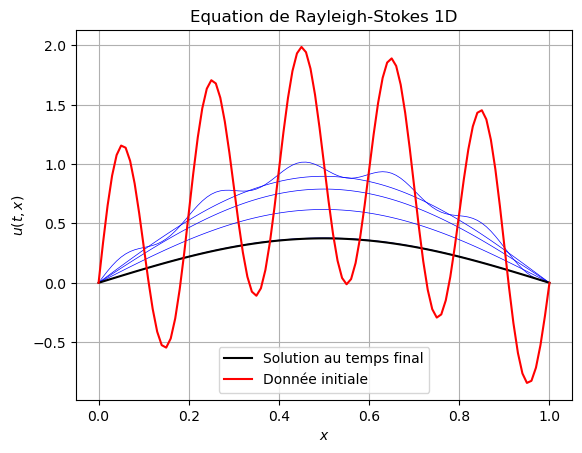
\includegraphics[width=\textwidth]{images/stabilite/alpha_dix_moins_5.png}
        \caption{$\alpha=10^{-5}$}
    \end{subfigure}
    \hfill
    \begin{subfigure}{0.32\textwidth}
        \centering
        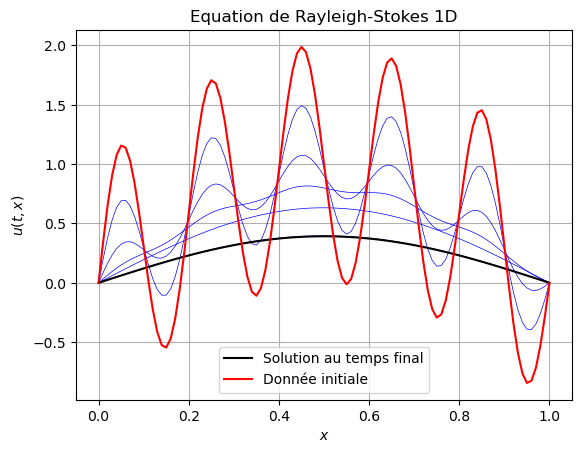
\includegraphics[width=\textwidth]{images/stabilite/alpha_dix_moins_2.png}
        \caption{$\alpha=5\times 10^{-3}$}
    \end{subfigure}
    \hfill
    \begin{subfigure}{0.32\textwidth}
        \centering
        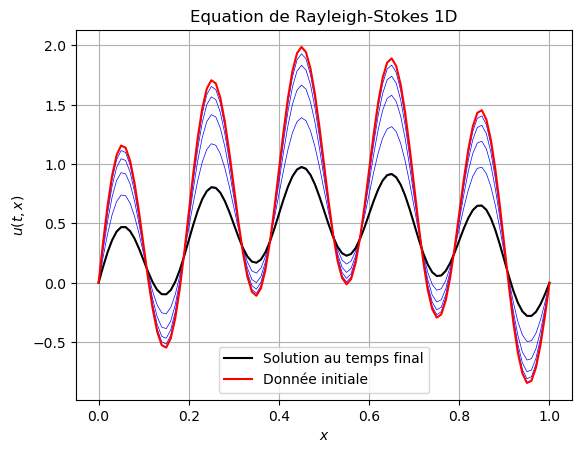
\includegraphics[width=\textwidth]{images/stabilite/alpha_dix_moins_1.png}
        \caption{$\alpha=10^{-1}$}
    \end{subfigure}
    \caption{Comportement des hautes fréquences en fonction de $\alpha$}
    \label{fig:stabilite_alpha}
\end{figure}
Sur la figure (a), on a $\alpha \ll \nu \Delta t$ et les hautes fréquences sont immédiatement amorties. Sur la figure (b), on a $\alpha \sim \nu \Delta t$, les hautes fréquences sont amorties mais cela prend plus de temps. Sur la figure (c), $\alpha \gg \nu \Delta t$, les hautes fréquences sont conservées. Cette exemple illustre parfaitement l'analyse précédente.

\subsubsection{Erreur globale et convergence}
Le schéma est consistant d'ordre un en temps et deux en espace, il est également stable en norme $L^2$, par conséquent la solution numérique converge vers la solution exacte. De plus, l'erreur globale est en $O(\Delta t +h^2)$.

\subsubsection{Conditionnement}
On va étudier le conditionnement de la matrice $A:=I-(\nu\Delta t+\alpha)\Delta_h$ pour mettre en évidence son impact dans la stabilisation du comportement numérique. La matrice est définie par
\begin{eqnarray*}
    I - (\nu\Delta t +\alpha)\Delta_h = \begin{pmatrix}
        1+2\frac{\nu \Delta t+\alpha}{h^2} & -\frac{\nu\Delta t + \alpha}{h^2} & 0  & \cdots & 0 \\
       -\frac{\nu\Delta t + \alpha}{h^2} & 1+2\frac{\nu \Delta t+\alpha}{h^2} & -\frac{\nu\Delta t + \alpha}{h^2}  & \ddots & \vdots \\
        0 & \ddots & \ddots & \ddots &  0 \\
        \vdots & \ddots & \ddots & \ddots &  -\frac{\nu\Delta t + \alpha}{h^2} \\
        0 & \cdots &  0 & -\frac{\nu\Delta t + \alpha}{h^2} & 1+2\frac{\nu \Delta t+\alpha}{h^2}
    \end{pmatrix}
\end{eqnarray*}
On va utiliser le théorème de Gerschgorin pour connaître le spectre de $A$. Les disques de Gerschgorin sont 
\begin{eqnarray*}
    D_1 = D_m &=& B\bigg(1+2\frac{\nu\Delta t+\alpha}{h^2}, \ \frac{\nu\Delta t+\alpha}{h^2}\bigg) \\
    \forall i \in \{2,\dots,m-1\}, \ D_i &=& B\bigg(1+2\frac{\nu\Delta t+\alpha}{h^2}, \ 2\frac{\nu\Delta t+\alpha}{h^2}\bigg)
\end{eqnarray*}
où $B(x, r)$ désigne la boule de centre $x$ et de rayon $r$ pour la norme euclidienne. Par le théorème de Gerschgorin, on a 
\begin{equation*}
    \mathrm{Sp}(A) \subset \bigcup_{i=1}^m D_i = B\bigg(1+2\frac{\nu\Delta t+\alpha}{h^2}, \ 2\frac{\nu\Delta t+\alpha}{h^2}\bigg)
\end{equation*}
or, $A$ est symétrique, donc diagonalisable à valeurs propres réelles. Ainsi, 
\begin{equation*}
    \mathrm{Sp}(A) \subset  \Big[1, \ 1+4\frac{\nu\Delta t+\alpha}{h^2}\Big]
\end{equation*}
De plus, $A$ est irréductible car son graphe est connexe donc si $\lambda$ est une valeur propre de $A$, on a 
\begin{eqnarray*}
    \lambda \in \bigcup_{i=1}^m \partial D_i &\Longrightarrow& \lambda \in 
    \bigcap_{i=1}^m \partial D_i = \emptyset
\end{eqnarray*}
On peut donc affiner notre localisation du spectre de $A$
\begin{equation*}
    \mathrm{Sp}(A) \subset \  \Big]1, \ 1+4\frac{\nu\Delta t+\alpha}{h^2}\Big[ \ \setminus \Big\{1+\frac{\nu\Delta t+\alpha}{h^2}, 1+3\frac{\nu\Delta t+\alpha}{h^2} \Big\}
\end{equation*}
On en déduit 
\begin{eqnarray*}
    \lambda_1 := \min_{\lambda \in \mathrm{Sp}(A)} \lambda > 1 \ \ \ &\text{ et }& \ \ \ \lambda_m :=\max_{\lambda \in \mathrm{Sp}(A)} \lambda < 1+4\frac{\nu\Delta t+\alpha}{h^2}
\end{eqnarray*}
Finalement,
\begin{equation*}
    \mathrm{cond}(A) = \frac{\lambda_m}{\lambda_1} < 1+4\frac{\nu \Delta t +\alpha}{h^2}
\end{equation*}
Donc, si on choisit $\alpha$ et $\Delta t$ tels que $\nu \Delta t \ll \alpha$ alors 
\begin{equation*}
    \mathrm{cond}(A) \leq 1 + \frac{\alpha}{h^2}
\end{equation*}
Le conditionnement de $A$ devient indépendant de $\Delta t$ ce qui permet de faire varier librement le pas de temps sans influer sur la stabilité numérique du schéma.
\begin{remark}
     Si on veut que le conditionnement de la matrice $A$ soit indépendant du choix de $\Delta t$ on doit choisir $\nu \Delta t \ll \alpha$, or on a vu lors de l'étude de la stabilité du schéma que pour avoir un effet de filtre passe-bas on devait choisir $\nu \Delta t \gg \alpha$. En pratique, on privilégiera la propriété de filtre passe-bas tout en faisant attention à ce que cela ne limite pas notre façon de résoudre le système linéaire $AX=Y$.
\end{remark}

\subsection{Comparaison avec l'équation de la chaleur}
Dans cette section, on veut comparer le schéma d'Euler implicite entre l'équation de Rayleigh-Stokes et l'équation de la chaleur. On considère les problèmes aux limites suivants
\begin{itemize}
    \item Problème aux limites pour l'équation de Rayleigh-Stokes
    \begin{equation*}
        \begin{cases}
            \partial_tu(t,x) - \nu\partial_{xx} u(t,x) - \alpha\partial_{xx} \big(\partial_t u(t,x)\big) = 0 & \forall (t,x) \in \ ]0, 1[ \ \times \ ]0,1[  \\
            u(0,x) = u_0(x) = \sin{(\pi x)} & \forall x \in \ ]0,1[ \\
            u(t, 0) = u(t,1) = 0 & \forall t \in \ ]0,1[
        \end{cases}
    \end{equation*}
    La solution de ce problème est donnée par 
    \begin{equation}\label{compRSchaleur_solRS}
        u_{\text{RS}}(t,x) = \sin{(\pi x)}\exp{\Big( -\frac{\nu \pi^2}{1+\alpha \pi^2}t\Big)}
    \end{equation}
    \item Problème aux limites pour l'équation de la chaleur
    \begin{equation*}
        \begin{cases}
            \partial_tu(t,x) - \nu\partial_{xx} u(t,x) = 0 & \forall (t,x) \in \ ]0,1[ \ \times \ ]0,1[  \\
            u(0,x) = u_0(x)=\sin{(\pi x)} & \forall x \in \ ]0,1[ \\
            u(t, 0) = u(t,1) = 0 & \forall t \in \ ]0,1[
        \end{cases}
    \end{equation*}
    La solution de ce problème est donnée par 
    \begin{equation}\label{compRSchaleur_solchaleur}
        u_{\text{chal}}(t,x) = \sin{(\pi x)}\exp{(-\nu \pi^2t)}
    \end{equation}
\end{itemize}
L'objectif ici est d'observer l'influence du paramètre $\alpha$ sur la dissipation de l'énergie cinétique et de comparer ce phénomène avec l'équation de la chaleur (cas $\alpha=0$). Pour nos simulations, on choisit $\nu = 0.1$, et $h=\Delta t = \dfrac{1}{100}$. La simulation pour l'équation de la chaleur donne le résultat suivant
\begin{figure}[!ht]
    \centering
    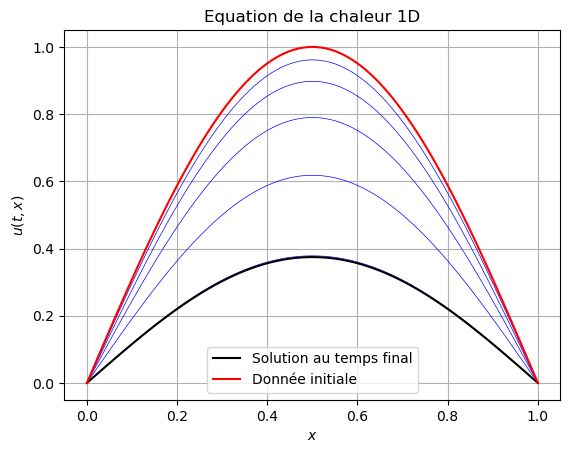
\includegraphics[width=0.5\linewidth]{images/comparaison_chaleur/eq_chaleur.png}
    \caption{\'Equation de la chaleur $1$D pour l'évolution temporelle du profil de vitesse $u(t,x)$ pour un mode sinusoïdal}
    \label{fig:eqchaleur}
\end{figure}
\\
Pour comparer à l'équation de Rayleigh-Stokes, on choisit $\alpha \in \{5\times 10^{-1}, 5 \times 10^{-2}, 5 \times 10^{-4}\}$, voici les résultats des simulations
\begin{figure}[!ht]
    \centering
    \begin{subfigure}{0.32\textwidth}
        \centering
        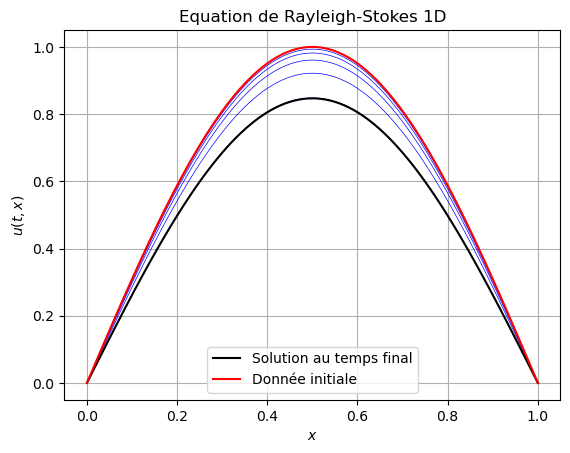
\includegraphics[width=\textwidth]{images/comparaison_chaleur/eq_RS_alpha1.png}
        \caption{$\alpha=5\times 10^{-1}$}
    \end{subfigure}
    \hfill
    \begin{subfigure}{0.32\textwidth}
        \centering
        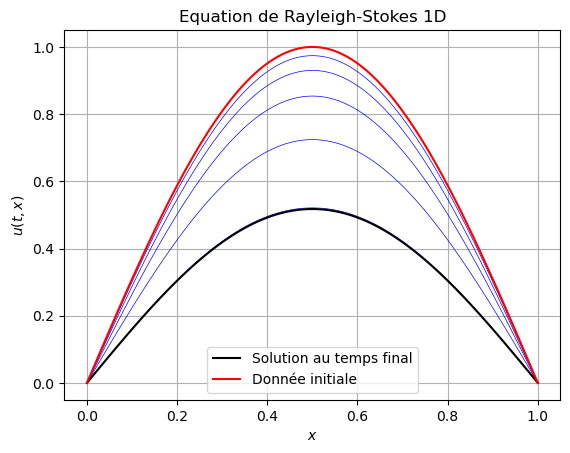
\includegraphics[width=\textwidth]{images/comparaison_chaleur/eq_RS_alpha2.png}
        \caption{$\alpha=5\times 10^{-2}$}
    \end{subfigure}
    \hfill
    \begin{subfigure}{0.32\textwidth}
        \centering
        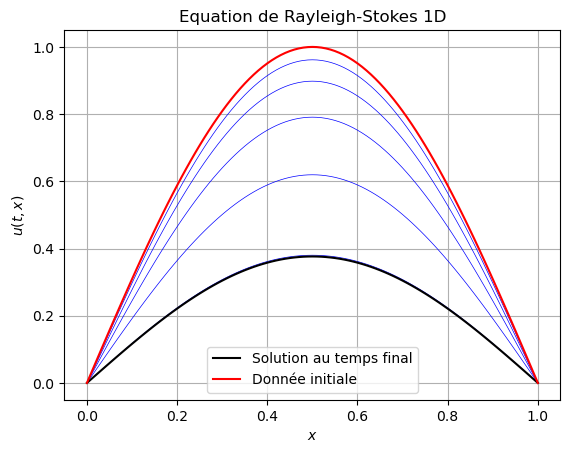
\includegraphics[width=\textwidth]{images/comparaison_chaleur/eq_RS_alpha3.png}
        \caption{$\alpha=5 \times 10^{-4}$}
    \end{subfigure}
    \caption{Influence du paramètre $\alpha$ sur la dissipation de l'énergie pour l'équation de Rayleigh-Stokes $1$D}
    \label{fig:comparaisonchaleurRS}
\end{figure}
\\
On remarque que sur la figure \ref{fig:eqchaleur}, le profil sinusoïdal est très rapidement amorti. Physiquement, c'est une diffusion classique du fluide, le mouvement du fluide va s'arrêter rapidement. Analytiquement, la solution est donnée par \eqref{compRSchaleur_solchaleur} avec 
\begin{equation*}
    \nu \pi^2 \approx 0.99
\end{equation*}
on a une décroissance exponentielle ce qui explique l'amortissement rapide du profil sinusoïdal.
Sur les figures \ref{fig:comparaisonchaleurRS}, on observe plusieurs cas en fonction de la valeur du paramètre $\alpha$. Le paramètre $\alpha$ est un paramètre de viscoélasticité du fluide, il va donc agir comme une contrainte supplémentaire sur le fluide et ralentir plus ou moins la diffusion. 
Sur la figure (a) de \ref{fig:comparaisonchaleurRS}, $\alpha$ est grand (dans le sens de l'ordre de $\nu$) et on observe que le profil sinusoïdal n'est presque pas amorti. La diffusion est donc ralentie par le paramètre $\alpha$. Si on regarde la solution \eqref{compRSchaleur_solRS} dans cette configuration, on a 
\begin{equation*}
    \frac{\nu \pi^2}{1+\alpha \pi^2} \approx 0.17
\end{equation*}
La décroissance exponentielle est fortement ralentie par la présence du terme $\alpha$ grand.
Sur la figure (b) de \ref{fig:comparaisonchaleurRS}, $\alpha$ est plus petit, le profil sinusoïdal est amorti mais toujours plus lentement que pour l'équation de la chaleur. Ici, on a 
\begin{equation*}
    \frac{\nu \pi^2}{1+\alpha \pi^2} \approx 0.66
\end{equation*}
On retrouve à nouveau l'influence du paramètre $\alpha$ sur la décroissance exponentielle du profil.
Enfin sur la figure (c) de \ref{fig:comparaisonchaleurRS}, $\alpha$ est négligeable devant $\nu$ et on retrouve un amortissement du profil comme pour l'équation de la chaleur \ref{fig:eqchaleur}. Ici, on a
\begin{equation*}
    \frac{\nu \pi^2}{1+\alpha \pi^2} \approx 0.98
\end{equation*}
La contrainte physique liée au paramètre $\alpha$ est très faible, c'est donc le caractère diffusif qui va prendre le dessus.
    
\subsection{Quelques exemples}
\subsubsection{La fonction indicatrice}
Pour ce premier cas on s’intéresse au problème suivant:
   \begin{equation*}
        \begin{cases}
            \partial_tu(t,x) - \nu\partial_{xx} u(t,x) - \alpha\partial_{xx} \big(\partial_t u(t,x)\big) = 0 & \forall (t,x) \in \ ]0, T[ \ \times \ ]0,L[  \\
            u(0,x) = u_0(x) = \mathds{1}_{\left[\tfrac{L}{4},\tfrac{3L}{4}\right]}(x) & \forall x \in \ ]0,L[ \\
            u(t, 0) = u(t,L) = 0 & \forall t \in \ ]0,T[
        \end{cases}
    \end{equation*}
Après une décomposition en série de Fourier la solution est donnée par
\begin{eqnarray*}
    u(t,x) = \sum_{k=1}^{N} c_k \exp\left(-\frac{\nu\lambda_k}{1+\alpha\lambda_k}\,t\right)\sin\left(\frac{k\pi x}{L}\right)
\end{eqnarray*}
avec 
\begin{equation*}
    c_k = \frac{2}{k\pi}\left(\cos(\frac{k\pi}{4}) -\cos(\frac{3k\pi}{4})\right)
\end{equation*}
Cette décomposition repose sur le fait que notre fonction initial peut s'écrire comme une série composé de sinus sur $[0,L]$
\begin{eqnarray*}
    u_0(x) = \sum_{k=1}^{\infty} c_k \sin\left(\frac{k\pi x}{L}\right)
\end{eqnarray*}
En multipliant par $\sin\Big(\dfrac{j\pi x}{L}\Big)$ de chaque côté et intégrant sur $[0,L]$ cela nous permet d'identifier $c_k$. \\
On résout numériquement le problème en posant $N = 200$, $L=10$ et $T=20$. Pour les paramètre de l'équation de Rayleigh-Stokes on choisi $\nu = 0.4$ et $\alpha=0.5$ Cela va nous permettre d'étudier comment varie notre solution initial et quels sont les effets du paramètre $\alpha$.  
\begin{figure}[!ht]
    \centering
    \begin{subfigure}{0.48\textwidth}
        \centering
        \includegraphics[width=\textwidth]{images/Exemples/Indicatrice/resolution_indicatrice.png}
        \caption{Évolution de la solution}
    \end{subfigure}
    \hfill
    \begin{subfigure}{0.48\textwidth}
        \centering
        \includegraphics[width=\textwidth]{images/Exemples/Indicatrice/comparaison_final_theorique_indicatrice.png}
        \caption{Comparaison solution finale/théorique}
    \end{subfigure}
    \caption{ Résolution de l'équation de Rayleigh-Stokes $1$D}
    \label{fig:Exemples_RS_Stokes_indicatrice}
\end{figure}
\begin{figure}[H]
    \centering
    \includegraphics[width=\linewidth]{images/Exemples/Indicatrice/comparaison alpha indicatrice.png}
    \caption{Comparaison en fonction de alpha}
    \label{Indicatrice_comparaisons des alpha}
\end{figure}
On observe sur la figure \eqref{fig:Exemples_RS_Stokes_indicatrice} que la solution initial discontinue est rapidement lissé et amorti cela correspond bien aux résultats observés précédemment.

La figure \eqref{Indicatrice_comparaisons des alpha} illustre l'influence du paramètre
$\alpha$ : pour $\alpha$ grand, le fluide résiste davantage au changement
et conserve plus longtemps la mémoire de son état initial.

\subsubsection{Problème de Stokes impulsif, démarrage brusque d’une paroi}
On va maintenant simuler la réponse d'un fluide à l'accélération d'une paroi. On se place dans un canal de largeur $L=1$ au temps initial $t=0$. On suppose qu'au temps initial le fluide est au repos. On impose ensuite une vitesse constante $U_0$ sur le bord $x=0$, ici on prendra $U_0=10$. Le problème s'écrit alors:
\begin{equation*}
    \begin{cases}
        \partial_tu(t,x) - \nu\partial_{xx} u(t,x) - \alpha\partial_{xx} \big(\partial_t u(t,x)\big) = 0 & \forall (t,x) \in \ ]0, 5[ \ \times \ ]0,1[  \\
        u(0,x) = u_0(x) = 0 & \forall x \in \ ]0,1[ \\
        u(t,1) = 0 & \forall t \in \ ]0,5[ \\
        u(t,0) = U_0 & \forall t \in \ ]0,5[
    \end{cases}
\end{equation*}
Le problème n'ayant plus des conditions de Dirichlet homogène il faut faire un relèvement. On pose $u = \Tilde{u} + g$ avec $\Tilde{u} \in H^1_0([0,1])$  et $g(x) = U_0 \Big(1 - \dfrac{x}{L}\Big)$ de sorte que $g(1)=0$ et $g(0) = U_0$.
La formulation variationnelle reste la même que dans le cas homogène, il faut juste prendre en compte la fonction $g$ dans les conditions initiales et dans la solution du problème. On obtient le résultat suivant
\begin{figure}[!ht]
    \centering
    \begin{subfigure}{0.32\textwidth}
        \centering
        \includegraphics[width=\textwidth]{images/Exemples/Plaque en mouvement/RS_EI_plaque_1.png}
        \caption{$\alpha=0.1$}
    \end{subfigure}
    \hfill
    \begin{subfigure}{0.32\textwidth}
        \centering
        \includegraphics[width=\textwidth]{images/Exemples/Plaque en mouvement/RS_EI_plaque_2.png}
        \caption{$\alpha=0.5$}
    \end{subfigure}
    \hfill
    \begin{subfigure}{0.32\textwidth}
        \centering
        \includegraphics[width=\textwidth]{images/Exemples/Plaque en mouvement/RS_EI_plaque_3.png}
        \caption{$\alpha=0.9$}
    \end{subfigure}
    \caption{Influence du paramètre $\alpha$ sur la résistance du fluide face à la condition initiale pour l'équation de Rayleigh-Stokes $1$D}
    \label{fig:Exemples_RS_Stokes_impulsif}
\end{figure} \\
On peut remarquer que sur les 3 cas précédents le terme en $\alpha$ joue un rôle sur l'accélération de la vitesse. Si $\alpha$ est petit alors le profil du fluide rejoint rapidement le profil de Couette alors que pour une grande valeur on va avoir besoin de beaucoup plus de temps pour rejoindre le profil final. Le terme $\alpha$ joue un rôle de \og mémoire \fg{}, le fluide résiste au changement pour garder son état initial. \\
Ce genre de propriétés s'avèrent importantes dans le monde industriel où ce genre de mouvement peu avoir lieu lors du démarrage de système de pompage d'un fluide complexe. Si le fluide subit une accélération rapide il faut être capable de savoir à quel point il résistera car s'il est très visqueux cela entraînera des contraintes de cisaillement élevés qui pourraient abîmer les parois de la machine.

\subsubsection{Régime forcé et analyse du déphasage viscoélastique}
%T = 4 
%v = 0.4
%alpha = 0.6
%L = 10
%Nx = 500
%omega = 0.5 
%A = 2 
%alpha1 = (np.pi / L)**2
%phi = np.arctan2(gamma * (1 + alpha * alpha1), v * alpha1)
Ce cas test étudie la réponse du fluide à une sollicitation externe périodique. Contrairement aux tests précédents, ici il y a un terme source et nous regardons l’établissement d’un cycle limite stationnaire, mais pas immobile. L'équation de Rayleigh-Stokes s'écrit. 
\begin{eqnarray}\label{RS_exemple_dephasage}
    \partial_tu(t,x) - \nu \partial_{xx}u(t,x) - \alpha \partial_{txx}u(t,x) = A \sin(\omega t)\sin\Big(\frac{\pi x}{L}\Big)
\end{eqnarray}
Le paramètre $A$ correspond à l'amplitude et $\omega$ à la pulsation. On pose d'abord $L= 10, \ A=5 \text{ et } \omega = 0.7$. On cherche à résoudre le problème jusqu'au temps $T=4$ pour $\nu = 0.4 \text{ et } \alpha=0.5$.
Calculons la solution exacte pour comparer avec notre schéma. On procède par séparation de variable et on cherche une solution de la même forme
\begin{eqnarray*}
    u(t,x) = v(t) \sin\Big(\frac{\pi x}{L}\Big)
\end{eqnarray*}
En calculant les dérivées partielles et en notant $\lambda_1 := \Big(\dfrac{\pi}{L} \Big)^2$ on peut réécrire \eqref{RS_exemple_dephasage}
\begin{equation*}
    v'(t) \sin\Big(\frac{\pi x}{L}\Big) + \nu \lambda_1 v(t)\sin\Big(\frac{\pi x}{L}\Big) + \alpha \lambda_1 v'(t)\sin\Big(\frac{\pi x}{L}\Big) = A\sin(\omega t)\sin\Big(\frac{\pi x}{L}\Big)
\end{equation*}
Comme pour tout $x \in \ ]0,L[$, $\sin\Big(\dfrac{\pi x}{L}\Big) \neq 0$, on peut simplifier et ainsi obtenir
\begin{equation*}
    (1 + \alpha \lambda_1)v'(t) + \nu \lambda_1v(t) = A \sin(\omega t)
\end{equation*}
On cherche une solution particulière de cette EDO sous la même forme que le second membre
\begin{equation*}
    v(t) = P \sin(\omega t) + Q\cos(\omega t) \ \ \ \ \ \text{ où } P, Q \in \bbR
\end{equation*}
Alors 
\begin{equation*}
    v'(t) = \omega P \cos(\omega t) - \omega Q\sin(\omega t)
\end{equation*}
On trouve alors $P = \dfrac{\nu \lambda_1 A}{D}$ et $Q= - \dfrac{(1 + \alpha \lambda_1)\omega A}{D}$ où $D := (1+\alpha \lambda_1) + (\nu \lambda_1)^2$.
Puis, en utilisant la propriété trigonométrique
\begin{eqnarray} \label{trigo_equation_exemple}
    \sin(\omega t - \varphi) = \cos(\varphi)\sin(\omega t) - \sin(\varphi)\cos(\omega t)
\end{eqnarray}
on identifie 
\begin{eqnarray*}
    \frac{\nu \lambda_1 A}{D} = \cos(\varphi) \ \ \  &\text{ et }& \ \ \ \frac{(1 + \alpha \lambda_1)\omega A}{D}= \sin(\varphi)
\end{eqnarray*}
d'où 
\begin{equation*}
    \varphi= \arctan \bigg(\frac{(1+\alpha \lambda_1) \omega}{\nu \lambda_1}\bigg)
\end{equation*}
De plus en multipliant \eqref{trigo_equation_exemple} par $U(\omega)$ on trouve que $U$ doit vérifier $U(\omega) = \sqrt{P^2 + Q^2}$. Finalement on obtient une solution 
\begin{equation*}
    v(t) = C \exp{\Big(-\frac{\nu \lambda_1}{1+ \alpha \lambda_1}t\Big)} + U(\omega)\sin(\omega t-\varphi) \ \ \ \ \ \text{ où } C \in \bbR
\end{equation*}
En supposant que le fluide est au repos à l'état initial, c'est-à-dire $u_0 = 0$ on trouve 
\begin{equation*}
    C = -U(\omega) \sin(-\varphi) = U(\omega) \sin(\varphi)
\end{equation*}
Donc $v(t)$ s'écrit
\begin{equation*}
    v(t) = U(\omega) \sin(\varphi) \exp{\Big(-\frac{\nu \lambda_1}{1+ \alpha \lambda_1}t\Big)} + U(\omega)\sin(\omega t-\varphi)
\end{equation*}
Ce qui nous permet d'écrire la solution
\begin{equation*}
    u(t,x) = \bigg(U(\omega) \sin(\varphi) \exp{\Big(-\frac{\nu \lambda_1}{1+ \alpha \lambda_1}t\Big)} + U(\omega)\sin(\omega t-\varphi) \bigg) \sin\Big(\frac{\pi x}{L}\Big)
\end{equation*}
En temps long on remarque que l'exponentielle tend vers $0$. On simplifiera alors la solution en 
\begin{equation*}
    u(t,x) = U(\omega)\sin(\omega t-\varphi)  \sin\Big(\frac{\pi x}{L}\Big)
\end{equation*}
On peut alors étudier cette équation en fonction des paramètres $\alpha$ et $\omega$. La résolution numérique donne les résultats suivant:
\begin{figure}[H]
    \centering
    \begin{subfigure}{0.47\textwidth}
        \centering
        \includegraphics[width=\textwidth]{images/Exemples/Dephasage viscoelastique/RS_dephasage.png}
        \caption{$\alpha=0.5$}
    \end{subfigure}
    \hfill
    \begin{subfigure}{0.47\textwidth}
        \centering
        \includegraphics[width=\textwidth]{images/Exemples/Dephasage viscoelastique/RS_dephasage final.png}
        \caption{$\alpha=0.5$}
    \end{subfigure}
    \hfill
    \caption{Analyse d'un régime forcé pour l'équation de Rayleigh-Stokes $1$D}
    \label{fig:Exemples_RS_Stokes_régime_forcé}
\end{figure} 
\begin{figure}[H]
    \centering
    \begin{subfigure}{0.47\textwidth}
        \centering
        \includegraphics[width=\textwidth]{images/Exemples/Dephasage viscoelastique/RS_convergence_temps_dephasage.png}
        \caption{Ordre de convergence}
    \end{subfigure}
    \hfill
    \begin{subfigure}{0.47\textwidth}
        \centering
        \includegraphics[width=\textwidth]{images/Exemples/Dephasage viscoelastique/Amplitude de la reponse.png}
        \caption{Variation théorique}
    \end{subfigure}
    \hfill
    \caption{Étude de la convergence en temps et de l'évolution de l’amplitude pour l'équation de Rayleigh-Stokes $1$D} \label{fig:Exemples_RS_Stokes_régime_forcé_comparaison_final}
\end{figure} 
\begin{figure}[H]
    \centering
    \begin{subfigure}{0.47\textwidth}
        \centering
        \includegraphics[width=\textwidth]{images/Exemples/Dephasage viscoelastique/Amplitude alpha.png}
        \caption{Évolution de l'amplitude en fonction de $\alpha$ }
    \end{subfigure}
    \hfill
    \begin{subfigure}{0.47\textwidth}
        \centering
        \includegraphics[width=\textwidth]{images/Exemples/Dephasage viscoelastique/Amplitude_omega.png}
        \caption{Amplitude numérique en fonction de $\omega$}
    \end{subfigure}
    \hfill
    \caption{Étude de l’amplitude pour l'équation de Rayleigh-Stokes $1$D}
    \label{fig:Exemples_RS_Stokes_régime_forcé_amplitude}
\end{figure} 

Sur les dernières images on a mis en évidence que le paramètre $\omega$ influe fortement sur l'évolution de l'amplitude de la vitesse du fluide, contrairement au paramètre $\alpha$ qui lui à un effet plus modéré. Ce sont des propriétés similaires de filtres passe bas que nous avions trouvé précédemment. Plus $\omega$ est grand plus la pulsation est importante et donc la fréquence est élevée. Or l'amplitude est plus atténuée, les hautes fréquences sont filtrées.
\newpage
\subsection{Un autre schéma}
Dans cette section, on va chercher à augmenter la précision en temps de notre schéma, pour ça on s'intéresse au schéma de Crank-Nicolson. Pour ça, on repart de l'équation \eqref{schema_semi_discret}, on intègre entre deux instants $t_n$, $t_{n+1}$ et on utilise cette fois la méthode des trapèzes pour approximer les intégrales. Ce qui nous donne après avoir divisé par $\Delta t$
\begin{eqnarray}\label{schemaCN1}
    \frac{u_i^{n+1}-u_i^n}{\Delta t} &-& \frac{\nu}{2} \bigg( \frac{u_{i-1}^{n+1}-2u_i^{n+1}+ u_{i+1}^{n+1}}{h^2} + \frac{u_{i-1}^{n}-2u_i^{n}+u_{i+1}^{n}}{h^2} \bigg) \\
    &-& \frac{\alpha}{\Delta t}\bigg( \frac{u_{i-1}^{n+1}-2u_i^{n+1}+u_{i+1}^{n+1}}{h^2} 
    -\frac{u_{i-1}^{n}-2u_i^{n}+u_{i+1}^{n}}{h^2}\bigg) = f_i \nonumber
\end{eqnarray}
%Puisque nous avons réalisé notre étude à partir du schéma d'Euler implicite, il est facile de retrouver plusieurs propriétés importantes du schéma de Crank-Nicolson qui est construit en faisant un moyenne du schéma d'Euler implicite et explicite. \\
%Le schéma d'Euler implicite donnait :
%\begin{eqnarray*}
%    \frac{U^{n+1} - U^n}{\Delta t} - \nu \Delta _h U^{n+1} - \alpha\bigg(\frac{\Delta_h U^{n+1} - \Delta_h U^n}{\Delta t} \bigg) = F
%\end{eqnarray*}
%Le schéma d'Euler explicite s'écrit alors simplement :
%\begin{eqnarray*}
%    \frac{U^{n+1} - U^n}{\Delta t} - \nu \Delta _h U^{n} - \alpha\bigg(\frac{\Delta_h U^{n+1} - \Delta_h U^n}{\Delta t} \bigg) = F
%\end{eqnarray*}
Avec les notations introduites dans la section sur le schéma d'Euler implicite, on peut réécrire l'équation précédente de la façon suivant
\begin{equation*}
    \frac{U^{n+1} - U^n}{\Delta t} - \frac{\nu}{2} \big(\Delta _h U^{n+1}-\Delta_hU^n\big) - \alpha\bigg(\frac{\Delta_h U^{n+1} - \Delta_h U^n}{\Delta t} \bigg) = F
\end{equation*}
Finalement, en isolant l'inconnue au temps $n+1$ et au temps $n$ on peut écrire le système final
\begin{eqnarray*}
    \Big(I - \Big( \frac{\nu \Delta t}{2} + \alpha \Big)\Delta_h\Big)  U^{n+1} = \Big(I + \Big(\frac{\nu \Delta t}{2} - \alpha\Big) \Delta_h\Big) U^n + \Delta t F
\end{eqnarray*}

\subsubsection{Consistance}
Le schéma de Crank-Nicolson est consistant d'ordre deux en temps et en espace. Comme dans la section sur le schéma d'Euler implicite on montre cela par un calcul avec des développements limités. On pose
\begin{eqnarray*}
    A &:=& \frac{u(t+\Delta t,x)-u(t,x)}{\Delta t} \\
    B &:=& \frac{\nu}{2}\bigg(\frac{u(t+\Delta t,x-h)-2u(t+\Delta t, x)+ u(t+\Delta t, x+h)}{h^2} \\
    &+& \frac{u(t,x-h)-2u(t, x) + u(t, x+h)}{h^2}\bigg) \\
    C &:=&\frac{\alpha}{\Delta t}\bigg(\frac{u(t+\Delta t,x-h)-2u(t+\Delta t, x) + u(t+\Delta t, x+h)}{h^2} \\
    &-&\frac{u(t,x-h)-2u(t, x)+u(t, x+h)}{h^2}\bigg) \\
    \calL_hu(t,x) &=& A - B - C 
\end{eqnarray*}
Comparé au schéma d'Euler implicite, seul le terme $B$ est modifié, on utilise donc nos calculs précédents et on effectue le développement limité du terme supplémentaire dans l'expression de $B$. Ce qui donne
\begin{eqnarray*}
    A &=& \partial_{t}u(t,x) - \frac{\Delta t}{2} \partial_{tt}u(t,x) + O(\Delta t^2) \\
    B &=&  \frac{\nu}{2} \Big(\partial_{xx}u(t,x) + \Delta t \partial_{xxt}u(t,x) + \frac{h^2}{12} \partial_{xxxx}u(t,x) + O(\Delta t^2+h^3)\Big) \\
    &+& \frac{\nu}{2} \Big(\partial_{xx}u(t,x) + \frac{h^2}{12} \partial_{xxxx}u(t,x) + O(h^3)\Big) \\
    C &=& \alpha\Big(\partial_{xxt}u(t,x) + \frac{h^2}{12}\partial_{xxxxt}u(t,x) - \frac{\Delta t}{2}\partial_{xxtt}u(t,x) - \frac{h^2\Delta t}{24}\partial_{xxxxtt}u(t,x) \\
    &+& O(\Delta t^2 + h^3)\Big)   
\end{eqnarray*}
D'où 
\begin{eqnarray*}
    \calL_hu -\calL u &=& -\frac{\Delta t}{2}\partial_{tt}u + \nu\frac{\Delta t }{2} \partial_{xxt}u+ \alpha\frac{\Delta t }{2} \partial_{xxtt}u  + O(\Delta t^2 + h^2)
\end{eqnarray*}
On utilise notre EDP
\begin{eqnarray*}
    \partial_tu = \nu \partial_{xx}u + \alpha \partial_{xxt}u 
    & \Longrightarrow& 
    \partial_{tt}u = \nu \partial_{xxt}u + \alpha \partial_{xxtt}u
\end{eqnarray*}
L'erreur de troncature se simplifie alors en
\begin{eqnarray*}
    \calL_hu -\calL u &=& -\frac{\Delta t}{2}(\nu \partial_{xxt}u + \alpha \partial_{xxtt}u) + \nu\frac{\Delta t }{2} \partial_{xxt}u+ \alpha\frac{\Delta t }{2} \partial_{xxtt}u  + O(\Delta t^2 + h^2) \\
    &=& O(\Delta t^2 + h^2)
\end{eqnarray*}
Le schéma est bien d'ordre deux en temps et en espace.

\subsubsection{Stabilité}
On utilise les notations introduites à la section \ref{Stabilité_EI}. Tout comme le schéma d'Euler implicite ce schéma vérifie les conditions de stabilité de Von Neumann. En effet, on part de \eqref{schemaCN1} et en réalisant exactement les mêmes calculs qu'à la section \eqref{Stabilité_EI}, on obtient
\begin{eqnarray*}
    \Big(1+\Big(\alpha +\frac{\nu \Delta t}{2}\Big) \frac{4}{h^2}\sin^2(\pi k h)\Big)\hat{u}^{n+1}(k) &=& \Big(1+\Big(\alpha - \frac{\nu \Delta t}{2}\Big) \frac{4}{h^2}\sin^2(\pi kh)\Big)\hat{u}^{n}(k)
\end{eqnarray*}
Le facteur d'amplification de ce schéma s'écrit alors
\begin{eqnarray*}
    \mathscr{A}(k \ ; \Delta t ,h) &=& \frac{1+\Big(\alpha - \dfrac{\nu \Delta t}{2}\Big) \dfrac{4}{h^2}\sin^2(\pi kh)}{1+\Big(\alpha +\dfrac{\nu \Delta t}{2}\Big) \dfrac{4}{h^2}\sin^2(\pi kh) }
\end{eqnarray*}
On pose $a=\alpha \dfrac{4}{h^2}\sin^2(\pi kh)$ et $b=\dfrac{\nu \Delta t}{2}\dfrac{4}{h^2}\sin^2(\pi kh)$, comme $\alpha, \ \nu, \ h, \ \Delta t >0$ on a $a, \ b >0$. Le facteur d'amplification s'écrit alors
\begin{eqnarray*}
    \scrA(k \ ; \Delta t ,h) &=& \frac{1+a-b}{1+a+b}
\end{eqnarray*}
on cherche à savoir si $|\scrA(k \ ; \Delta t ,h)| \leq 1$, donc si 
\begin{eqnarray*}
    \bigg|\frac{1+a-b}{1+a+b}\bigg| \leq 1 &\Longrightarrow& |1+a-b| \leq 1+a+b
\end{eqnarray*}
ce qui nous donne deux conditions
\begin{eqnarray*}
    1+a-b < 1+a+b \ \ \ &\text{ ou }& \ \ \ -1-a-b < 1+a-b \\
    0 < 2b \ \ \ &\text{ ou }& \ \ \ 0 < 2(1+a)
\end{eqnarray*}
ces deux conditions sont toujours vérifiées donc,
\begin{eqnarray*}
    \sup_{k \in \mathbb{Z}} \ |\mathscr{A}(k \ ; \Delta t ,h)| &\leq& 1
\end{eqnarray*}
Le schéma est donc stable en temps long et inconditionnellement stable en norme $L^2$.
On remarquera que contrairement aux schéma d'Euler implicite il est possible d'obtenir un facteur d'amplification négatif avec $\alpha < \dfrac{\nu \Delta t}{2}$.
% A voir ce que ça veut dire j'ai pas creusé plus. On devrait demander à Marche.

\subsubsection{Erreur globale et convergence}
Le schéma est consistant d'ordre deux en temps et en espace, il est également stable en norme $L^2$, par conséquent la solution numérique converge vers la solution exacte. De plus, l'erreur globale est en $O(\Delta t^2 +h^2)$.

\subsubsection{Comparaison avec le schéma d'Euler implicite}
On va implémenter un cas simple afin de mettre en évidence la différence de précision en temps du schéma d'Euler implicite et de celui de Crank-Nicolson. Pour ça, on choisit $L=\nu = T = 1$, $\alpha = 0.1$, $h=\dfrac{1}{500}$. On prend 
\begin{equation*}
    \Delta t \in \Big\{\frac{1}{10}, \frac{1}{20}, \frac{1}{40}, \frac{1}{80}, \frac{1}{160}\Big\}
\end{equation*}
Enfin, on choisit $u_0(x) = \sin(\pi x)$ comme donnée initiale. Dans ces conditions, notre solution exacte est définie par
\begin{equation*}
    u(t,x) = \exp\Big(\frac{-\pi^2t}{1+\alpha \pi^2}\Big)\sin(\pi x)
\end{equation*}
On obtient le graphique suivant
\begin{figure}[!ht]
    \centering
    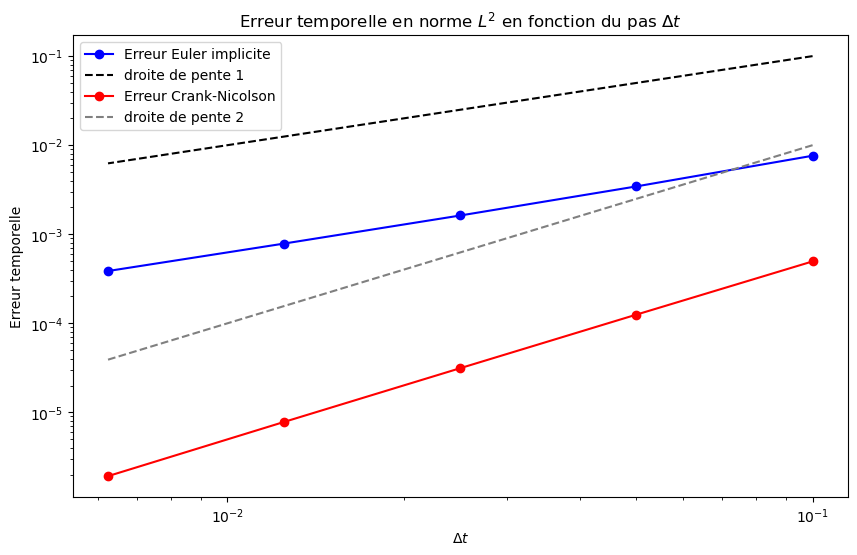
\includegraphics[width=\linewidth]{images/Crank-Nicolson/erreur_EI_CN.png}
    \caption{Comparaison Euler implicite et Crank-Nicolson}
    \label{fig:comparaison}
\end{figure}
\\\\
Ce graphique confirme nos résultats théoriques, le schéma d'Euler implicite est bien d'ordre $1$ en temps, celui de Crank-Nicolson est d'ordre $2$ en temps, il est donc plus précis que le schéma d'Euler implicite.

\newpage

% ===== Approximation par la méthode de DG ===== %
% =================================================================================
\section{Approximation par la méthode de Galerkin-Discontinu}
% =================================================================================
La méthode de Galerkin-Discontinu fait un lien entre les méthodes de volumes finis et d'éléments finis. En effet, on commence par écrire la formulation variationnelle et ensuite comme en élément fini on approche la solution théorique par une solution discrète à l'aide d'une combinaison linéaire de fonctions de base. \\
Même si les fonctions tests et les fonctions de base sont dans le même espace aucune continuité n'est imposé aux interfaces entre les éléments du maillage.
Nous prendrons une base polynomiale obtenu par un développement de Taylor. Il existe différent choix possible mais celui-ci permet une approche plus simple en ignorant la géométrie des mailles comme nous le verrons plus tard. \\
Nous allons commencer par étudier le cas $P_0$ où notre base est uniquement composée de la fonction constante égale à $1$, on retrouvera alors le schéma d'Euler implicite étudié précédemment. Puis, on pourra passer agrandir notre base en passant en $P_1$. Toute cette section s'inspire fortement des sources \cite{DiPietro2012}, \cite{FrancoisVilar2010} et \cite{Gerald2014}.
\\
On commence par partir du problème de Rayleigh-Stokes $1$D homogène
\begin{equation}
    \begin{cases}
        \partial_tu(t,x) - \nu\partial_{xx} u(t,x) - \alpha\partial_{txx} u(t,x) = 0 & (t,x) \in \mathbb R_+ \times \bbR  \\
        u(0,x) = u_0(x) & x \in \bbR
    \end{cases}
\end{equation}
On cherche alors a effectuer une formulation faible du problème en multipliant par une fonction test $v$ suffisamment régulière. En se plaçant sur une maille $K_i$ on peut alors écrire
\begin{equation*}
   \int_{K_i} \partial_t uv - \nu \int_{K_i}\partial_{xx}uv \ - \alpha \int_{K_i} \partial_{txx}uv = 0
\end{equation*}
En utilisant une formule de Green on obtient le résultat suivant
\begin{equation*}
    \int_{K_i} \partial_t uv + \nu \int_{K_i}\partial_{x}u\partial_{x}v \ + \alpha \int_{K_i} \partial_{tx}u\partial_{x}v
    =  \nu \int_{\partial K_i}(\partial_{x}u \cdot n)v \ + \alpha \int_{\partial K_i} (\partial_{tx}u \cdot n)v
\end{equation*}
Ce qui donne dans le cas $1$D
\begin{equation}\label{EDP_RS_Formulation_Faible}
    \int_{K_i} \partial_t uv + \nu \int_{K_i}\partial_{x}u\partial_{x}v \ + \alpha \int_{K_i} \partial_{tx}u\partial_{x}v
    =  \nu \Big[\partial_{x}u v \Big]^{x_i +h/2}_{x_i - h/2} \ + \alpha \Big[\partial_{tx}u v \Big]^{x_i +h/2}_{x_i - h/2} 
\end{equation}
Cette équation change grandement selon le choix de la base, par exemple pour une méthode Galerkin discontinu d'ordre 2, on obtient en faisait un développement de Taylor 
\begin{equation*}
    u(X) = u(X_i) + (X - X_i)\partial_X u(X_i) + \mathcal{O}\!\left((X - X_i)^2\right)
\end{equation*}
avec $X_i$ désignant le centroïde d'une cellule de longueur $h$.

Calculons la valeur moyenne $\bar{u}_i$ de notre inconnue sur une maille $K_i$
\begin{equation*}
\bar{u}_i = \frac{1}{h} \int_{K_i} u(X)\,dX = u(X_i) + \mathcal{O}\!\left(h^2\right)
\end{equation*}
Par conséquent
\begin{equation*}
u(X) = \bar{u}_i + h\,\partial_X u(X_i)\,\frac{X - X_i}{h} + \mathcal{O}\!\left(h^2\right)
\end{equation*}
On choisit alors la base $\{e_0, e_1\} = \left\{1, \dfrac{X - X_i}{h}\right\}$.
Le problème consiste donc à trouver $u_{h_{|K_i}} := u_h^i$, l'approximation de $u$ sur $K_i$, comme fonction de $\mathcal{P}^1(K_i)$ dans la base $\{e_j^i\}_{j=0,1}$ sous la forme 
\begin{equation}\label{base_formulation_varia_GD}
    u_h^i = \sum_{j=0}^{K} u_j^i(t)\, e_j^i(X) = u_0^i(t) + u_1^i(t)\,\frac{X - X_i}{h}
\end{equation}
Toute cette partie est bien écrite dans \cite[p.~29]{FrancoisVilar2010}.

\subsection{Etudes selon la taille de la base}
\subsubsection{Le cas \texorpdfstring{$P_0$}{P0}}
Dans le cas où l'on se contente de considérer la base  $\{e_0\} = \{ 1 \}$, on peut simplifier \eqref{EDP_RS_Formulation_Faible} qui prend en compte des $\partial v$ qui vaut $0$.
L'équation devient:
\begin{equation*}
    \int_{K_i} \partial_t u =  \nu \Big[\partial_{x}u \Big]^{x_i +h/2}_{x_i - h/2} \ + \alpha \Big[\partial_{tx}u \Big]^{x_i +h/2}_{x_i - h/2} 
\end{equation*}
En reprenant la formulation \eqref{base_formulation_varia_GD} cela se réécrit plus simplement:
\begin{equation}\label{EDP_RS_Formulation_Faible_P0}
    h\ \partial_t u_0^i = \nu \Big(\partial_{x}u_h^i\big|_{x_i + h/2} - \partial_{x}u_h^i\big|_{x_i - h/2} \Big) \ + \alpha \Big(\partial_{tx}u_h^i\big|_{x_i + h/2}- \partial_{tx}u_h^i\big|_{x_i - h/2}\Big) 
\end{equation}
\\
En reprenant la formulation \eqref{EDP_RS_Formulation_Faible_P0} il nous faut alors correctement définir le flux numérique. La trace $\partial_{x}u_h^i\big|_{x_i + h/2}$ n'est pas unique et est défini de chaque côté de l'interface. En $P0$ elle est même nulle puisque $u_h^i = u_0^i$ qui est constant sur les mailles. Donc on va ajouter un terme de pénalisation et utiliser le saut au niveau de chaque maille (voir \cite{DiPietro2012} page 125). Soit $\eta = 1$, on obtient alors:
\begin{equation*}
    \partial_x u_h\big|_{x_i + h/2} = \eta \frac{u_0^{i+1} - u_0^i}{h}, \qquad
    \partial_x u_h\big|_{x_i - h/2} = \eta \frac{u_0^i - u_0^{i-1}}{h}
\end{equation*}
En injectant dans l'équation on alors:
\begin{equation*}
    h\,\partial_t u_0^i = \nu\left(\frac{u_0^{i+1} - u_0^i}{h} - \frac{u_0^i - u_0^{i-1}}{h}\right)
    + \alpha\left(\frac{\partial_t u_0^{i+1} - \partial_t u_0^i}{h} - \frac{\partial_t u_0^i - \partial_t u_0^{i-1}}{h}\right)
\end{equation*}
ce qui se simplifie en :
\begin{equation*}
    h\,\partial_t u_0^i = \frac{\nu}{h}\left(u_0^{i+1} - 2u_0^i + u_0^{i-1}\right)
    + \frac{\alpha}{h}\left(\partial_t u_0^{i+1} - 2\partial_t u_0^i + \partial_t u_0^{i-1}\right)
\end{equation*}

En divisant par h on reconnaît exactement le schéma en différences finies :
\begin{equation*}
    \partial_t u_i - \nu\Delta_h u_i - \alpha\Delta_h\!\left(\partial_t u_i\right) = 0
\end{equation*}
où $\Delta_h u_i = \dfrac{u_{i+1} - 2u_i + u_{i-1}}{h^2}$. \\
On résout alors le problème de façon similaire au chapitre \ref{Chapitre_3}. Numériquement, les résultats sont similaires :
\begin{figure}[H]
    \centering
    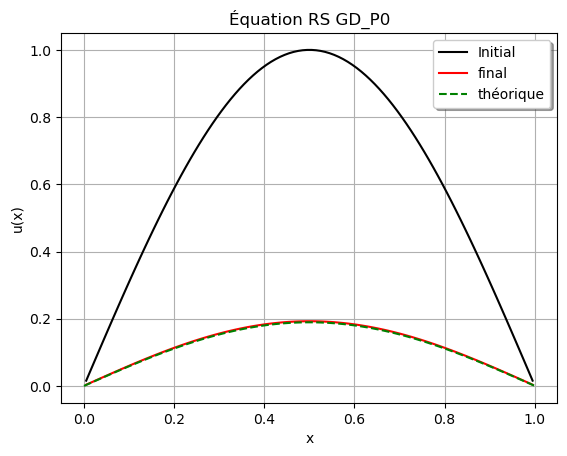
\includegraphics[width=0.5\linewidth]{images/DG/P0.png}
    \caption{Résolution par GDP0}
    \label{GDP0}
\end{figure}

\subsubsection{Le cas \texorpdfstring{$P_1$}{P1}}
On prend désormais la base $\{\phi_0, \phi_1\} = \left\{1,\  \dfrac{X - X_i}{h}\right\}$. La solution approché $u_h$ s'écrit (dans cette base et sur la i-ème maille): $ u_h = u^0_i \phi_0 + u^1_i \phi_1$. \\
En remplaçant cette nouvelle expression dans \ref{EDP_RS_Formulation_Faible} on obtient (Pour $j = 0 , 1$):
\begin{eqnarray*}\label{EDP_RS_Formulation_Faible_P1}
  &\partial_t u_i^0 \int_{K_i}  \phi_0 \phi_j + \partial_t u_i^1 \int_{K_i}  \phi_1 \phi_j& \\
   &+\nu \ u_i^0  \int_{K_i}\partial_{x}\phi_0 \partial_{x}\phi_j  + \nu \ u_i^1 \int_{K_i}\partial_{x}\phi_1 \partial_{x}\phi_j& \\
   &+ \alpha \partial_{t}u_i^0 \int_{K_i} \partial_{x}\phi_0\partial_{x}\phi_j + \alpha \partial_{t}u_i^1 \int_{K_i} \partial_{x}\phi_1\partial_{x}\phi_j &\\
    &=& \\ 
    &\nu \Big[\partial_{x}\big(u_i^0\phi_0 +u_i^1\phi_1 \big) \phi_j  \Big]^{x_i +h/2}_{x_i - h/2} \ + \alpha \Big[\partial_{tx}\big(u_i^0\phi_0 +u_i^1\phi_1 \big) \phi_j \Big]^{x_i +h/2}_{x_i - h/2} 
\end{eqnarray*}
On calcule les matrices de l'expression précédente.
\begin{eqnarray*}
    &&\int_{K_i}  \phi_0 \phi_0 = \int_{K_i}  1 = h \\
    &&\int_{K_i}  \phi_0 \phi_1 = \int_{K_i} \frac{x -x_i}{h} = 0 \\
    &&\int_{K_i}  \phi_1 \phi_1 = \int_{K_i} \bigg(\frac{x -x_i}{h}\bigg)^2 = \frac{h}{12} \\
    &&\int_{K_i}  \partial\phi_0 \partial\phi_0 = \int_{K_i}  \partial\phi_0 \partial\phi_1= 0 \\
    &&\int_{K_i}  \partial\phi_1 \partial\phi_1 = \frac{1}{h^2} 
\end{eqnarray*}

Il nous faut alors encore traiter les valeurs aux interfaces correctement. Cette fois la trace du gradient de $u_h$ ne s'annule pas et vaut $\frac{u_i^1}{h}$ sur la maille $K_i$ et  $\frac{u_{i+1}^1}{h}$ sur la maille $K_{i+1}$
On définit alors le flux moyen à chaque interface (qui va remplacer la trace du gradient) comme: $\{\!\!\{ u_i^1 \}\!\!\}_{F_i} = \frac{u_{i}^{1} + u_{i+1}^{1}}{2h}$ où $F = K_i \cap K_{i+1}$ \\
Maintenant que tout est bien défini on peut écrire le système suivant:

\begin{eqnarray*}
    &&\begin{bmatrix}
        h & 0 \\
        0 & \frac{h}{12} 
    \end{bmatrix}
    \begin{bmatrix}
    \partial_t u_i^0 \\
    \partial_t u_i^1    
    \end{bmatrix}
    +
        \begin{bmatrix}
        0 & 0 \\
        0 & \frac{\nu + \alpha \partial_t}{h} 
    \end{bmatrix}
    \begin{bmatrix}
    u_i^0 \\
    u_i^1    
    \end{bmatrix}
    = (\nu + \alpha\partial_t)
    \begin{bmatrix}
    \{\!\!\{ u_i^1 \}\!\!\}_{F_i} - \{\!\!\{ u_i^1 \}\!\!\}_{F_{i-1}}\\
    \{\!\!\{ u_i^1 \}\!\!\}_{F_i} \times\frac{1}{2} - \{\!\!\{ u_i^1 \}\!\!\}_{F_{i-1}} \times (- \frac{1}{2})
    \end{bmatrix} \\
    \\
    &&\begin{bmatrix}
        h & 0 \\
        0 & \frac{h}{12} 
    \end{bmatrix}
    \begin{bmatrix}
    \partial_t u_i^0 \\
    \partial_t u_i^1    
    \end{bmatrix}
    +
        \begin{bmatrix}
        0 & 0 \\
        0 & \frac{\nu + \alpha \partial_t}{h} 
    \end{bmatrix}
    \begin{bmatrix}
    u_i^0 \\
    u_i^1    
    \end{bmatrix}
    = (\nu + \alpha\partial_t)
    \begin{bmatrix}
    \frac{u_{i+1}^1 - u_{i-1}^1 }{2h}\\
    \frac{u_{i+1}^1 - u_{i-1}^1 }{4h}
    \end{bmatrix}
\end{eqnarray*}
Qui se réécrit plus simplement :
\begin{eqnarray*}
    M \partial_t U + C U = B
\end{eqnarray*}

Pour approcher la dérivée en temps on utilise Euler Explicite. On pourra alors calculer la solution $U$ au temps $n+1$ en fonction de $U$ au temps $n$ sur une maille $K_i$.\\
Cette approche est certainement trop brutale car elle ne permet pas d'adapter facilement la montée en ordre de la méthode ce qui est sensé être un des avantages de Galerkin Discontinu. Il faut certainement repartir de la formulation variationnelle et réussir à exprimer ça de façon plus générale...

On trouve un exemple qui correspond à une version simplifié de notre équation dans "\cite{Gerald2014}" (page 193 à 196)
"Un premier choix dit « naïf », pour le flux numérique de la dérivée spatiale est un flux numérique centré". Notre façon de faire et donc simpliste et peut présenter des problèmes plus tard mais reste une première approche acceptable.
% Je trouve ça un peu partout:Le terme de bord issu de l'IPP sur $K_i$ s'écrit, en utilisant le flux numérique centré
%$\widehat{\sigma}_{i\pm 1/2} := \{\{ \partial_x u_h \}\}_{ i \pm 1/2}$:



















\newpage

% --- CONCLUSION --- %
% ==================================================================================
% Introduction 
% ==================================================================================

\thispagestyle{empty}
\vspace*{1cm}

\begin{center}
    \Large\textbf{Conclusion}
\end{center}

Ce travail encadré de recherche nous a permis de réaliser un projet de groupe sur le long terme, le projet étant d'étudier l'équation de Rayleigh-Stokes. Nous avons choisis ce sujet car il nous permettait d'aborder tout les aspects de notre formation. 
\\
Dans un premier temps, la partie modélisation, en lisant l'article sur le premier problème de Stokes \cite{Christov2010} nous avons pu utiliser notre cours de mécanique et ainsi mieux comprendre le modèle et sa dérivation. 
\\
Ensuite, la partie analyse mathématique avec d'abord une analyse de Fourier dans laquelle nous avons grandement utilisé le cours d'Analyse des EDP2. Cette analyse nous a permis de démontrer l'existence et l'unicité d'une solution dans différents espaces. Cette équation est liée à l'équation de la chaleur puisqu'on retrouve celle-ci en prenant $\alpha=0$, l'analyse de Fourier nous a aussi permis de comparer le comportement de la solution de l'équation de Rayleigh-Stokes avec la solution de l'équation de la chaleur et ainsi mettre en évidence une propriété de filtre passe-bas due, justement, au terme $\alpha$.
\\
Puis, nous avons suivi l'approche menée dans l'article de Showalter et Ting \cite{Showalter_Ting} pour résoudre le problème par une formulation variationnelle. Cette méthode nous a conduits à utiliser les notions d'Analyse numérique $3$ pour obtenir une formulation faible du problème. Le résultat important de cette partie est bien entendu le théorème \ref{thm_lax}, il nous a permis de reformuler le problème pour pouvoir utiliser la théorie des semi-groupes, que nous avions légèrement abordées durant le cours d'Analyse des EDP2. Pour terminer, la modélisation mécanique nous a amené à une équation vectorielle dont le cas n'était pas étudié dans l'article \cite{Showalter_Ting}, nous avons alors tenté de reproduire le raisonnement utilisé pour l'équation scalaire pour l'équation vectorielle. Ce raisonnement n'a pas été très difficile à adapter, cependant le cadre théorique autour de l'équation vectorielle était bien plus compliqué à aborder et l'adaptation de celui-ci n'a pas toujours été fructueuse. Il nous faudra donc revenir sur le cadre théorique et les résultats associés à celui-ci.
\\
Enfin, le dernier aspect de notre formation : l'analyse numérique. Nous avons commencé par définir un schéma différence finie d'Euler implicite. L'étude de ce schéma montre qu'il est consistant d'ordre un en temps et deux en espace et stable, donc il est convergent. Mais l'étude de la stabilité nous a permis de mettre en évidence, comme pour l'analyse de Fourier, la propriété de filtre passe-bas de la solution due une nouvelle fois au terme $\alpha$. Selon l'ordre de grandeur de $\alpha$ devant $\nu$ on a l'amortissement immédiat des hautes fréquences. Puis nous avons comparé ces résultats avec ceux pour l'équation de la chaleur sur un profil sinusoïdal, ce qui nous a conduit une nouvelle fois à remarquer l'importante influence du paramètre $\alpha$ sur le comportement de la solution.
\\
Nous avons ensuite implémenté quelques cas tests ayant une interprétation physique intéressante que nous pouvions liée à notre cours de Mécanique ainsi qu'avec l'article \cite{Christov2010}. Pour finir, nous avons implémenté un schéma différence finie de Crank-Nicolson dans le but de monter en ordre en temps. On a alors obtenu une schéma consistant d'ordre deux en temps et en espace, toujours stable et donc convergent.
\\
Et, nous avons terminé la partie analyse numérique par une tentative d'approche par la méthode de Galerkin discontinue. Cette approche nous a permis de voir un lien entre les méthodes volumes finis et éléments finis et de commencer à lire la documentation liée à cette méthode(\cite{DiPietro2012} et \cite{Gerald2014}). Nous avons pu implémenter le cas $P_0$ qui est similaire aux différences finies cependant le cas $P_1$ semble présenter encore quelques problèmes notamment au niveau de la gestion du flux moyen. Cela nous pousse à continuer d'étudier le choix des flux les plus adaptés pour les équations pseudo-paraboliques.

\newpage


% --- ANNEXES --- %
% =================================================================================
% ANNEXES
% =================================================================================
\renewcommand{\appendixtocname}{Annexes}
\renewcommand{\appendixpagename}{Annexes}

\begin{appendices}
% ---------------------------------------------------------------------------------
\section{Démonstration du théorème \ref{thm_lax}}\label{AnnexeA}
% ---------------------------------------------------------------------------------
On rappelle l'énoncé du théorème.
\begin{theoreme}
Soient $(H, \langle \cdot, \cdot \rangle)$ et $(H_0, \langle \cdot, \cdot \rangle_0)$ deux espaces de Hilbert tels que $H$ est un sous-espace dense de $H_0$
et 
\begin{equation}\label{norm_equiv_H_H0}
    \exists k >0,\ \forall x \in H, \ \norm{x} \geq k \norm{x}_0
\end{equation}
Soit $B$ une forme bilinéaire continue et coercive sur $H$. Alors il existe deux opérateurs linéaires $E$ et $E^*$, dont les domaines de définitions $D$ et $D^*$ sont denses dans $H$, tels que
\begin{enumerate}
    \item On a
    \begin{eqnarray*}
        \forall x \in D,\ \forall y \in H, \ B(x,y) &=& \ps{Ex}{y}_0 \\
        \forall y \in D^*,\ \forall x \in H, \ B(x,y) &=& \ps{x}{E^* y}_0
    \end{eqnarray*}
    \item L'image de $E$ est $H_0$, de même pour $E^*$.
    \item $E$ et $E^*$ admettent des inverses $S$ et $S^*$ qui sont continus de $H_0$ dans $H$.
    \begin{eqnarray*}
        \exists k_1>0,\ \forall z \in H_0, \ \norm{Sz} &\leq& k_1 \norm{z}_0 \\
        \exists k_1^*>0,\ \forall z \in H_0, \ \norm{S^*z} &\leq& k_1^* \norm{z}_0
    \end{eqnarray*}
    Et donc, $S$ et $S^*$ sont continus de $H_0$ dans $H_0$
    \begin{eqnarray*}
        \exists k_2>0,\ \forall z \in H_0, \ \norm{Sz}_0 &\leq& k_2 \norm{z}_0 \\
        \exists k_2^*>0,\ \forall z \in H_0, \ \norm{S^*z}_0 &\leq& k_2^* \norm{z}_0
    \end{eqnarray*}
\end{enumerate}
\end{theoreme}

\begin{proof}
    On se contentera de montrer le théorème pour $E$ car pour $E^*$ le raisonnement sera identique mais portera sur le deuxième argument de la forme bilinéaire $B$. Ceci s'explique par le fait que $B$ n'est pas symétrique.
    \\
    Soit $z \in H_0$. On peut définir une forme linéaire $\ell$ sur $H$ par 
    \begin{equation*}
        \forall x \in H, \ \ell(x) = \langle z, x \rangle_0
    \end{equation*}
    On a $\ell \in H'$, en effet par Cauchy-Schwarz on a 
    \begin{equation*}
        \forall x \in H, \ |\ell(x)| = |\langle z, x \rangle_0| \overset{\eqref{norm_equiv_H_H0}}{\leq} \frac{1}{k}\|z\|_0 \|x\|
    \end{equation*}
    On considère le problème : trouver $y \in H$ tel que 
    \begin{equation}\label{proof_pbm_var}
        \forall x \in H, \ B(y,x) = \ell(x)
    \end{equation}
    On a montré que $\ell$ est continue sur $H$ et par hypothèse, $B$ est continue et coercive sur $H$ donc par le théorème de Lax-Milgram il existe un unique $y \in H$ tel que \eqref{proof_pbm_var} soit satisfaite. Cette solution $y$ dépend de $z$ et ce $z$ étant quelconque dans $H_0$, ce raisonnement est valable pour tout $z \in H_0$. On définit ainsi une application 
    \begin{equation*}
        S : H_0 \rightarrow H, \ z \mapsto S(z) = y
    \end{equation*}
    Autrement dit, cette application $S$ associe à chaque $z \in H_0$ la solution $y \in H$ au problème \eqref{proof_pbm_var} où $\ell = \langle z, \cdot \rangle_0$.
    A présent, montrons les propriétés de $S$.
    \begin{itemize}
        \item Montrons que $S$ est linéaire.
        \\
        Soient $z,z' \in H_0$ et $\lambda \in \bbR$. Par définition, il existe $y, y' \in H$ tels que 
        \begin{eqnarray}\label{proof_eg1}
            \forall x \in H, \ B(y,x) &=& \langle z,x \rangle_0 \nonumber \\
            \forall x \in H, \ B(y',x) &=& \langle z',x \rangle_0
        \end{eqnarray}
        On peut multiplier la première égalité par $\lambda$ et utiliser les propriétés de linéarité pour obtenir 
        \begin{equation}\label{proof_eg2}
            \forall x \in H, \ B(\lambda y, x) = \langle \lambda z, x\rangle_0
        \end{equation}
        On somme \eqref{proof_eg1} et \eqref{proof_eg2}, ce qui donne en utilisant à nouveau la linéarité
        \begin{eqnarray*}
            \forall x \in H, \ B(\lambda y + y',x) = \langle \lambda z+z', x \rangle_0
        \end{eqnarray*}
        Ainsi,
        \begin{eqnarray*}
            S(\lambda z+z') = \lambda y+y' = \lambda S(z) + S(z')
        \end{eqnarray*}
        d'où la linéarité de $S$.
        \item Montrons que $D:=S(H_0)$ est dense dans $H$. On notera plus simplement $\overline{D}:=\overline{D}^H$, car nous ne regarderons par $\overline{D}^{H_0}$.
        \\
        Tout d'abord, $D$ est un sous-espace vectoriel de $H$ car $H_0$ est un espace vectoriel et $S$ est une application linéaire. Donc $\overline{D}$ est aussi un sous-espace vectoriel de $H$. Supposons par l'absurde que $\overline{D} \subsetneq H$. Alors $\overline{D}$ est un sous-espace vectoriel fermé de $H$ donc $\{0\} \subsetneq \overline{D}^{\perp}$ (on utilisera dans la suite le fait que l'orthogonal \og ne voit pas \fg{} l'adhérence, \textit{i.e.} $\overline{D}^{\perp} = D^{\perp}$). Soit $z \in D^{\perp}$ tel que $z\neq 0$. On considère le problème \eqref{proof_pbm_var}, en utilisant une nouvelle le théorème de Lax-Milgram, on obtient l'existence d'un unique $y \in H$ vérifiant \eqref{proof_pbm_var}. On a $y=Sz \in D \subset H$ et la coercivité de $B$ donne (on note $\alpha >0$ la constante de coercivité)
        \begin{equation*}
            \alpha \|y\|^2 \leq B(y,y) = \langle z,y \rangle_0 = 0
        \end{equation*}
        donc $y=0$. Ainsi, on a
        \begin{equation*}
            \forall x \in H, \ \langle z, x \rangle_0 = 0
        \end{equation*}
        En particulier, pour $x=z$ on obtient $\|z\|_0^2=0$ donc $z=0$ ce qui est absurde. Donc $\overline{D} = H$.
        \item Montrons que $S : H_0 \rightarrow D$ admet un inverse.
        \\
        Par définition, $S : H_0 \rightarrow D$ est surjective. Montrons qu'elle est injective. Soient $v,w \in H_0$ tels que $Sv = Sw$. On a alors par définition de $S$
        \begin{eqnarray*}
            \forall x \in H, \ B(Sv, x) = \langle v,x \rangle_0 \ \ \ &\text{ et }& \ \ \ B(Sw,x)=\langle w,x\rangle_0
        \end{eqnarray*}
        en utilisant l'hypothèse, on obtient 
        \begin{eqnarray*}
            \forall x \in H, \ \langle v,x \rangle_0 = \langle w, x \rangle_0 &\Longrightarrow& \langle v-w, x \rangle_0=0
        \end{eqnarray*}
        donc $v-w \in H^\perp = \overline{H}^\perp = H_0^\perp=\{0\}$ donc $v=w$. Ainsi, $S$ admet un inverse que l'on note $E$ et on a bien 
        \begin{equation*}
            \forall x \in D, \ \forall y \in H, B(x,y) = \langle S^{-1}x,y\rangle_0 = \langle Ex, y \rangle_0
        \end{equation*}
        \item Montrons que $S$ est continue de $H_0$ dans $H$ et de $H_0$ dans lui-même.
        \\
        Par coercivité de $B$, on a pour tout $z \in H_0$
        \begin{equation*}
            \alpha \|Sz\|^2 \leq B(Sz,Sz) = \langle z, Sz \rangle_0 \overset{\text{C-S}}{\leq} \|z\|_0\|Sz\|_0 \overset{\eqref{norm_equiv_H_H0}}{\leq} \frac{1}{k}\|z\|_0\|Sz\|
        \end{equation*}
        d'où la continuité de $H_0$ dans $H$
        \begin{equation*}
            \|Sz\|_0 \leq \frac{1}{\alpha k} \|z\|_0
        \end{equation*}
        et en utilisant à nouveau \eqref{norm_equiv_H_H0} on obtient le continuité de $H_0$ dans lui-même
        \begin{equation*}
            \forall z \in H_0, \ \|Sz\|_0 \leq \frac{1}{k}\|Sz\| \leq \frac{1}{\alpha k^2}\|z\|_0
        \end{equation*}
    \end{itemize}
\end{proof}

\newpage

% ---------------------------------------------------------------------------------
\section{Démonstration du théorème \ref{thm_densite}}\label{AnnexeB}
% ---------------------------------------------------------------------------------
Commançons par rappeller les notations. On considère l'espace de 
Hilbert 
\begin{equation*}
    V = \{ \bfm{v} \in \big(\Hone\big)^d \ \ | \ \ \Div(\bfm{v})=0\}
\end{equation*}
et l'espace 
\begin{equation*}
    \calD_{\sigma}(\Omega) = \{\bfm{\varphi} \in \big(\calD(\Omega)\big)^d \ \ | \ \ \Div(\bfm{\varphi})=0\}
\end{equation*}
Montrons dans un premier temps que $V$ est un espace de Hilbert. 
On sait que $\Hone$ est un Hilbert, donc $\big(\Hone\big)^d$ est 
un Hilbert comme produit d'espace de Hilbert. On a clairement
\begin{equation*}
    V \subset \big(\Hone\big)^d
\end{equation*}
donc, pour montrer que $V$ est un Hilbert, il suffit de montrer que 
$V$ est fermé dans $\big(\Hone\big)^d$. On considère l'application 
$\Div : \big(L^2(\Omega)\big)^d \rightarrow H^{-1}(\Omega)$. Cette application est continue,
en effet, soit $\bfm{u} \in \big(L^2(\Omega)\big)^d$ et soit $\varphi \in \calD(\Omega)$.
\begin{eqnarray*}
    |\langle \Div(\bfm{u}),\varphi \rangle| &=& |\langle \sum_{i=1}^d \partial_i u_i , \varphi \rangle| \\
    &=& \bigg|\sum_{i=1}^d \langle \partial_i u_i, \varphi \rangle\bigg| \\
    &=& \bigg|-\sum_{i=1}^d \langle u_i, \partial_i\varphi \rangle\bigg| \\
    &=& \bigg|\sum_{i=1}^d \int_{\Omega} u_i \partial_i\varphi \bigg| \\
    &=& \bigg|\int_{\Omega} \bfm{u}\cdot\nabla \varphi\bigg| \\
    &\overset{\text{C-S}}{\leq}& \|\bfm{u}\|_{L^2}\|\nabla \varphi\|_{L^2} \\
    &\leq& \|\bfm{u}\|_{L^2}\|\varphi \|_{H^1}
\end{eqnarray*} 
Donc en particulier, $\Div : \big(\Hone\big)^d \rightarrow H^{-1}(\Omega)$ est continue et donc 
$V= \Div^{-1}\big(\{0\}\big)$ est fermé dans $\big(\Hone\big)^d$ comme 
image réciproque d'un fermé par une application continue.
\\\\
Passons à présent à la démonstration du théorème \ref{thm_densite}, on rappelle l'énoncé
\begin{theoreme}
    Si $\Omega \subset \bbR^d$ est un ouvert borné à la frontière
    suiffisamment régulière alors $\calD_{\sigma}(\Omega)$
    est dense dans $V$.
\end{theoreme}

\begin{proof}
    Comme $\calD(\Omega)$ est dense dans $\Hone$, $\big(\calD(\Omega)\big)^d$
    est dense dans $\big(\Hone\big)^d$. Soit $\bfm{v} \in V$. Alors il 
    existe $(\bfm{\varphi}_n)_{n \in \bbN} \subset \big(\calD(\Omega)\big)^d$
    telle que $\bfm{\varphi}_n\underset{n \to +\infty}{\overset{\Hone^d}{\longrightarrow}} \bfm{v}$, 
    cependant rien ne dit que 
    \begin{equation*}
        \forall n \in \bbN, \ \Div(\bfm{\varphi}_n) = 0
    \end{equation*}
    On pose 
    \begin{equation*}
        \forall n \in \bbN, \ f_n := \Div(\bfm{\varphi}_n) \in \calD(\Omega)
    \end{equation*}
    Comme $\Div(\bfm{v})=0$, on a 
    \begin{equation*}
        f_n = \Div(\bfm{\varphi}_n) - \Div(\bfm{v}) = \Div(\bfm{\varphi}_n-\bfm{v})
    \end{equation*}
    et par continuité de $\Div$
    \begin{equation*}
        \|f_n\|_{L^2} \leq \|\bfm{\varphi}_n -\bfm{v}\|_{H^1} \underset{n \to +\infty}{\longrightarrow} 0
    \end{equation*}
    De plus, par le théorème de la divergence on a
    \begin{equation*}
        \int_{\Omega}f_n = \int_{\Omega} \Div(\bfm{\varphi}_n) = \int_{\partial \Omega} \bfm{\varphi}_n \cdot n = 0
    \end{equation*}
    donc $(f_n)_{n \in \bbN} \subset L^2_0(\Omega)$ l'ensemble des fonctions de $L^2(\Omega)$ de moyenne nulle.
    Par le théorème de De Rahm, il existe un opérateur continu
    $T : L^2_0(\Omega) \rightarrow \big(\Hone\big)^d$ tel que 
    \begin{equation*}
        \forall q \in L_0^2(\Omega), \ \Div(Tq) = q
    \end{equation*}
    On considère à présent la suite définie par 
    \begin{equation*}
        \forall n \in \bbN, \ \bfm{\psi}_n := Tf_n \in \big(\Hone\big)^d
    \end{equation*}
    On a par continuité de $T$, 
    \begin{equation*}
        \|\bfm{\psi}_n\|_{H^1} \leq C \|f_n\|_{L^2} \underset{n \to +\infty}{\longrightarrow} 0
    \end{equation*}
    On pose maintenant 
    \begin{equation*}
        \forall n \in \bbN, \ \bfm{v}_n := \bfm{\varphi}_n - \bfm{\psi}_n 
    \end{equation*}
    Ansi, 
    \begin{eqnarray*}
        \Div(\bfm{v}_n) = \Div(\bfm{\varphi}_n) - \Div(\bfm{\psi}_n)
        = \Div(\bfm{\varphi}_n) - \Div(Tf_n) = \Div(\bfm{\varphi}_n) - f_n = 0
    \end{eqnarray*}
    Finalement, on obtient 
    \begin{equation*}
        \|\bfm{v}-\bfm{v}_n\|_{H^1} \leq \|\bfm{v}-\bfm{\varphi}_n\|_{H^1}+\|\bfm{\psi}_n\|_{H^1} \underset{n \to +\infty}{\longrightarrow} 0
    \end{equation*}
\end{proof}

\begin{remark}
    La suite $(\bfm{v}_n)_{n \in \bbN}$ n'est pas dans $\calD_{\sigma}(\Omega)$
    donc le théorème n'est pas démontré.
\end{remark}

\newpage

% ---------------------------------------------------------------------------------
%\section{}
% ---------------------------------------------------------------------------------

\end{appendices}
\newpage


% --- BIBLIOGRAPHIES --- %
% =================================================================================
% BIBLIOGRAPHIE
% =================================================================================
\addcontentsline{toc}{section}{Références}

%\subsection*{Articles de référence}
%\begin{itemize}
    %\item Jean-François Coulombel. \textit{Stability of finite difference schemes for hyperbolic initial boundary value problems}. DEA. France. 2011, pp.99. ⟨cel-00616497⟩
%\end{itemize}

\nocite{*}
\printbibliography

\paragraph{Manuels et Cours}
\begin{itemize}
    \item Bellieud, M. (2026). \textit{Cours de mécanique des milieux continus}. Université de Montpellier.
    \item Marche, F. (2026). \textit{Analyse des EDP 2}. Université de Montpellier.
    \item Gallo, C. (2026). \textit{Analyse des EDP 1}. Université de Montpellier.
    \item Vilar, F. (2026). \textit{Analyse numérique 1 \& 2}. Université de Montpellier.
\end{itemize}



\end{document}